\chapter{Diseño Dinámico}

El presente capítulo detalla el comportamiento en tiempo de ejecución del sistema SICORRE para los casos de uso principales. A continuación, se presentan los diagramas de secuencia que modelan la interacción entre los diferentes componentes del sistema (Usuario, Interfaz, Backend y Base de Datos) junto con sus flujos de excepción y flujos alternativos.

% ============================================================
\section{Diseño Dinámico del CU: Iniciar sesión (CU-01)}
% ============================================================

\subsection*{Descripción del Flujo}
El usuario (Administrador o Especialista) accede a la interfaz de inicio de sesión de SICORRE. Proporciona su correo electrónico y contraseña. La interfaz realiza una validación local (campos no vacíos y formato de correo electrónico). Al presionar el botón de inicio, se envía una petición HTTP POST con las credenciales cifradas al controlador de autenticación en el Backend. El Backend recibe los datos y consulta la base de datos para recuperar la información del usuario por su correo. La base de datos responde con el registro del usuario (incluyendo password hash, rol y estado activo). El Backend valida que el hash coincida y que la cuenta no esté revocada. Tras una verificación exitosa, el Backend genera un token de acceso JWT y lo envía a la interfaz. Finalmente, la interfaz almacena el token de sesión en el almacenamiento local del navegador y redirige al usuario a su panel de control correspondiente a su rol asignado.

\begin{figure}[H]
	\centering
	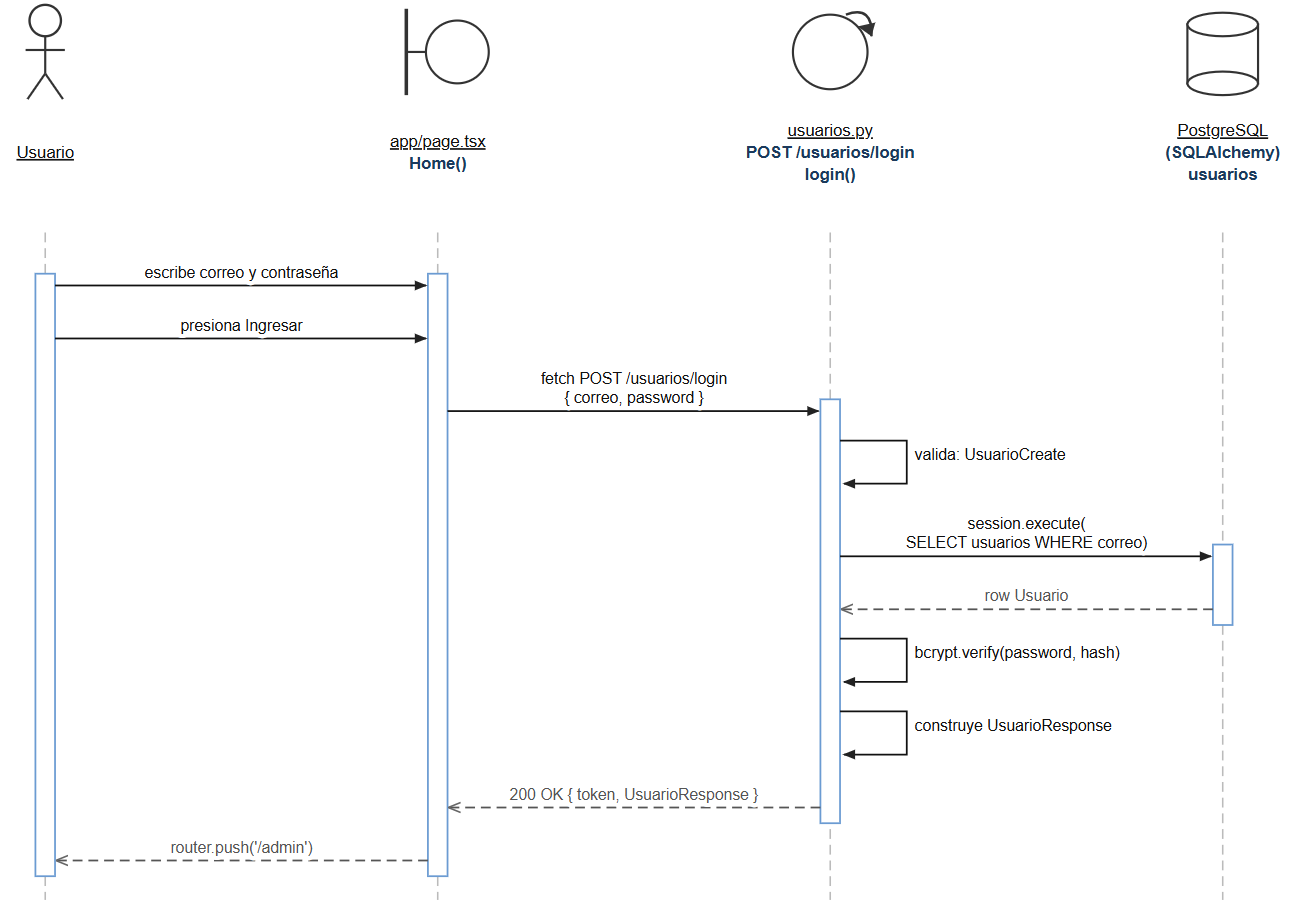
\includegraphics[width=0.8\textwidth]{img/CU01.png}
	\caption{Diagrama de secuencia --- CU-01 Iniciar sesión.}
	\label{fig:secuencia-cu01}
\end{figure}

\subsection*{Flujo Alternativo / Excepciones}
\begin{itemize}
	\item \textbf{E1: Credenciales incorrectas} - El correo electrónico o la contraseña ingresados no coinciden con ningún registro activo en la base de datos. El sistema muestra el mensaje "Correo o contraseña inválidos" y limpia el campo de contraseña.
	\item \textbf{E2: Usuario inactivo o revocado} - El usuario existe pero su estado en la base de datos es inactivo. El sistema niega el acceso, muestra el mensaje de cuenta revocada y cancela el inicio de sesión.
	\item \textbf{E3: Campos obligatorios incompletos} - La interfaz detecta que uno o ambos campos del formulario están vacíos. Se detiene la petición y se muestra un mensaje de advertencia visual en los campos correspondientes.
\end{itemize}

\bigskip
\noindent\rule{\linewidth}{0.5pt}
\bigskip

% ============================================================
\section{Diseño Dinámico del CU: Cerrar sesión (CU-02)}
% ============================================================

\subsection*{Descripción del Flujo}
El usuario activo hace clic en el botón de cerrar sesión ubicado en la barra de navegación del sistema. La interfaz de usuario envía una solicitud de invalidación al controlador de sesión en el Backend. El Backend procesa la solicitud, invalida el token JWT activo en la lista de sesiones y responde con un mensaje de éxito. Al recibir la respuesta, la interfaz de usuario elimina por completo el token de acceso y cualquier dato de sesión del almacenamiento local del navegador (localStorage y sessionStorage). Finalmente, redirige al usuario de manera inmediata a la pantalla de inicio de sesión, bloqueando la navegación hacia atrás mediante el historial del navegador.

\begin{figure}[H]
	\centering
	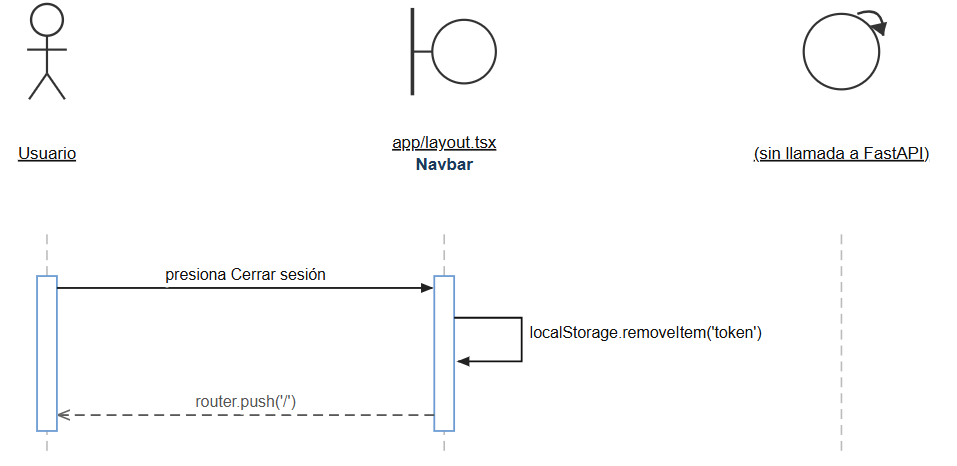
\includegraphics[width=0.8\textwidth]{img/CU02.png}
	\caption{Diagrama de secuencia --- CU-02 Cerrar sesión.}
	\label{fig:secuencia-cu02}
\end{figure}

\subsection*{Flujo Alternativo / Excepciones}
\begin{itemize}
	\item \textbf{E1: Error de comunicación con el servidor} - Si ocurre una falla de red al notificar al backend, la interfaz de usuario de todas formas borra el token local por razones de seguridad y fuerza la redirección a la pantalla de inicio de sesión.
\end{itemize}

\bigskip
\noindent\rule{\linewidth}{0.5pt}
\bigskip

% ============================================================
\section{Diseño Dinámico del CU: Recuperar contraseña (CU-03)}
% ============================================================

\subsection*{Descripción del Flujo}
El usuario presiona el enlace "¿Olvidó su contraseña?" en la pantalla de inicio de sesión. La interfaz presenta un formulario solicitando el correo electrónico de la cuenta. El usuario ingresa su correo electrónico y presiona "Enviar enlace". La interfaz valida el formato y envía la solicitud al Backend. El Backend consulta la base de datos para verificar que el correo corresponda a un usuario activo. Al confirmarse, el Backend genera un token de recuperación único con tiempo de expiración limitado y lo registra en la base de datos. Posteriormente, el Backend compone y envía un correo electrónico al usuario con un enlace seguro que contiene el token. El sistema notifica al usuario en pantalla que las instrucciones han sido enviadas a su correo electrónico.

\begin{figure}[H]
	\centering
	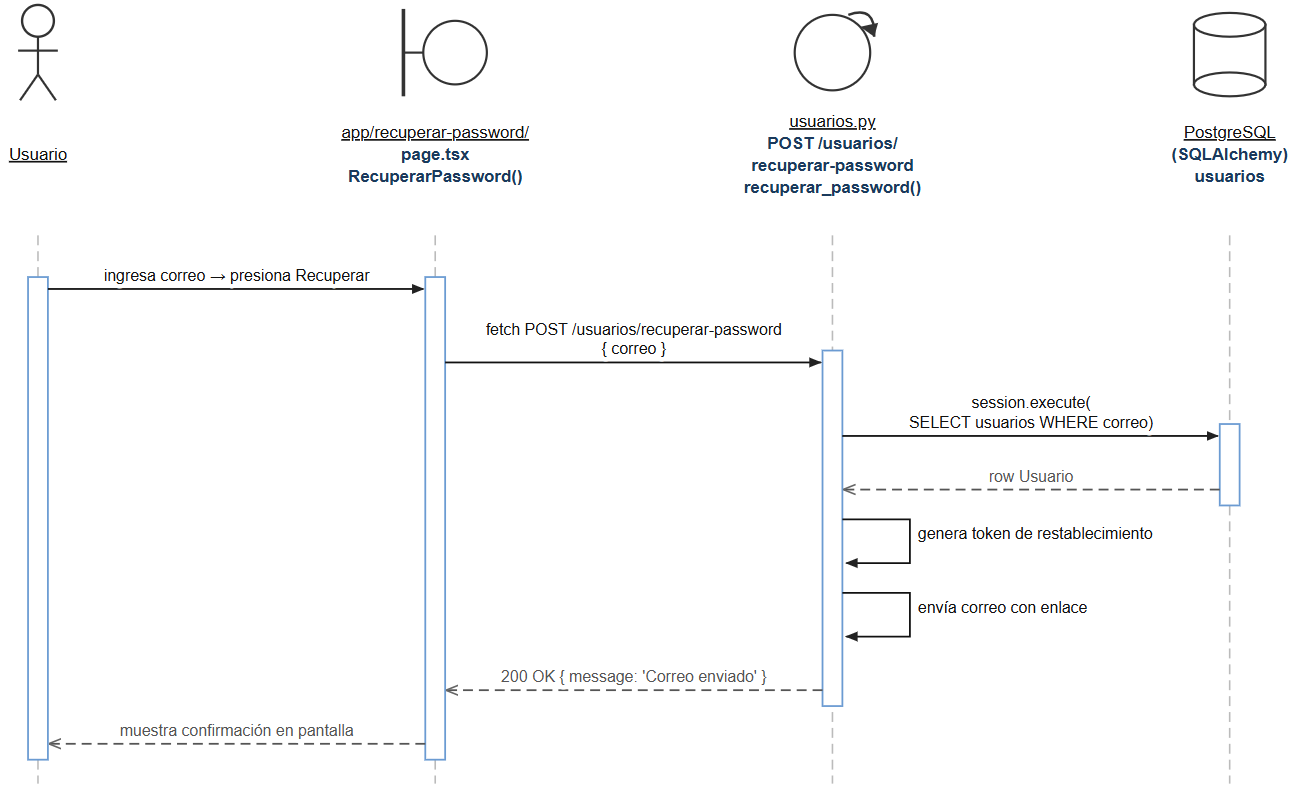
\includegraphics[width=0.8\textwidth]{img/CU03.png}
	\caption{Diagrama de secuencia --- CU-03 Recuperar contraseña.}
	\label{fig:secuencia-cu03}
\end{figure}

\subsection*{Flujo Alternativo / Excepciones}
\begin{itemize}
	\item \textbf{E1: Correo electrónico no registrado} - El correo electrónico proporcionado no coincide con ningún usuario en el sistema. El sistema muestra un mensaje indicando que no se pudo procesar la solicitud para ese correo por seguridad.
	\item \textbf{E2: Cuenta de usuario inactiva} - Si el correo corresponde a un usuario cuyo acceso ha sido revocado, el sistema deniega la generación del token y muestra un aviso de error de seguridad.
\end{itemize}

\bigskip
\noindent\rule{\linewidth}{0.5pt}
\bigskip

% ============================================================
\section{Diseño Dinámico del CU: Registrar usuario (CU-04)}
% ============================================================

\subsection*{Descripción del Flujo}
El Administrador accede al formulario de registro de personal. Captura los datos personales (nombre, CURP, fecha de nacimiento, sexo), domicilio (apoyado por el catálogo de SEPOMEX), rol del usuario (Administrador o Especialista) e información de contacto (teléfono y correo electrónico). La interfaz valida que todos los campos obligatorios estén provistos. Al presionar "Guardar", la interfaz envía los datos al Backend. El Backend verifica en la base de datos que el correo electrónico y la CURP ingresados no estén duplicados. Si son únicos, genera una contraseña temporal, la encripta y guarda el nuevo usuario en la base de datos. Finalmente, el Backend envía un correo automático al nuevo usuario con sus credenciales provisionales y responde con éxito a la interfaz, que redirige al listado de usuarios.

\begin{figure}[H]
	\centering
	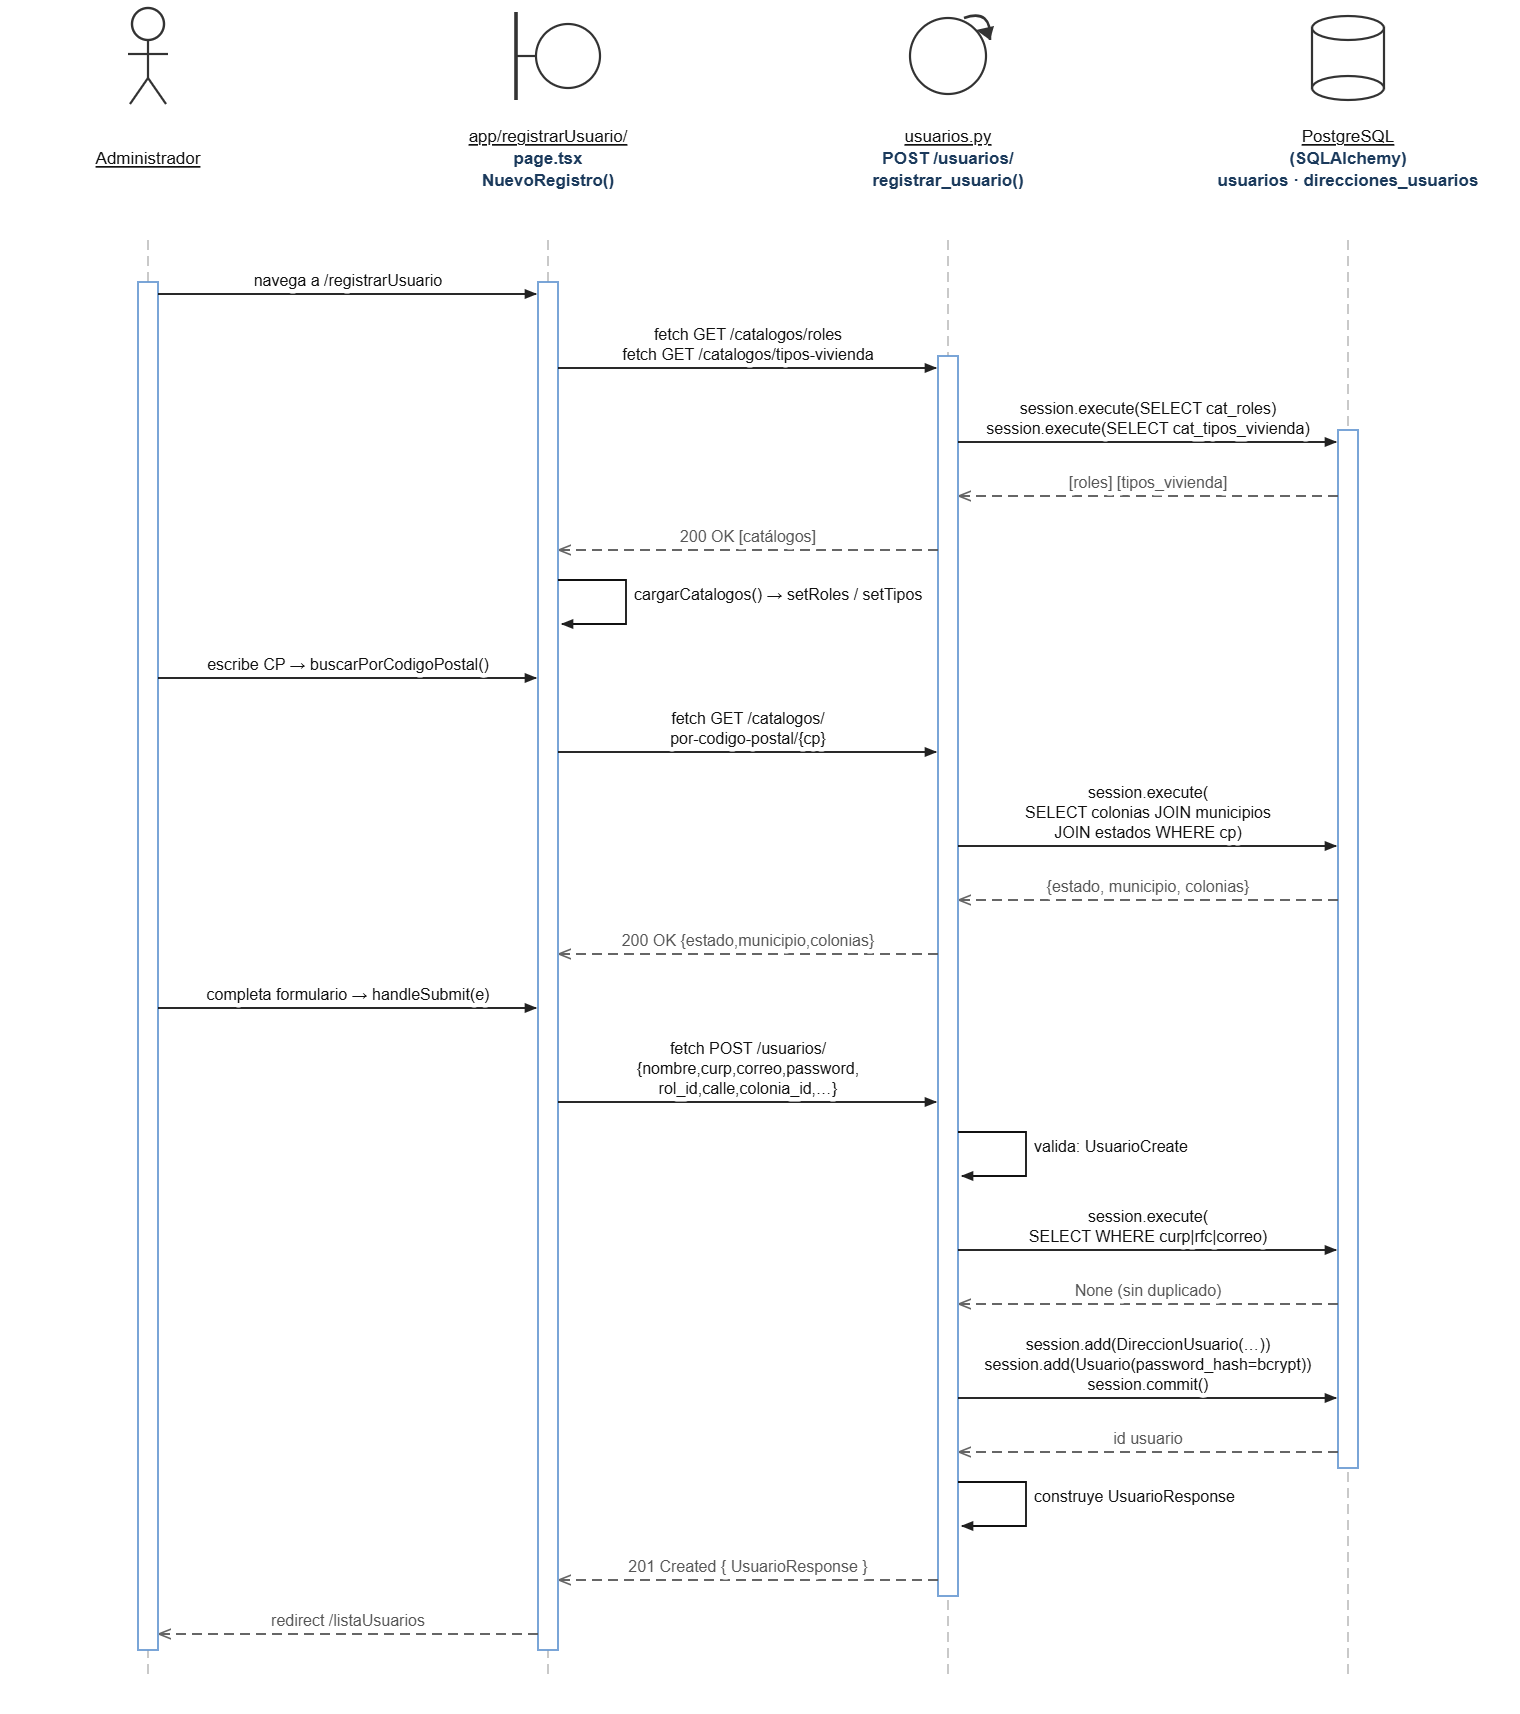
\includegraphics[width=0.8\textwidth]{img/CU-04.png}
	\caption{Diagrama de secuencia --- CU-04 Registrar usuario.}
	\label{fig:secuencia-cu04}
\end{figure}

\subsection*{Flujo Alternativo / Excepciones}
\begin{itemize}
	\item \textbf{E1: Correo electrónico ya registrado} - El correo proporcionado ya está asociado a otro usuario. El sistema muestra el mensaje "El correo ingresado ya existe" y solicita cambiarlo.
	\item \textbf{E2: CURP ya registrada} - La CURP ingresada ya se encuentra en el sistema. Se muestra el mensaje "La CURP ingresada ya existe" y detiene el registro.
	\item \textbf{E3: Campos obligatorios incompletos} - Si se omiten campos obligatorios en el formulario, el sistema despliega el mensaje "Campos obligatorios incompletos" y resalta los campos vacíos.
\end{itemize}

\bigskip
\noindent\rule{\linewidth}{0.5pt}
\bigskip

% ============================================================
\section{Diseño Dinámico del CU: Consultar usuario (CU-05)}
% ============================================================

\subsection*{Descripción del Flujo}
El Administrador accede a la sección de control de personal de la plataforma. La interfaz realiza una solicitud de consulta general al Backend. El Backend ejecuta una consulta select en la base de datos para extraer los registros de los usuarios registrados, incluyendo su nombre, rol, CURP, correo electrónico y estado de cuenta (Activo/Inactivo). La base de datos devuelve el listado de usuarios. El Backend procesa la información y la envía a la interfaz, que la renderiza en una tabla interactiva que permite al Administrador buscar, filtrar y seleccionar registros específicos para ver su ficha detallada.

\begin{figure}[H]
	\centering
	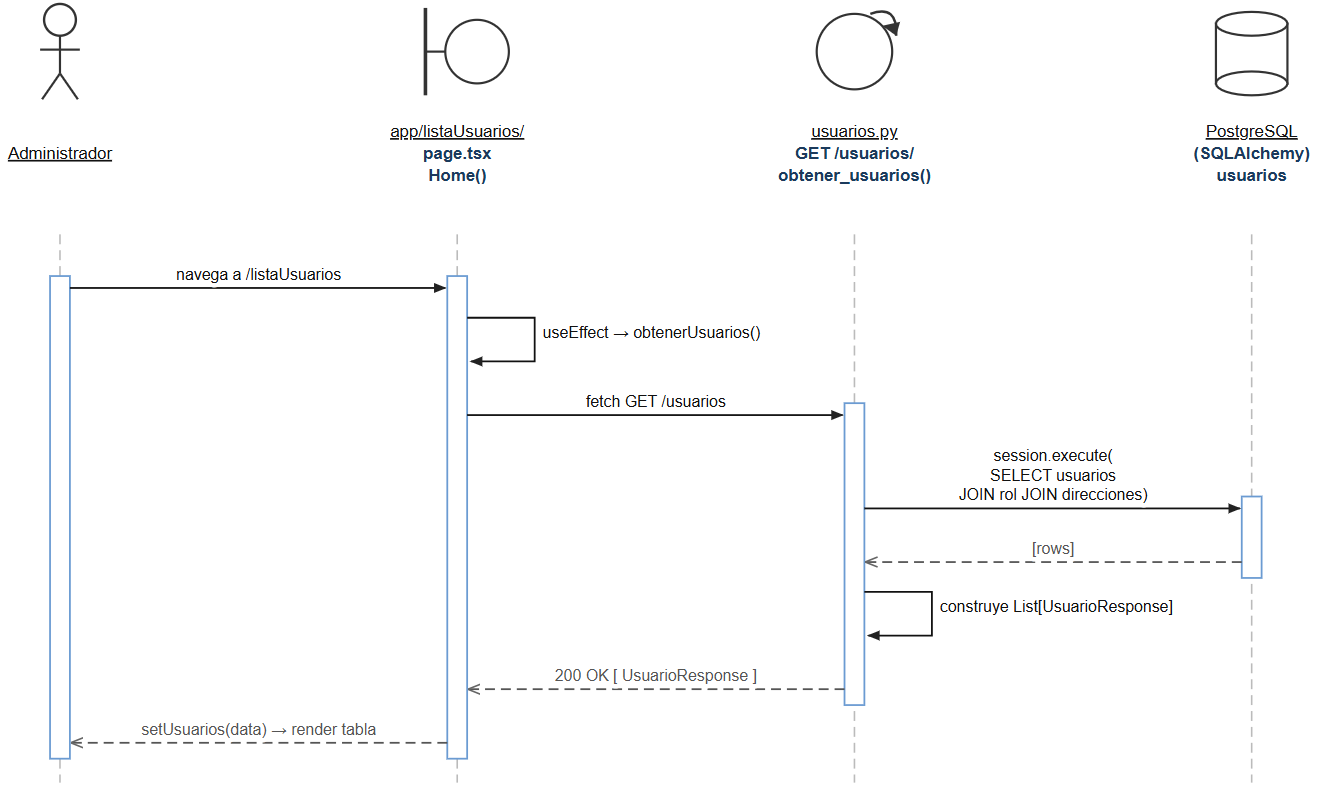
\includegraphics[width=0.8\textwidth]{img/CU05.png}
	\caption{Diagrama de secuencia --- CU-05 Consultar usuario.}
	\label{fig:secuencia-cu05}
\end{figure}

\subsection*{Flujo Alternativo / Excepciones}
\begin{itemize}
	\item \textbf{E1: No existen usuarios registrados} - Si la base de datos está vacía, el sistema muestra una tabla sin registros junto con el mensaje "Sin usuarios registrados".
\end{itemize}

\bigskip
\noindent\rule{\linewidth}{0.5pt}
\bigskip

% ============================================================
\section{Diseño Dinámico del CU: Modificar usuario (CU-06)}
% ============================================================

\subsection*{Descripción del Flujo}
El Administrador selecciona un usuario del listado y hace clic en "Modificar". La interfaz solicita los datos detallados del usuario al Backend y los carga precargados en el formulario de edición. El Administrador modifica los datos necesarios (datos personales, dirección, rol o estado) y presiona "Guardar cambios". La interfaz envía los datos modificados al Backend. El Backend valida que los datos no colisionen con los de otros usuarios (verificando que la CURP o correo electrónico no pertenezcan a otro ID de usuario diferente). Si la validación es correcta, el Backend actualiza el registro del usuario en la base de datos y responde con éxito a la interfaz, la cual muestra un mensaje de confirmación exitosa.

\begin{figure}[H]
	\centering
	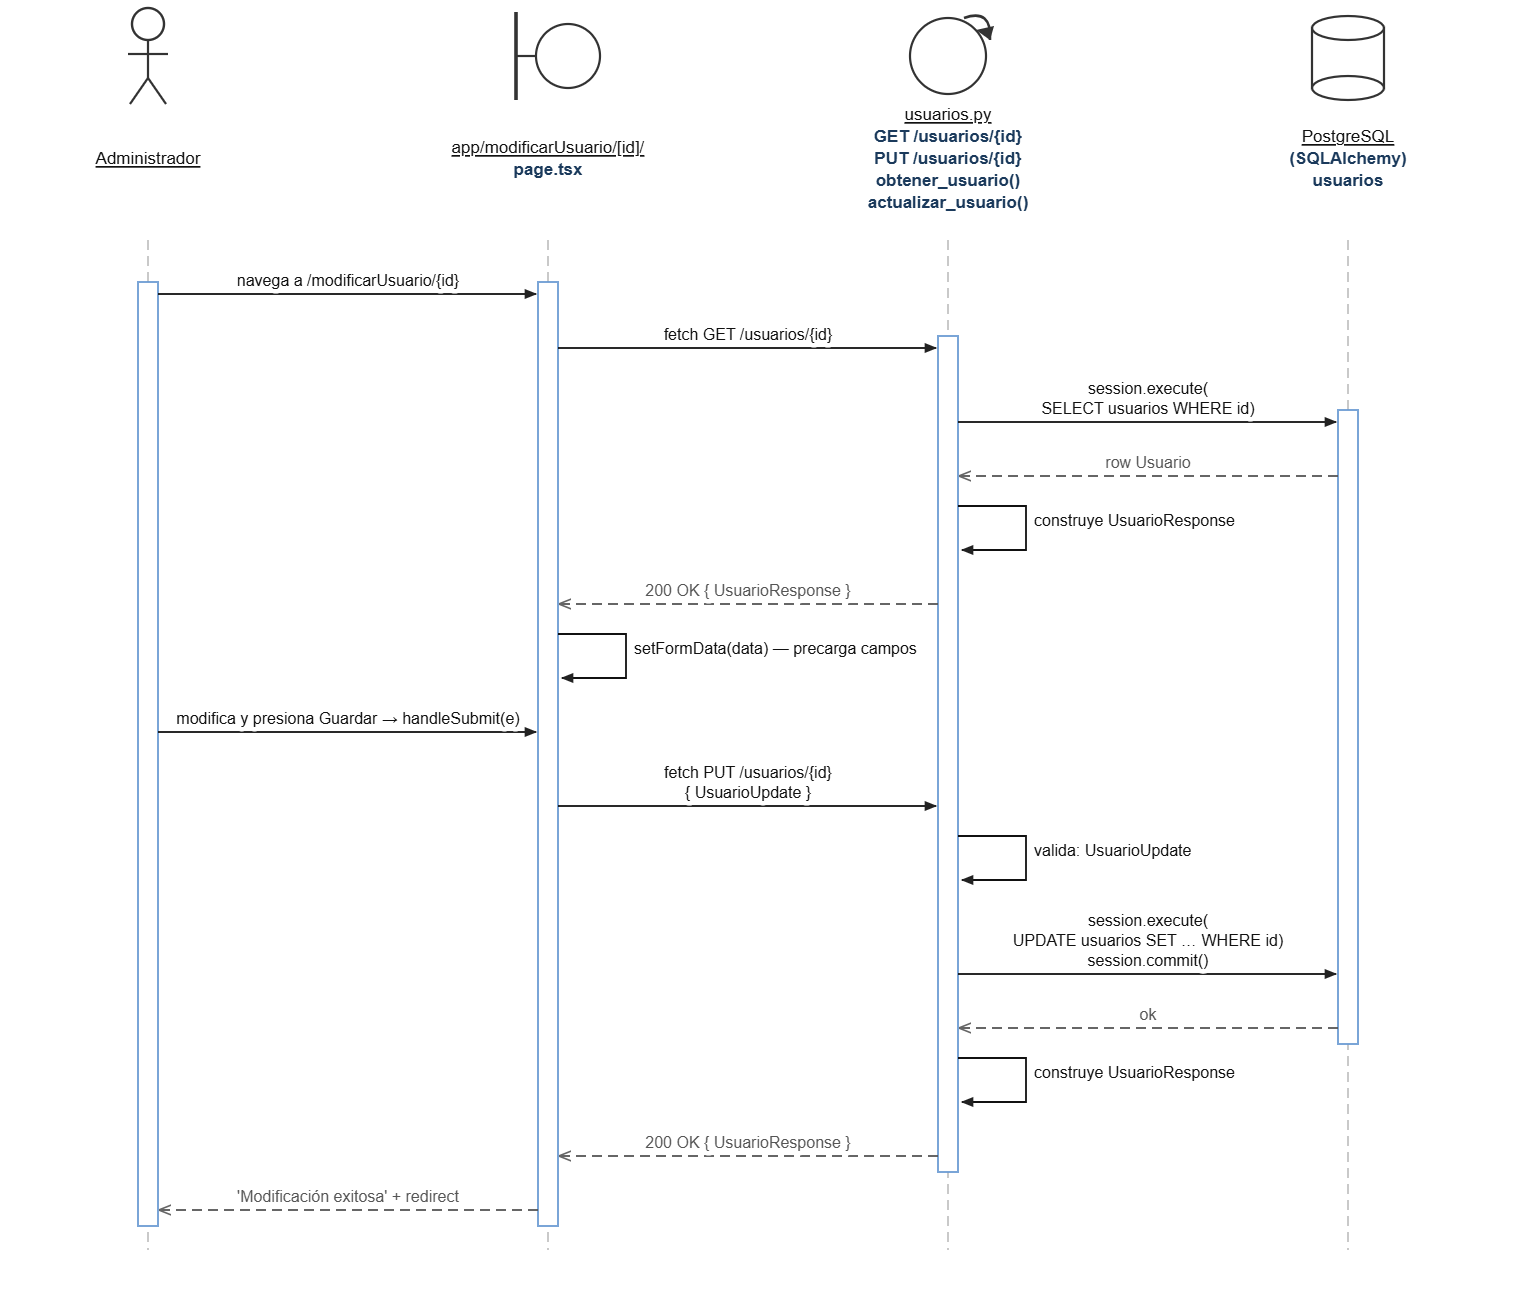
\includegraphics[width=0.8\textwidth]{img/CU-06.png}
	\caption{Diagrama de secuencia --- CU-06 Modificar usuario.}
	\label{fig:secuencia-cu06}
\end{figure}

\subsection*{Flujo Alternativo / Excepciones}
\begin{itemize}
	\item \textbf{E1: Correo electrónico duplicado} - El correo modificado ya pertenece a otro usuario registrado. El sistema muestra un mensaje de error y no guarda los cambios.
	\item \textbf{E2: CURP duplicada} - La CURP modificada ya está registrada para otro usuario. Se notifica del error y se regresa al formulario.
	\item \textbf{E3: Campos requeridos vacíos} - Si se eliminan datos obligatorios del formulario, el sistema bloquea el guardado e indica cuáles campos deben llenarse.
\end{itemize}

\bigskip
\noindent\rule{\linewidth}{0.5pt}
\bigskip

% ============================================================
\section{Diseño Dinámico del CU: Revocar acceso a usuario (CU-07)}
% ============================================================

\subsection*{Descripción del Flujo}
El Administrador localiza un usuario activo en el listado de personal y hace clic en la opción "Revocar acceso". La interfaz muestra un modal de confirmación advirtiendo sobre la inhabilitación del acceso de dicho usuario. Al confirmar la acción, la interfaz envía una solicitud de desactivación al Backend. El Backend actualiza el estado del usuario a "Inactivo" en la base de datos, destruyendo adicionalmente cualquier sesión y token de acceso JWT asociado a dicho usuario en el caché de sesiones. El Backend responde con la confirmación de la revocación y la interfaz actualiza visualmente el estado del usuario en el listado.

\begin{figure}[H]
	\centering
	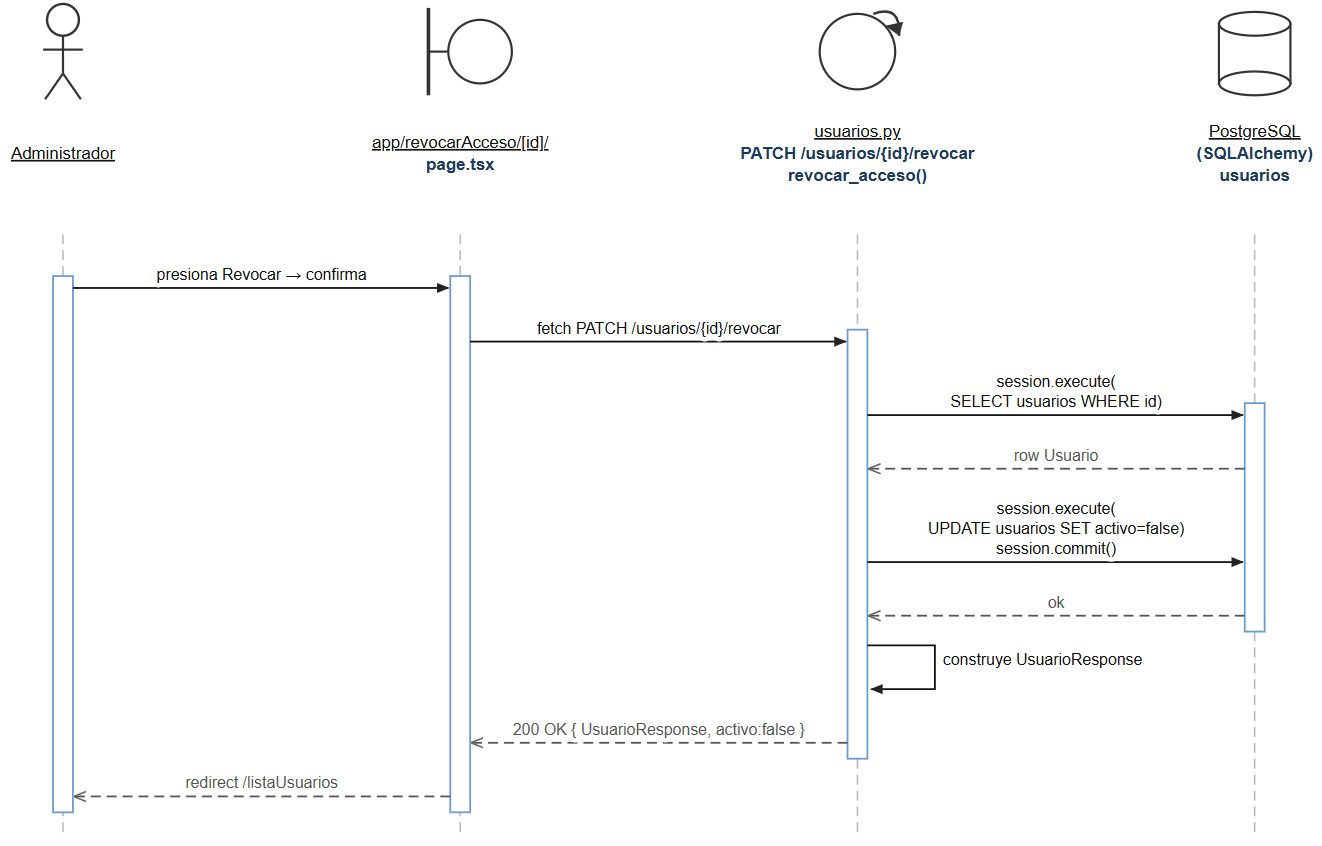
\includegraphics[width=0.8\textwidth]{img/CU07.png}
	\caption{Diagrama de secuencia --- CU-07 Revocar acceso a usuario.}
	\label{fig:secuencia-cu07}
\end{figure}

\subsection*{Flujo Alternativo / Excepciones}
\begin{itemize}
	\item \textbf{E1: Cancelación de la confirmación} - El Administrador cancela la acción en el modal. La interfaz cierra la ventana y mantiene el estado del usuario sin cambios.
	\item \textbf{E2: Intento de autorevocación} - El Administrador intenta revocar su propia cuenta de acceso activa. El sistema detecta que el ID coincide con el usuario autenticado, bloquea la acción y muestra un mensaje de error indicando que no puede autorevocarse.
\end{itemize}

\bigskip
\noindent\rule{\linewidth}{0.5pt}
\bigskip

% ============================================================
\section{Diseño Dinámico del CU: Eliminar usuario (CU-08)}
% ============================================================

\subsection*{Descripción del Flujo}
El Administrador selecciona a un usuario en el listado de personal y hace clic en "Eliminar". La interfaz despliega un cuadro de diálogo solicitando la confirmación de la eliminación definitiva. Al confirmar la acción, la interfaz envía la solicitud al Backend. El Backend realiza una verificación de integridad referencial en la base de datos para confirmar que el usuario no tiene dependencias activas (como expedientes a su cargo, pertenencia a equipos multidisciplinarios o participación en eventos programados). Si el usuario está libre de dependencias, el Backend ejecuta la eliminación del registro de la base de datos y devuelve éxito. La interfaz actualiza el listado de personal.

\begin{figure}[H]
	\centering
	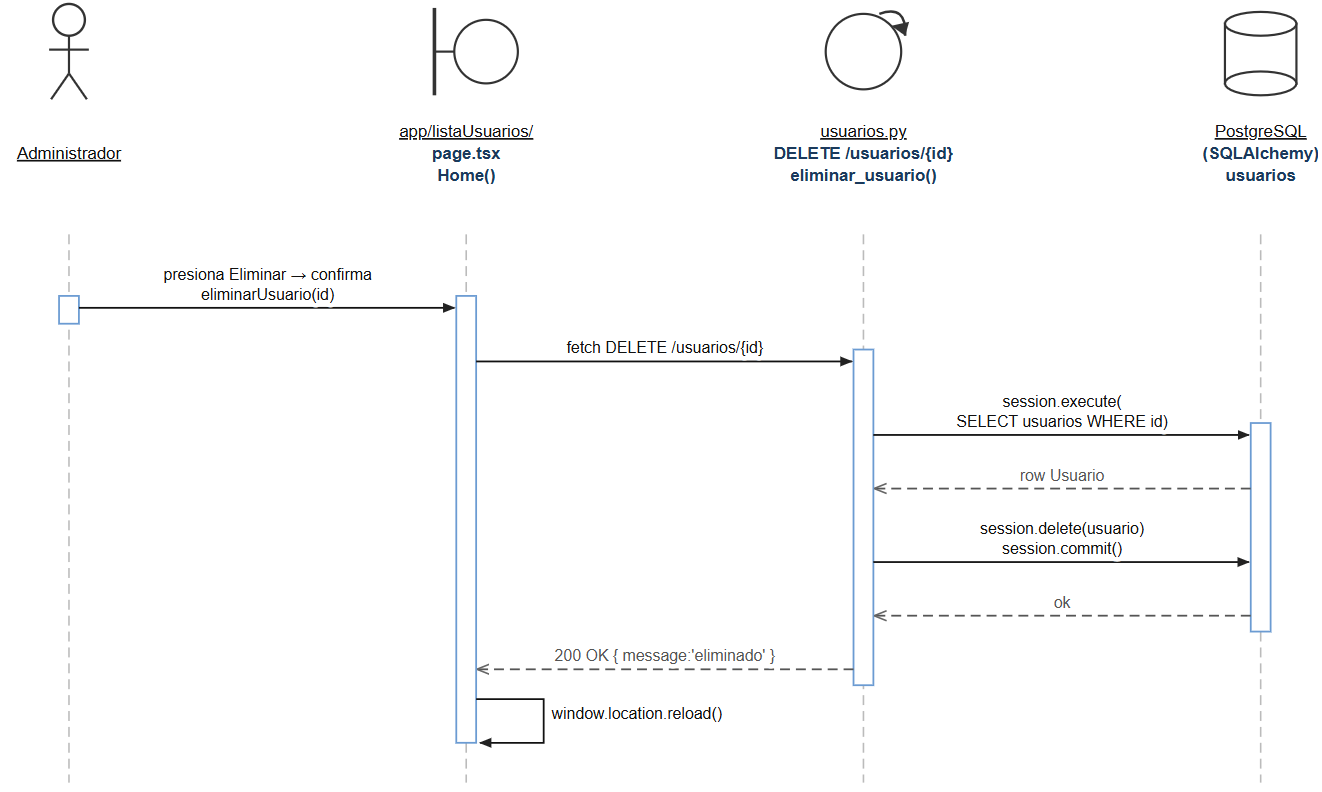
\includegraphics[width=0.8\textwidth]{img/CU08.png}
	\caption{Diagrama de secuencia --- CU-08 Eliminar usuario.}
	\label{fig:secuencia-cu08}
\end{figure}

\subsection*{Flujo Alternativo / Excepciones}
\begin{itemize}
	\item \textbf{E1: Usuario con dependencias activas} - El usuario tiene expedientes o asignaciones activas asociadas en el sistema. El Backend rechaza la solicitud de eliminación por integridad referencial y responde con un error. La interfaz muestra un mensaje sugiriendo revocar el acceso en su lugar.
	\item \textbf{E2: Cancelación de la eliminación} - El Administrador cancela la acción en el modal. La interfaz cierra el cuadro de diálogo sin realizar modificaciones.
\end{itemize}

\bigskip
\noindent\rule{\linewidth}{0.5pt}
\bigskip

% ============================================================
\section{Diseño Dinámico del CU: Registrar equipo multidisciplinario (CU-09)}
% ============================================================

\subsection*{Descripción del Flujo}
El Administrador accede al módulo de administración y selecciona "Crear Equipo Multidisciplinario". Introduce el nombre propuesto para el equipo. Al presionar "Guardar", la interfaz envía los datos al Backend. El Backend valida que el nombre del equipo no esté vacío y realiza una consulta en la base de datos para comprobar que no exista otro equipo con el mismo nombre. Si el nombre está libre, inserta el nuevo registro del equipo multidisciplinario en la base de datos con estado "Activo". El Backend retorna un mensaje de éxito y la interfaz redirige al Administrador a la consulta de equipos.

\begin{figure}[H]
	\centering
	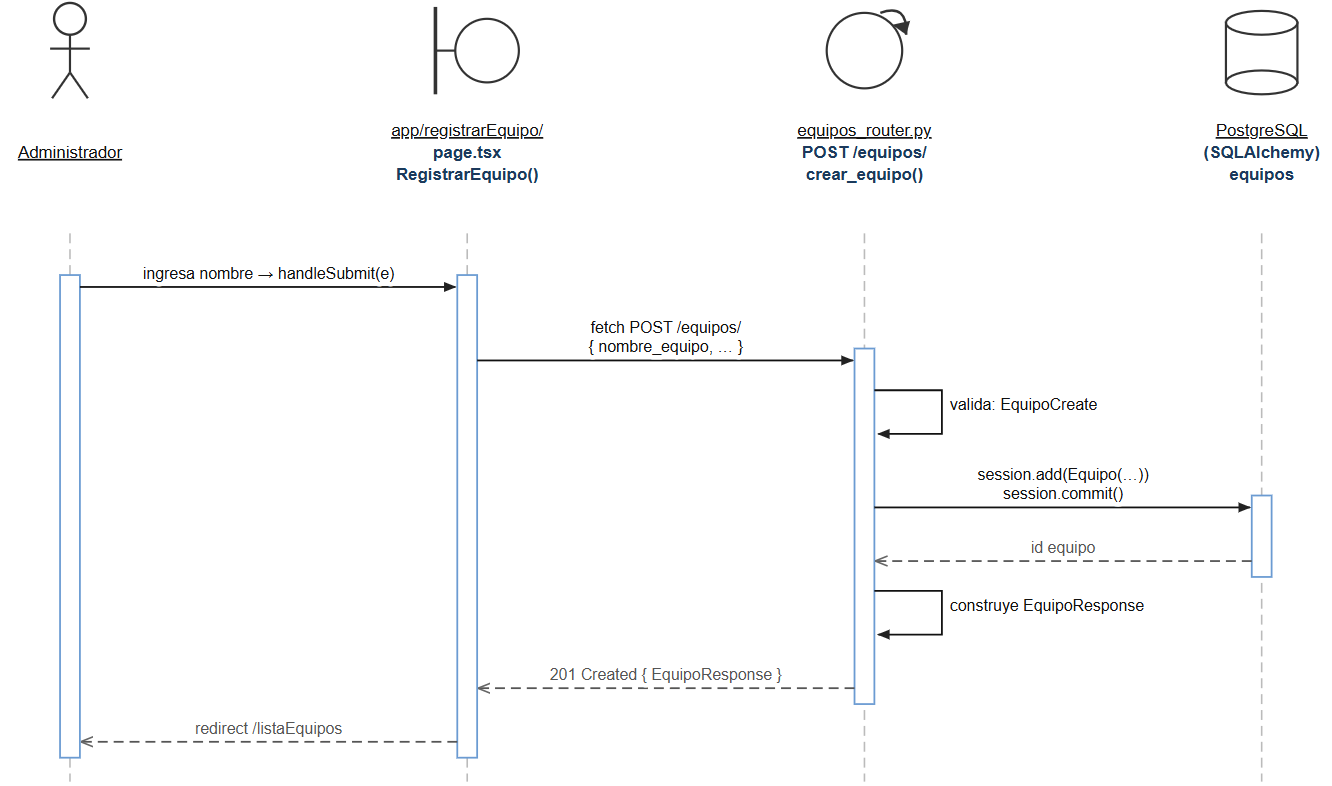
\includegraphics[width=0.8\textwidth]{img/CU09.png}
	\caption{Diagrama de secuencia --- CU-09 Registrar equipo multidisciplinario.}
	\label{fig:secuencia-cu09}
\end{figure}

\subsection*{Flujo Alternativo / Excepciones}
\begin{itemize}
	\item \textbf{E1: Nombre del equipo ya registrado} - Ya existe un equipo multidisciplinario con el nombre proporcionado en la base de datos. El sistema muestra el mensaje "El nombre de equipo ingresado ya existe" y detiene la creación.
	\item \textbf{E2: Campo de nombre vacío} - El Administrador intenta guardar sin especificar un nombre. La interfaz intercepta la acción, muestra una advertencia y evita el envío.
\end{itemize}

\bigskip
\noindent\rule{\linewidth}{0.5pt}
\bigskip

% ============================================================
\section{Diseño Dinámico del CU: Consultar equipo multidisciplinario (CU-10)}
% ============================================================

\subsection*{Descripción del Flujo}
El Especialista o Administrador ingresa al submódulo de Equipos Multidisciplinarios. La interfaz solicita la información de los equipos al Backend. El Backend ejecuta una consulta select en la base de datos uniendo las tablas de equipos, personal e integrantes asociados para recuperar la información completa (nombre del equipo, miembros que lo conforman por especialidad y total de expedientes de NNA que tienen asignados). La base de datos devuelve los registros correspondientes. El Backend estructura la información en un formato JSON y la envía a la interfaz, que la renderiza en una vista organizada por tarjetas o acordeones interactivos.

\begin{figure}[H]
	\centering
	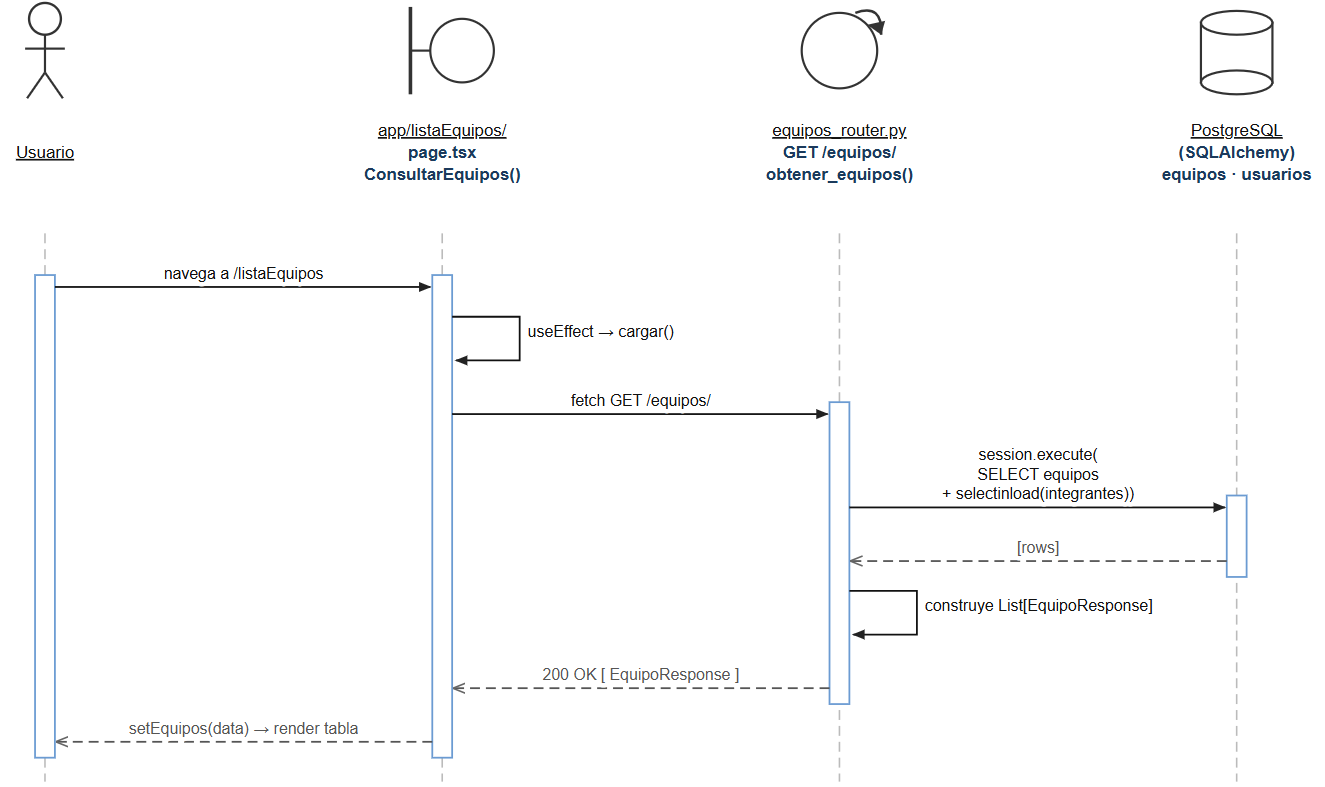
\includegraphics[width=0.8\textwidth]{img/CU10.png}
	\caption{Diagrama de secuencia --- CU-10 Consultar equipo multidisciplinario.}
	\label{fig:secuencia-cu10}
\end{figure}

\subsection*{Flujo Alternativo / Excepciones}
\begin{itemize}
	\item \textbf{E1: No existen equipos registrados} - La consulta a la base de datos retorna una lista vacía. La interfaz muestra un mensaje indicando que no hay equipos multidisciplinarios registrados actualmente en el sistema.
\end{itemize}

\bigskip
\noindent\rule{\linewidth}{0.5pt}
\bigskip

% ============================================================
\section{Diseño Dinámico del CU: Modificar equipo multidisciplinario (CU-11)}
% ============================================================

\subsection*{Descripción del Flujo}
El Administrador selecciona un equipo del listado y presiona "Editar". La interfaz solicita los datos detallados del equipo y la lista de personal disponible al Backend y los carga en pantalla. El Administrador edita el nombre del equipo, añade nuevos integrantes (Especialista en Psicología, Trabajo Social o Derecho) o remueve miembros existentes. Al guardar, la interfaz transmite los cambios al Backend. El Backend comprueba que el nombre del equipo no colisione con otro y que no se dupliquen especialidades clave de manera inapropiada. Posteriormente, actualiza los datos en las tablas de equipos y miembros de la base de datos y devuelve éxito. La interfaz muestra un aviso de actualización exitosa.

\begin{figure}[H]
	\centering
	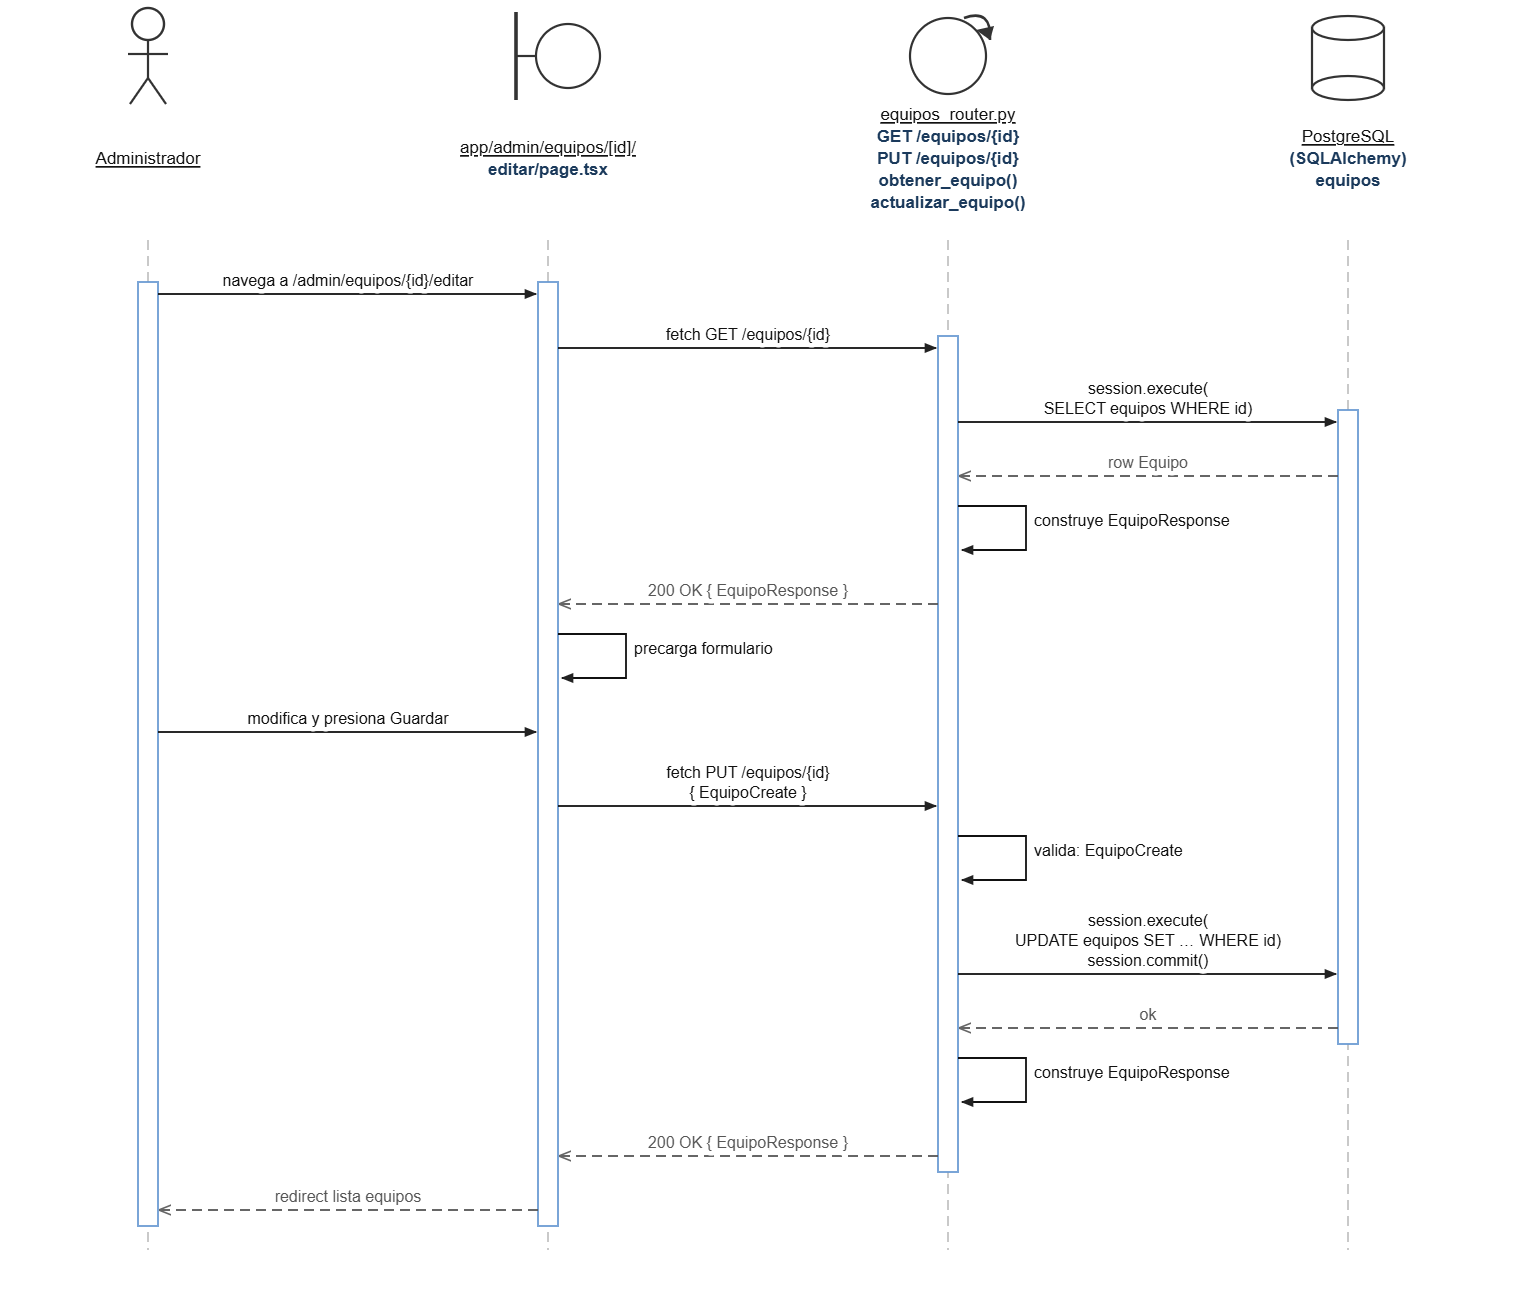
\includegraphics[width=0.8\textwidth]{img/CU-11.png}
	\caption{Diagrama de secuencia --- CU-11 Modificar equipo multidisciplinario.}
	\label{fig:secuencia-cu11}
\end{figure}

\subsection*{Flujo Alternativo / Excepciones}
\begin{itemize}
	\item \textbf{E1: Nombre de equipo duplicado} - El nombre modificado ya existe en otro equipo registrado. El sistema emite un error y bloquea el guardado.
	\item \textbf{E2: Integrantes obligatorios ausentes} - El Administrador intenta guardar el equipo eliminando a todos los miembros de alguna especialidad requerida. El sistema genera un aviso de error detallando la obligatoriedad de contar con al menos un miembro especialista de cada área.
\end{itemize}

\bigskip
\noindent\rule{\linewidth}{0.5pt}
\bigskip

% ============================================================
\section{Diseño Dinámico del CU: Asignar NNA a equipo multidisciplinario (CU-12)}
% ============================================================

\subsection*{Descripción del Flujo}
El Administrador selecciona un NNA del listado de menores y hace clic en "Asignar a equipo". La interfaz solicita la lista de equipos multidisciplinarios activos al Backend. El Administrador selecciona el equipo correspondiente en el menú desplegable y presiona "Confirmar asignación". La interfaz envía el ID del NNA y del equipo al Backend. El Backend valida en la base de datos que el NNA exista y no cuente con una asignación activa actual en otro equipo. Al verificarse, actualiza la tabla de asignaciones asociando al NNA con el equipo multidisciplinario seleccionado en la base de datos. El Backend confirma el éxito de la operación y la interfaz muestra una alerta exitosa.

\begin{figure}[H]
	\centering
	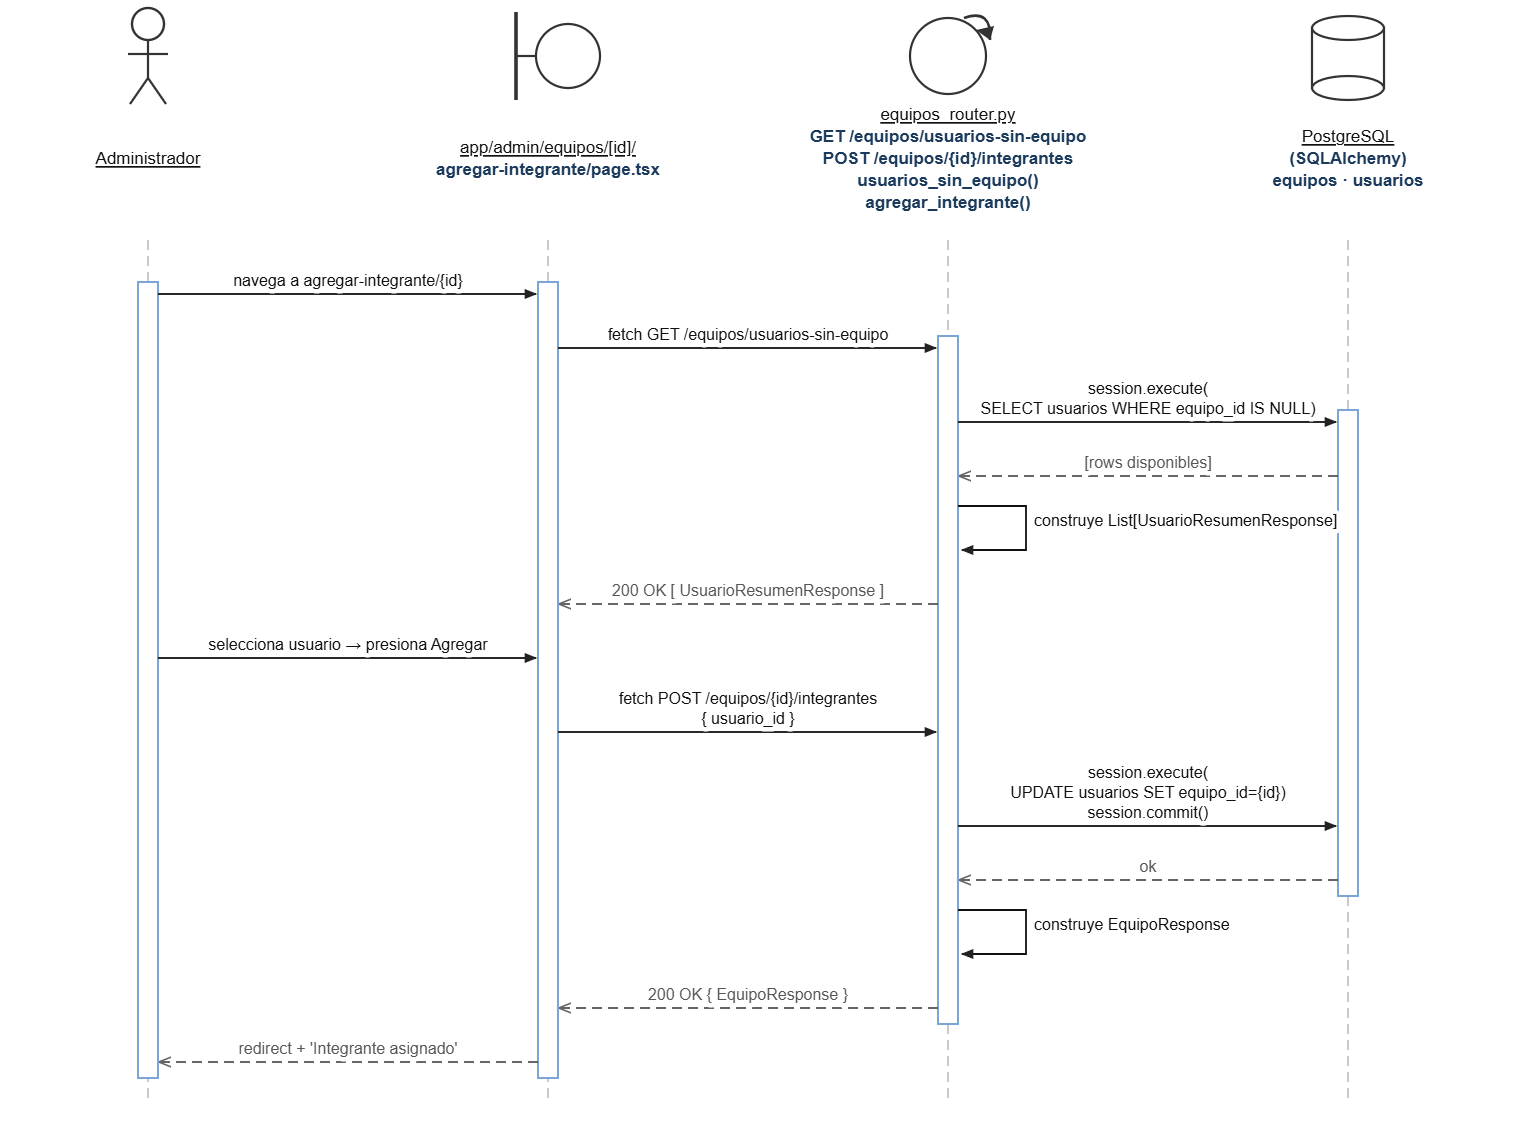
\includegraphics[width=0.8\textwidth]{img/CU-12.png}
	\caption{Diagrama de secuencia --- CU-12 Asignar NNA a equipo multidisciplinario.}
	\label{fig:secuencia-cu12}
\end{figure}

\subsection*{Flujo Alternativo / Excepciones}
\begin{itemize}
	\item \textbf{E1: NNA ya asignado a un equipo activo} - El NNA seleccionado ya tiene una asignación vigente a otro equipo multidisciplinario. El Backend aborta la operación y responde con un mensaje indicando que primero se debe dar de baja al NNA de su equipo actual.
	\item \textbf{E2: Equipo inactivo o inexistente} - Si por algún error de concurrencia el equipo seleccionado es inhabilitado simultáneamente por otro administrador, el sistema aborta la transacción y notifica el error.
\end{itemize}

\bigskip
\noindent\rule{\linewidth}{0.5pt}
\bigskip

% ============================================================
\section{Diseño Dinámico del CU: Registrar NNA (CU-13)}
% ============================================================

\subsection*{Descripción del Flujo}
El Especialista accede al formulario de registro de NNA. Captura los datos generales del menor (nombre, apellidos, CURP, fecha de nacimiento, sexo, escolaridad, idioma) e información de salud (discapacidades y enfermedades). La interfaz realiza las validaciones básicas de campos obligatorios y formato de la CURP. Al guardar, la interfaz envía los datos en formato JSON al Backend. El Backend realiza una validación exhaustiva de los datos y consulta la base de datos para confirmar que la CURP del NNA no esté ya registrada. Si no existe duplicado, inserta el nuevo registro del NNA en la base de datos, asociándole un identificador único y confirmando la inserción. La interfaz de usuario muestra el mensaje de registro exitoso.

\begin{figure}[H]
	\centering
	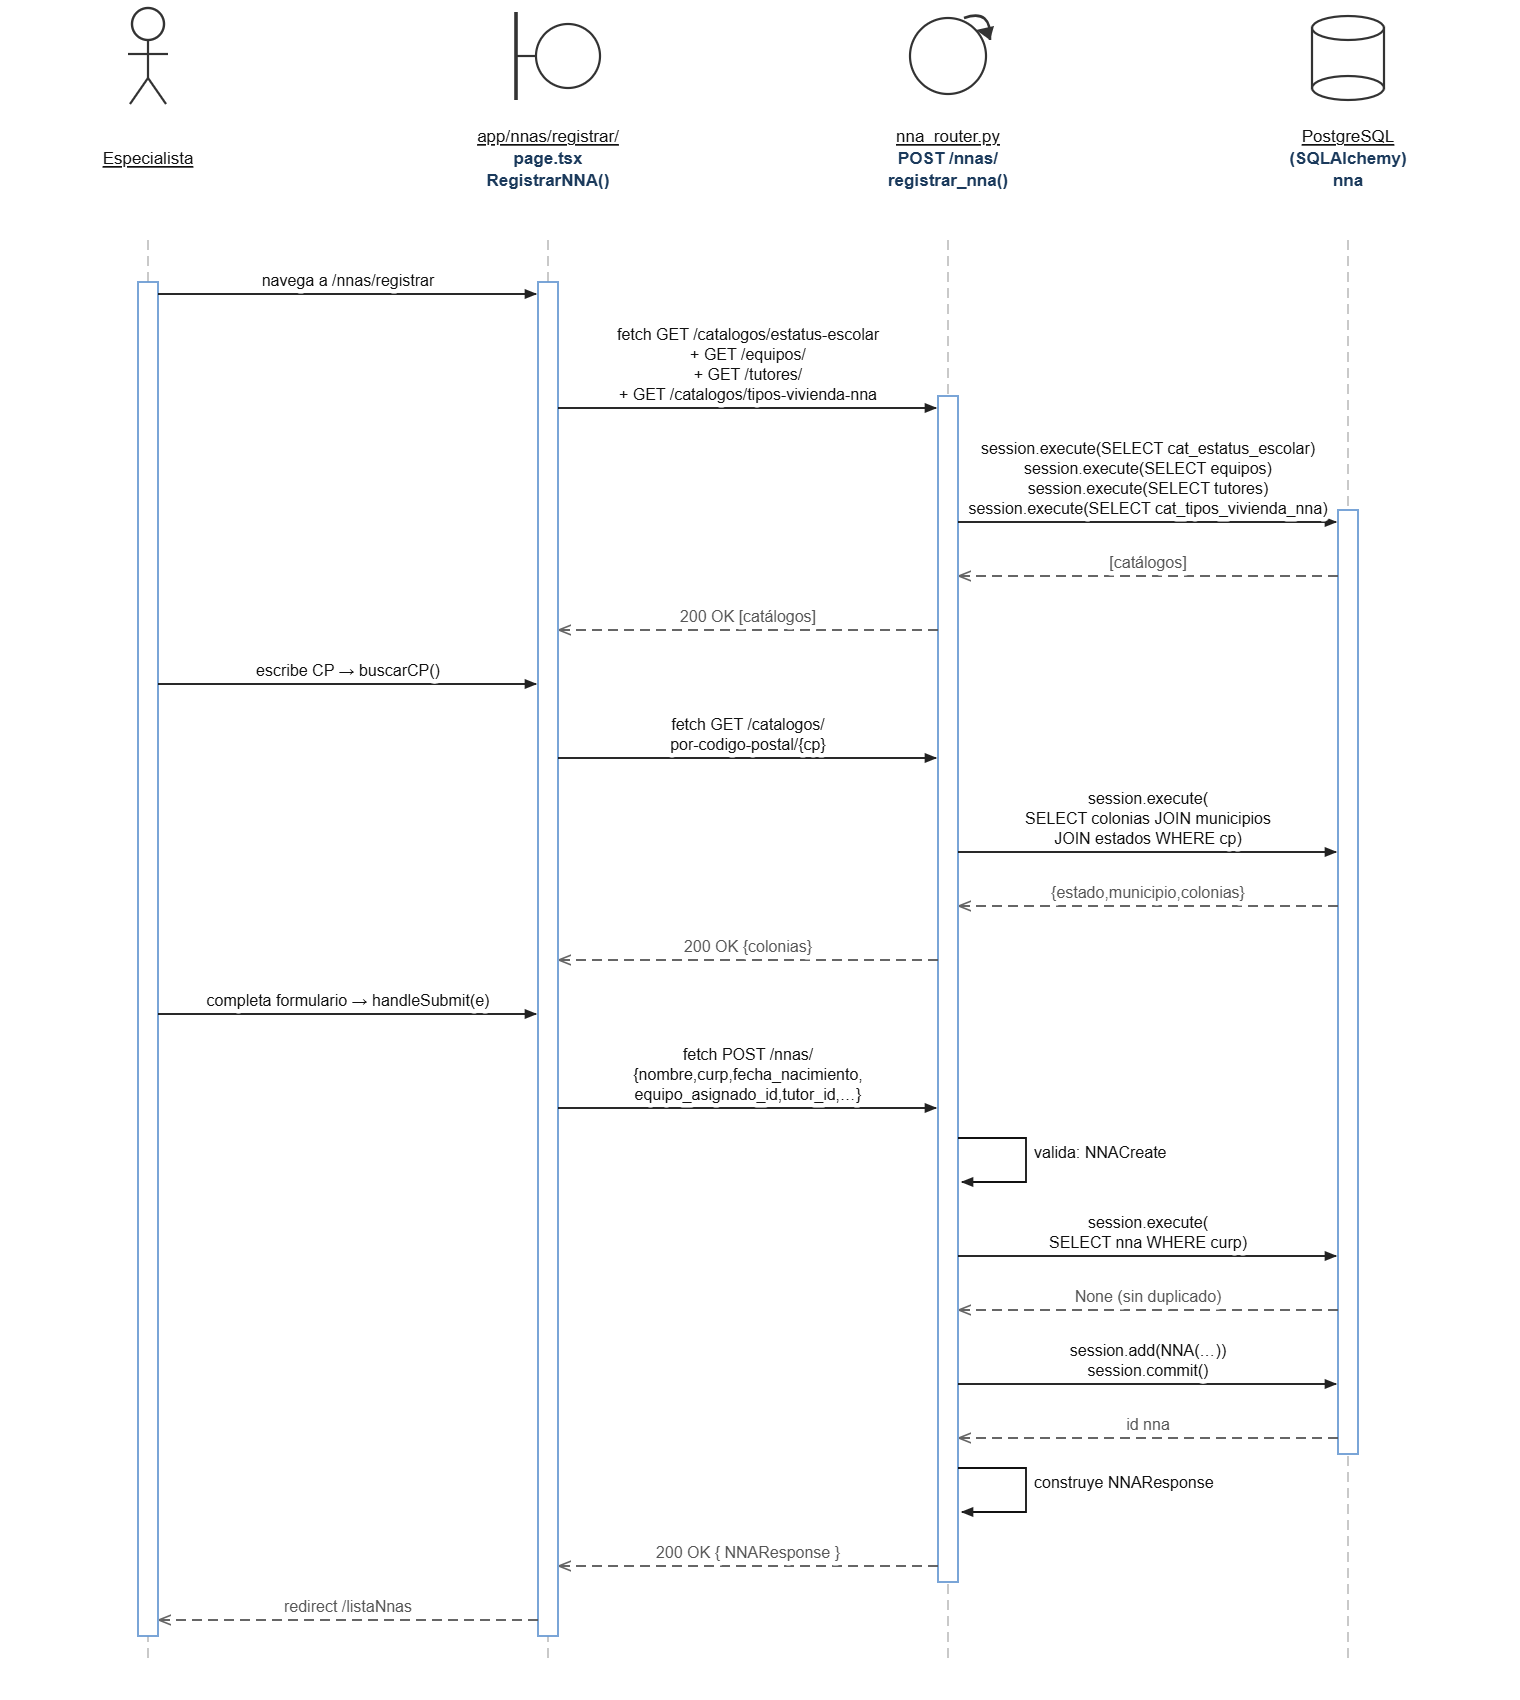
\includegraphics[width=0.8\textwidth]{img/CU-13.png}
	\caption{Diagrama de secuencia --- CU-13 Registrar NNA.}
	\label{fig:secuencia-cu13}
\end{figure}

\subsection*{Flujo Alternativo / Excepciones}
\begin{itemize}
	\item \textbf{E1: CURP del NNA ya registrada} - El sistema detecta en la base de datos que ya existe un menor registrado con la misma CURP. El sistema muestra la advertencia "La CURP ingresada ya existe en el sistema" y detiene la creación.
	\item \textbf{E2: Fecha de nacimiento inválida} - La fecha de nacimiento seleccionada es posterior a la fecha del día de hoy. El sistema muestra un mensaje de error y exige corregir el campo.
	\item \textbf{E3: CURP con formato incorrecto} - Si la CURP no cumple con la longitud de 18 caracteres alfanuméricos válidos, la interfaz de usuario bloquea el envío del formulario.
\end{itemize}

\bigskip
\noindent\rule{\linewidth}{0.5pt}
\bigskip

% ============================================================
\section{Diseño Dinámico del CU: Consultar NNA (CU-14)}
% ============================================================

\subsection*{Descripción del Flujo}
El Especialista ingresa al módulo de NNA y escribe un criterio de búsqueda (nombre completo o CURP) en la barra de consulta. La interfaz envía los términos de búsqueda al Backend. El Backend procesa la solicitud y realiza una consulta con filtros LIKE en la base de datos sobre la tabla de menores. La base de datos retorna el listado de menores que coinciden con la búsqueda. El Backend transmite el listado a la interfaz de usuario, la cual dibuja los resultados en una tabla. El Especialista selecciona a un menor específico y la interfaz carga de forma detallada su ficha de identidad y médica.

\begin{figure}[H]
	\centering
	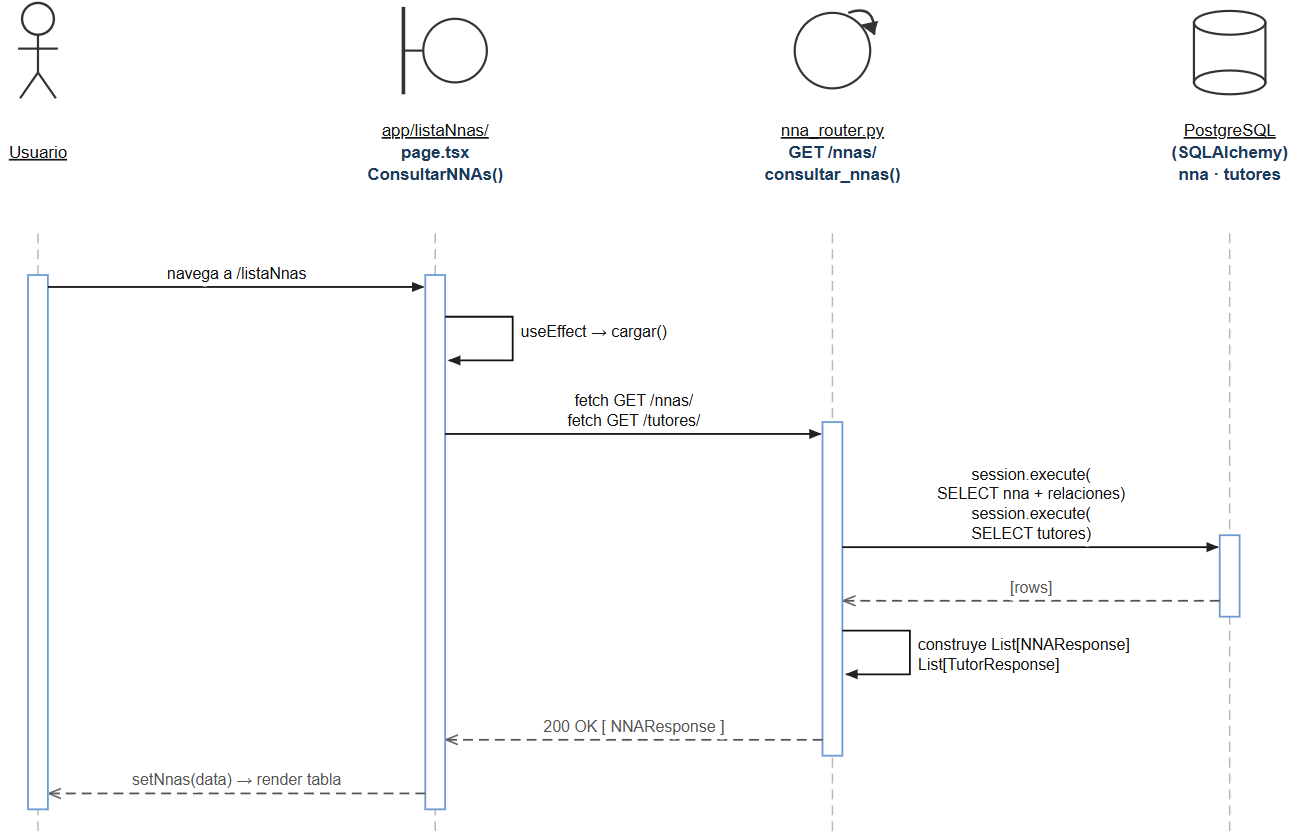
\includegraphics[width=0.8\textwidth]{img/CU14.png}
	\caption{Diagrama de secuencia --- CU-14 Consultar NNA.}
	\label{fig:secuencia-cu14}
\end{figure}

\subsection*{Flujo Alternativo / Excepciones}
\begin{itemize}
	\item \textbf{E1: Sin coincidencias para la búsqueda} - El criterio de búsqueda ingresado no coincide con ningún registro activo en la base de datos. El sistema muestra un aviso de "Sin resultados encontrados" y mantiene la tabla vacía.
\end{itemize}

\bigskip
\noindent\rule{\linewidth}{0.5pt}
\bigskip

% ============================================================
\section{Diseño Dinámico del CU: Modificar datos del NNA (CU-15)}
% ============================================================

\subsection*{Descripción del Flujo}
El Especialista selecciona un NNA y presiona "Modificar datos". La interfaz obtiene los datos actuales del menor del Backend y los despliega en el formulario con opción de edición. El Especialista actualiza la información personal, de escolaridad o de domicilio y pulsa "Guardar cambios". La interfaz envía el conjunto de datos modificados al Backend. El Backend comprueba que los campos obligatorios estén completos y valida que la CURP modificada no esté en uso por otro menor diferente en la base de datos. Tras verificar, aplica las modificaciones en la base de datos y responde éxito. La interfaz de usuario muestra un banner confirmando la actualización.

\begin{figure}[H]
	\centering
	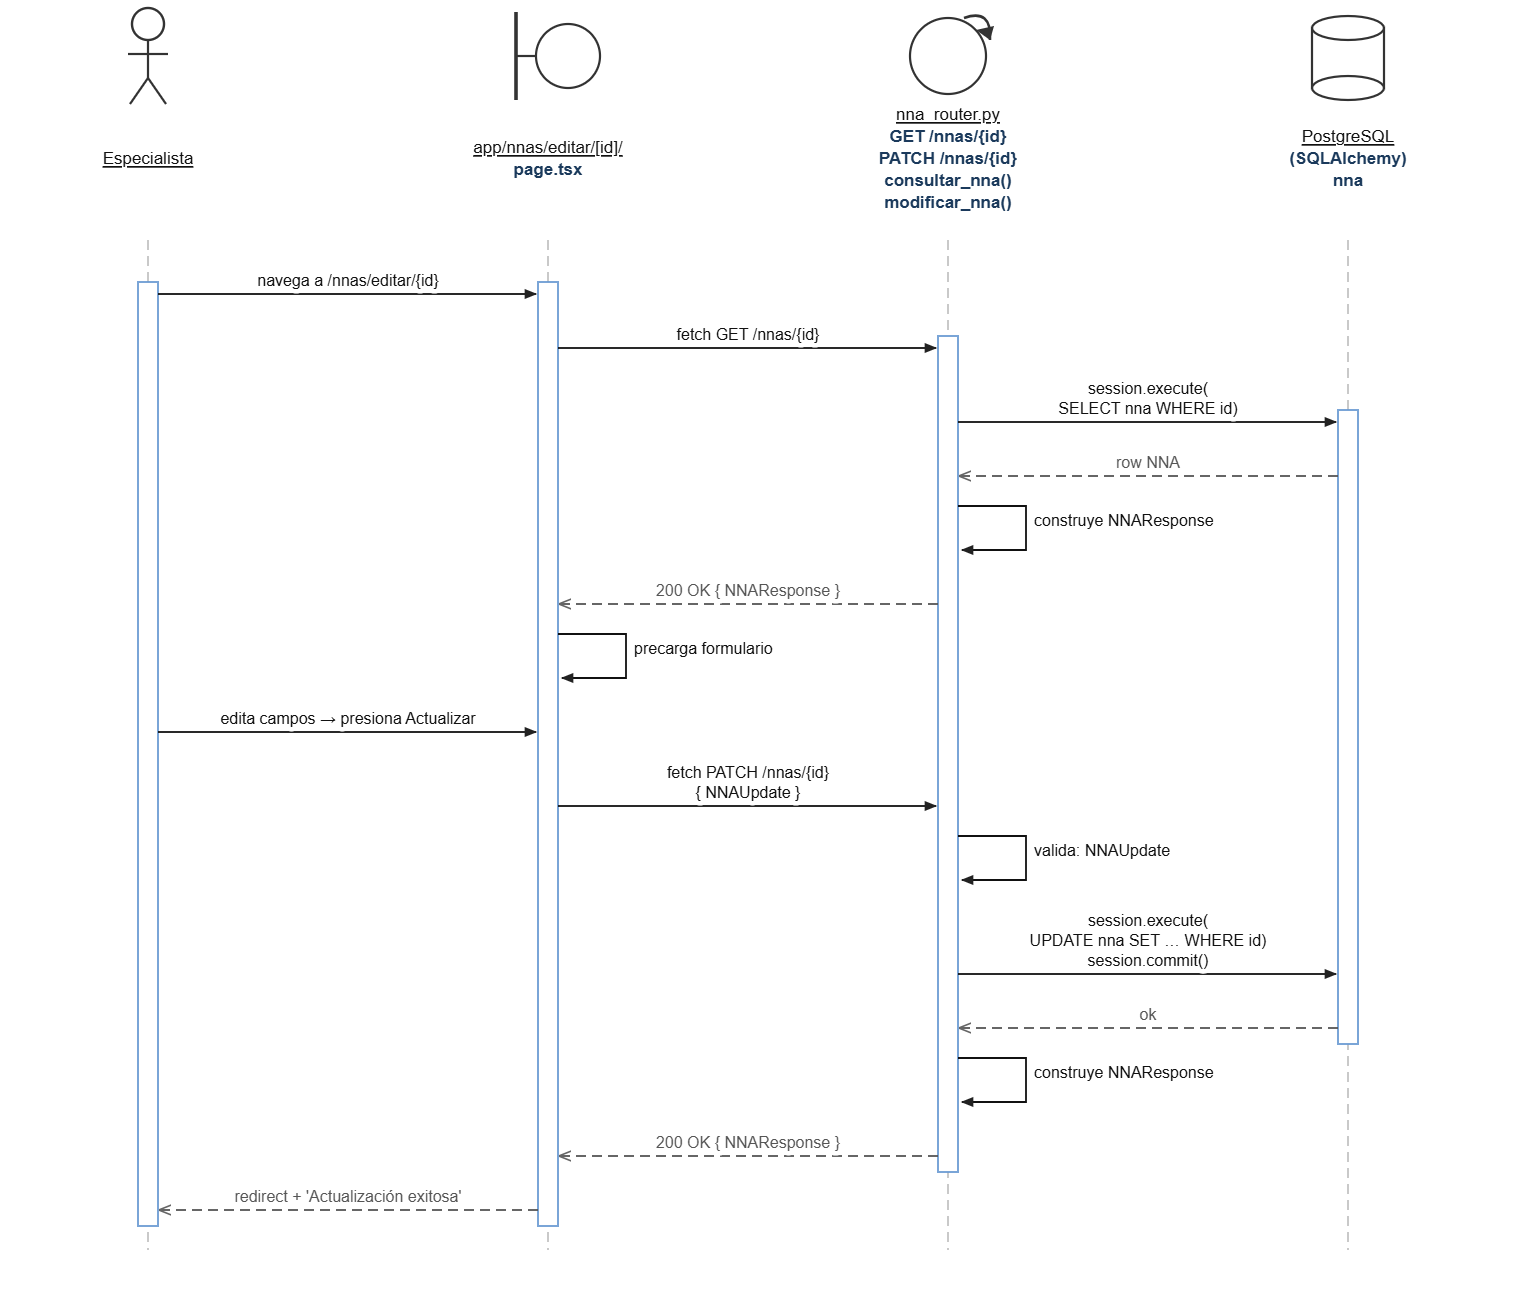
\includegraphics[width=0.8\textwidth]{img/CU-15.png}
	\caption{Diagrama de secuencia --- CU-15 Modificar datos del NNA.}
	\label{fig:secuencia-cu15}
\end{figure}

\subsection*{Flujo Alternativo / Excepciones}
\begin{itemize}
	\item \textbf{E1: CURP del NNA duplicada} - La CURP modificada colisiona con el registro de otro menor en la base de datos. El sistema interrumpe el proceso de actualización y devuelve un error.
	\item \textbf{E2: Datos obligatorios en blanco} - El usuario borra información obligatoria (como el nombre o la fecha de nacimiento). La interfaz impide el guardado y resalta las anomalías.
\end{itemize}

\bigskip
\noindent\rule{\linewidth}{0.5pt}
\bigskip

% ============================================================
\section{Diseño Dinámico del CU: Registrar hecho victimal (CU-16)}
% ============================================================

\subsection*{Descripción del Flujo}
El Especialista ingresa a la pestaña de Hechos Victimales dentro del expediente de un NNA. Selecciona "Añadir hecho victimal" e ingresa la información requerida: fecha y hora del hecho, descripción detallada, lugar del suceso, y tipo de vulneración o violencia (psicológica, física, negligencia, etc.). La interfaz valida la completitud de los datos. Al presionar "Guardar", la solicitud es enviada al Backend. El Backend comprueba que la fecha del hecho sea válida (no posterior a la actual y posterior al nacimiento del menor) y registra el hecho victimal asociado al NNA en la base de datos. El sistema devuelve el éxito de la operación y actualiza la cronología del expediente del NNA.

\begin{figure}[H]
	\centering
	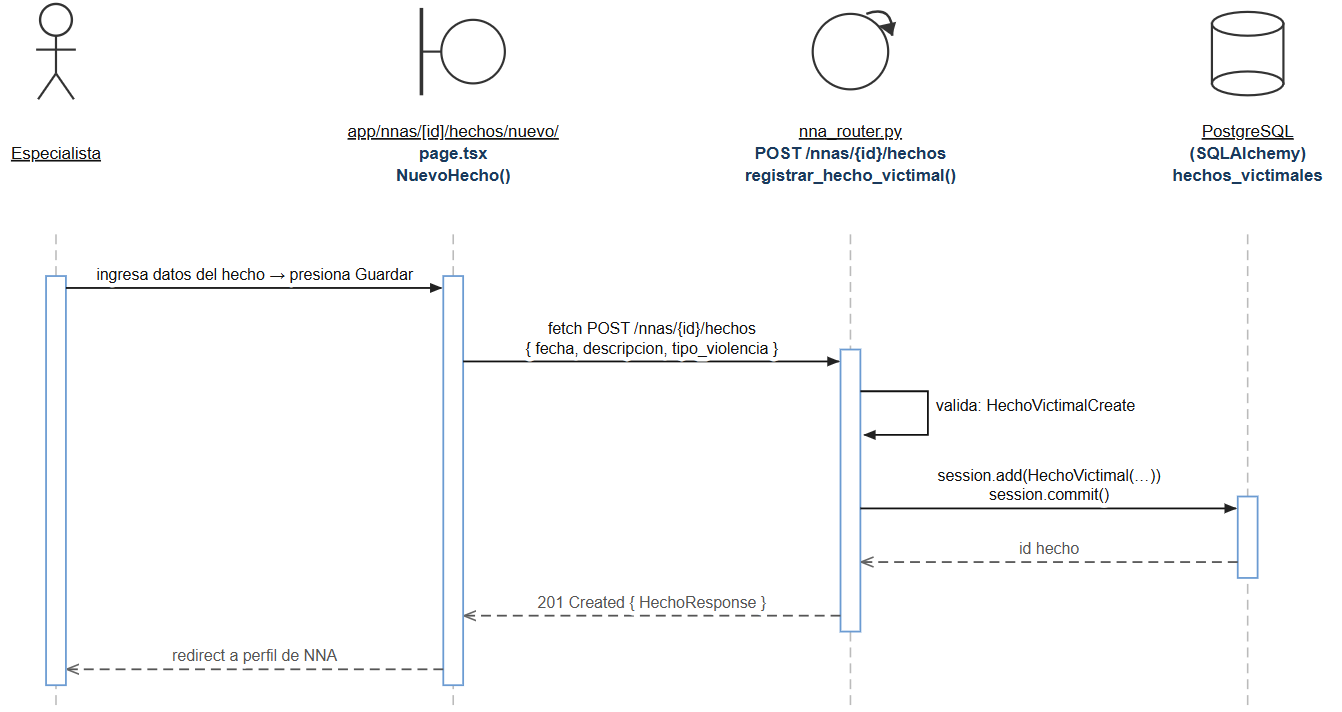
\includegraphics[width=0.8\textwidth]{img/CU16.png}
	\caption{Diagrama de secuencia --- CU-16 Registrar hecho victimal.}
	\label{fig:secuencia-cu16}
\end{figure}

\subsection*{Flujo Alternativo / Excepciones}
\begin{itemize}
	\item \textbf{E1: Campos obligatorios incompletos} - Se intenta guardar el registro omitiendo la descripción o el tipo de hecho victimal. El sistema detiene la transacción e indica los errores en la pantalla.
	\item \textbf{E2: Fecha del hecho victimal inválida} - La fecha ingresada es futura o anterior al nacimiento del NNA. Se emite un aviso de incongruencia de fechas y regresa al formulario.
\end{itemize}

\bigskip
\noindent\rule{\linewidth}{0.5pt}
\bigskip

% ============================================================
\section{Diseño Dinámico del CU: Modificar hecho victimal (CU-17)}
% ============================================================

\subsection*{Descripción del Flujo}
El Especialista localiza un hecho victimal en la línea del tiempo del NNA y presiona "Editar". La interfaz carga el formulario con los datos registrados y habilitados para cambios. El Especialista edita la descripción, la fecha o el tipo de hecho y presiona "Actualizar". El Backend recibe la solicitud, valida la fecha y aplica la actualización sobre el registro del hecho victimal en la base de datos. Finalmente, retorna una respuesta exitosa, actualizando la línea del tiempo en el expediente.

\begin{figure}[H]
	\centering
	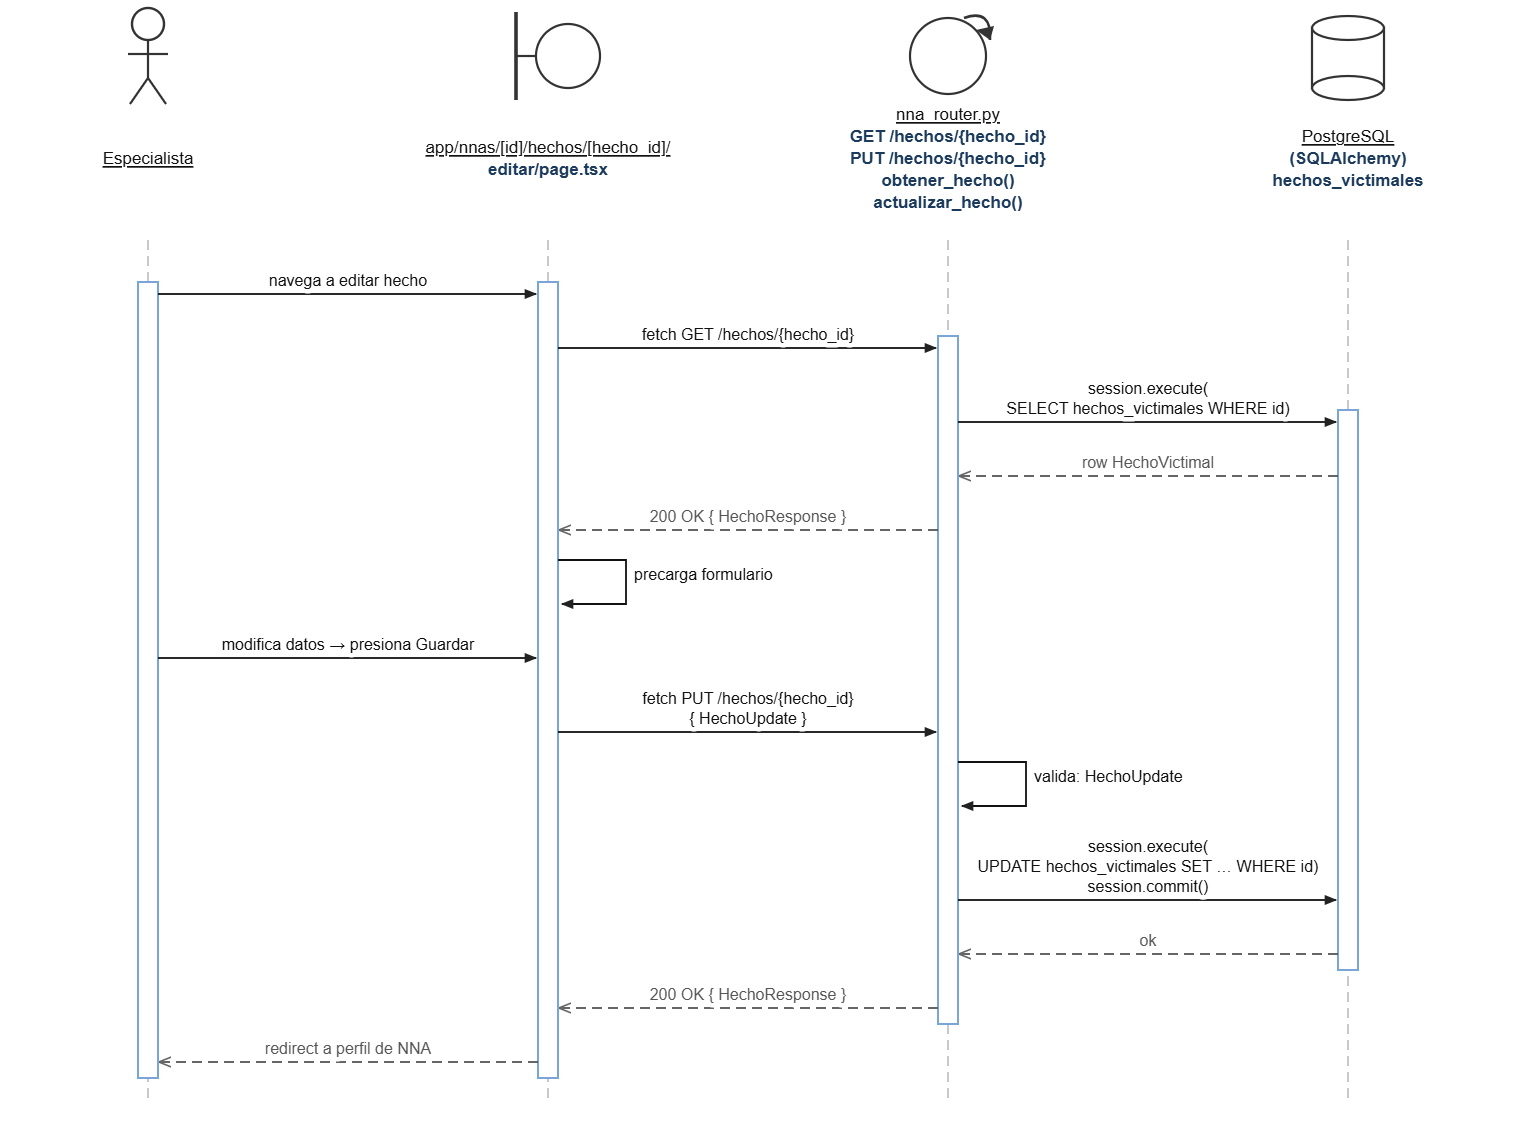
\includegraphics[width=0.8\textwidth]{img/CU-17.png}
	\caption{Diagrama de secuencia --- CU-17 Modificar hecho victimal.}
	\label{fig:secuencia-cu17}
\end{figure}

\subsection*{Flujo Alternativo / Excepciones}
\begin{itemize}
	\item \textbf{E1: Identificador del hecho victimal inexistente} - Si por problemas de concurrencia el registro a editar fue eliminado previamente, el sistema devuelve un error indicando que el hecho ya no existe en el sistema.
	\item \textbf{E2: Fecha del hecho no válida} - Si la fecha modificada entra en conflicto con las fechas del menor, se cancela la edición y se muestra una alerta.
\end{itemize}

\bigskip
\noindent\rule{\linewidth}{0.5pt}
\bigskip

% ============================================================
\section{Diseño Dinámico del CU: Registrar tutor del NNA (CU-18)}
% ============================================================

\subsection*{Descripción del Flujo}
El Especialista accede a la sección de tutores dentro del perfil de un NNA. Selecciona "Registrar Tutor" y completa el formulario con los datos de identidad (nombre, parentesco, CURP, fecha de nacimiento, ocupación, escolaridad) y domicilio del tutor. Al presionar "Guardar", la interfaz envía los datos al Backend. El Backend verifica en la base de datos que la CURP del tutor sea única. Al validarse la información, crea el registro del tutor en la base de datos y establece la relación de tutoría con el NNA. El Backend confirma el registro exitoso a la interfaz, que actualiza la sección de familiares del menor.

\begin{figure}[H]
	\centering
	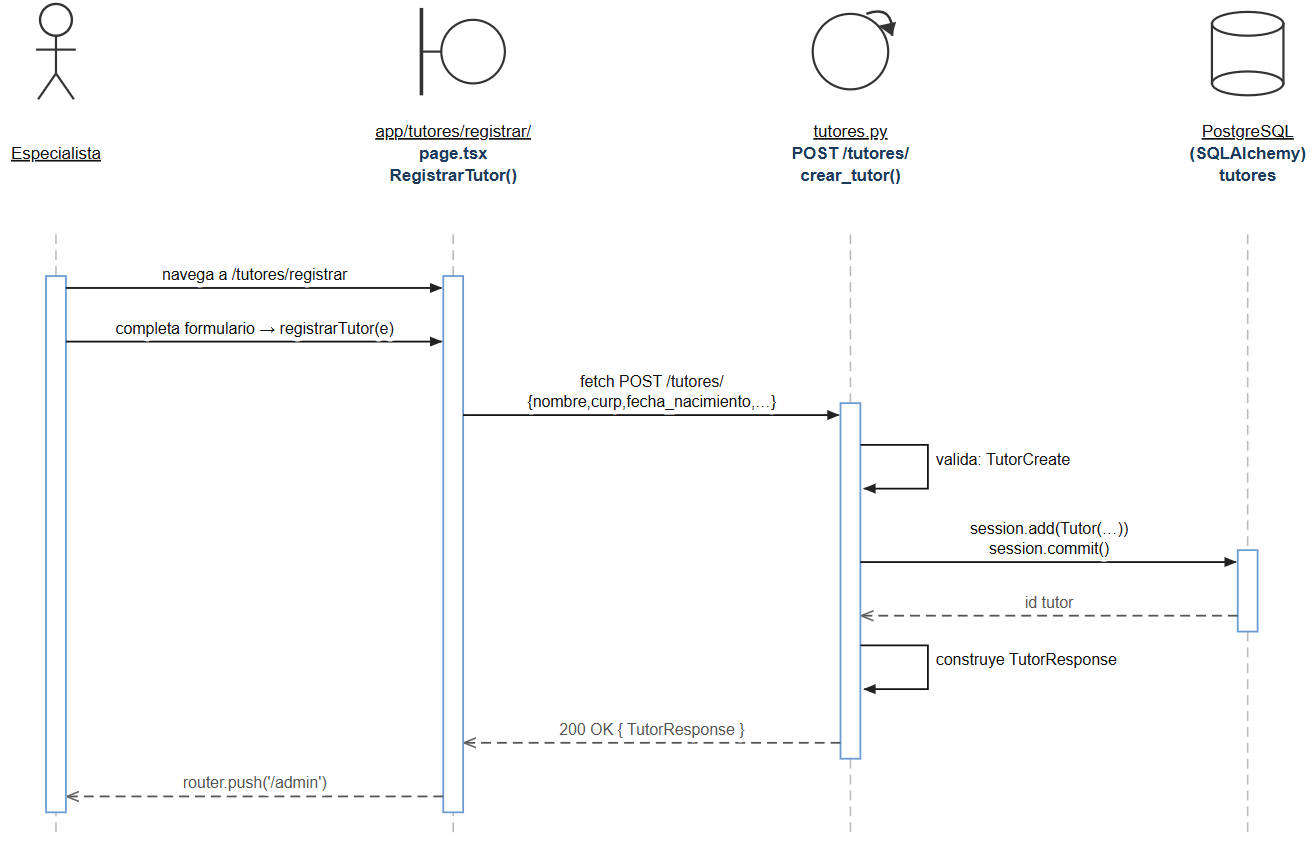
\includegraphics[width=0.8\textwidth]{img/CU18.png}
	\caption{Diagrama de secuencia --- CU-18 Registrar tutor del NNA.}
	\label{fig:secuencia-cu18}
\end{figure}

\subsection*{Flujo Alternativo / Excepciones}
\begin{itemize}
	\item \textbf{E1: CURP del tutor ya registrada} - La CURP del tutor ya se encuentra en la base de datos asociada a otra persona. El sistema muestra la advertencia "El tutor con esta CURP ya está registrado" y permite buscarlo para asociarlo.
	\item \textbf{E2: Edad inconsistente del tutor} - La fecha de nacimiento indica que el tutor es menor de edad. El sistema rechaza el registro por no cumplir el requisito legal de mayoría de edad.
\end{itemize}

\bigskip
\noindent\rule{\linewidth}{0.5pt}
\bigskip

% ============================================================
\section{Diseño Dinámico del CU: Modificar datos del tutor (CU-19)}
% ============================================================

\subsection*{Descripción del Flujo}
El Especialista selecciona al tutor en la ficha del NNA y hace clic en "Editar datos del tutor". La interfaz presenta los datos actuales en el formulario editable. El Especialista actualiza la información (teléfono, domicilio, estado civil) y presiona "Guardar". El Backend valida los datos modificados y comprueba que la CURP modificada no genere conflictos de duplicidad. Posteriormente, guarda los cambios en el registro del tutor en la base de datos y responde con confirmación a la interfaz.

\begin{figure}[H]
	\centering
	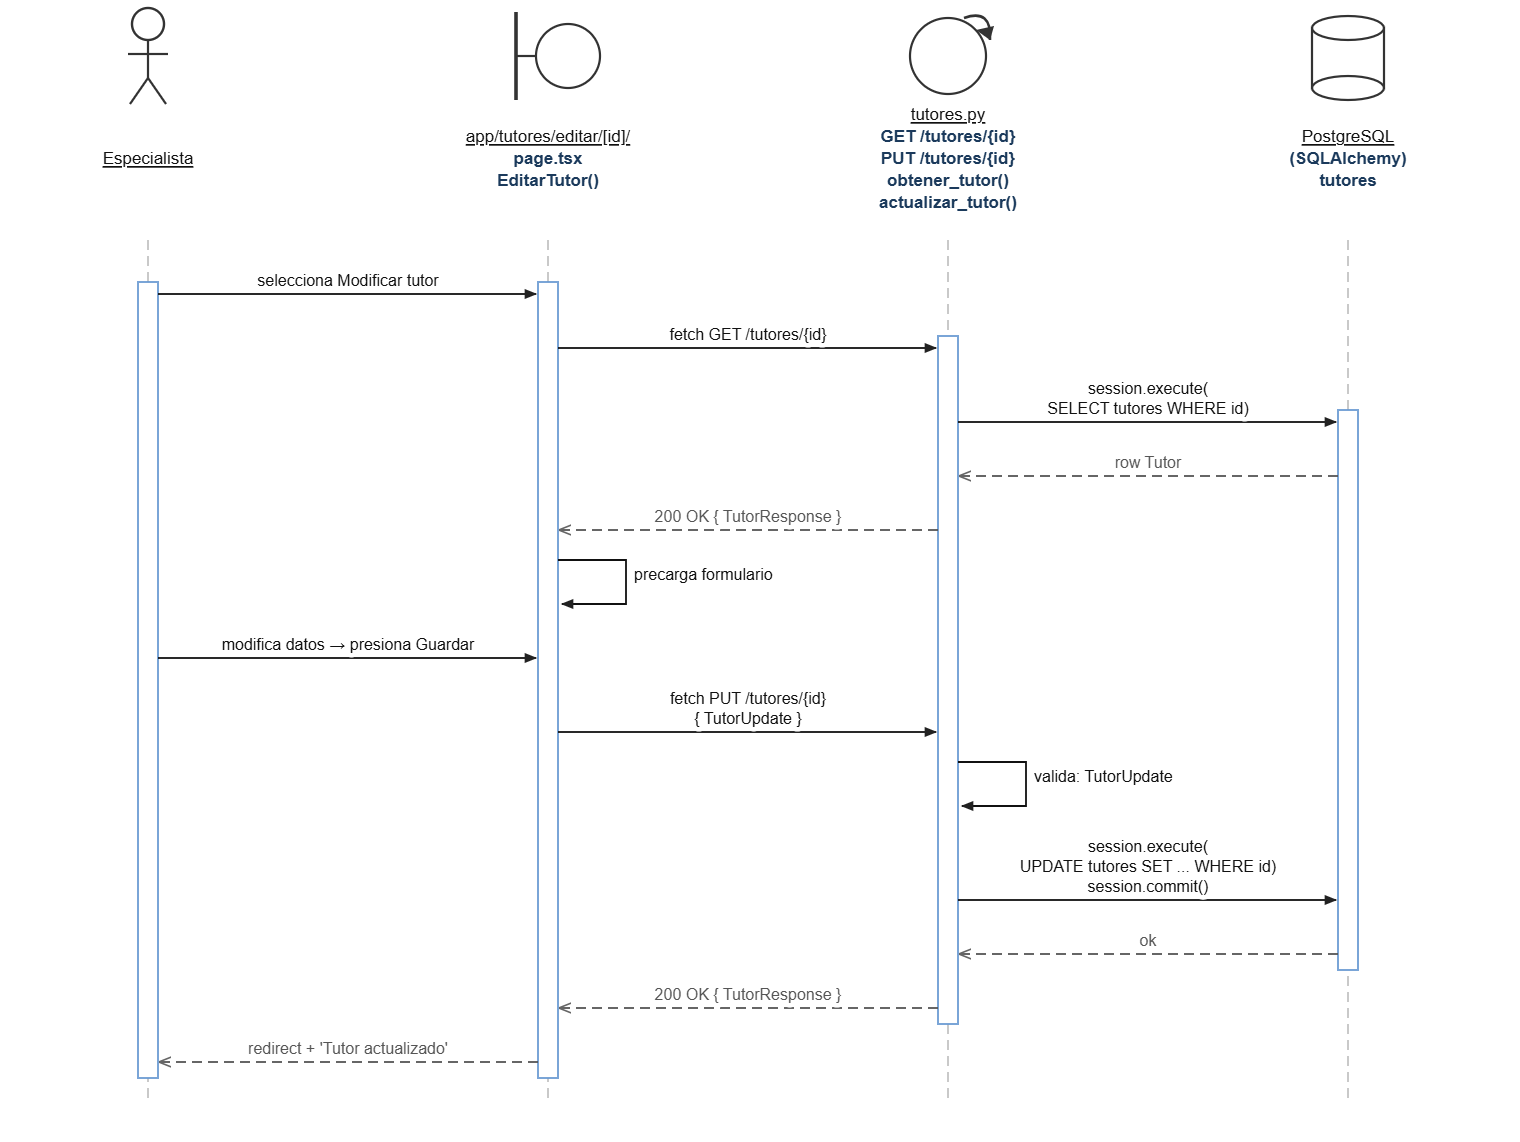
\includegraphics[width=0.8\textwidth]{img/CU-19.png}
	\caption{Diagrama de secuencia --- CU-19 Modificar datos del tutor.}
	\label{fig:secuencia-cu19}
\end{figure}

\subsection*{Flujo Alternativo / Excepciones}
\begin{itemize}
	\item \textbf{E1: CURP modificada duplicada} - La CURP alterada ya pertenece a otro tutor registrado en el sistema. El Backend rechaza la modificación y se muestra una alerta en pantalla.
	\item \textbf{E2: Campos obligatorios vacíos} - Si el usuario vacía campos esenciales, el sistema impide guardar y marca el error visualmente.
\end{itemize}

\bigskip
\noindent\rule{\linewidth}{0.5pt}
\bigskip

% ============================================================
\section{Diseño Dinámico del CU: Abrir expediente (CU-20)}
% ============================================================

\subsection*{Descripción del Flujo}
El Especialista localiza a un NNA que no tiene una atención activa e inicia el trámite de apertura de expediente. Introduce el motivo de apertura (abandono, maltrato, etc.), el Especialista a cargo y el estado inicial del caso. Al pulsar "Abrir Expediente", la interfaz envía la información al Backend. El Backend realiza una consulta en la base de datos para confirmar que el NNA no tenga ya un expediente con estado "Abierto". Al confirmarse la ausencia de duplicados, el Backend genera un identificador único de expediente (siguiendo el formato institucional), registra el expediente en la base de datos y asocia al NNA. El sistema devuelve el número del expediente y abre su vista de administración de caso.

\begin{figure}[H]
	\centering
	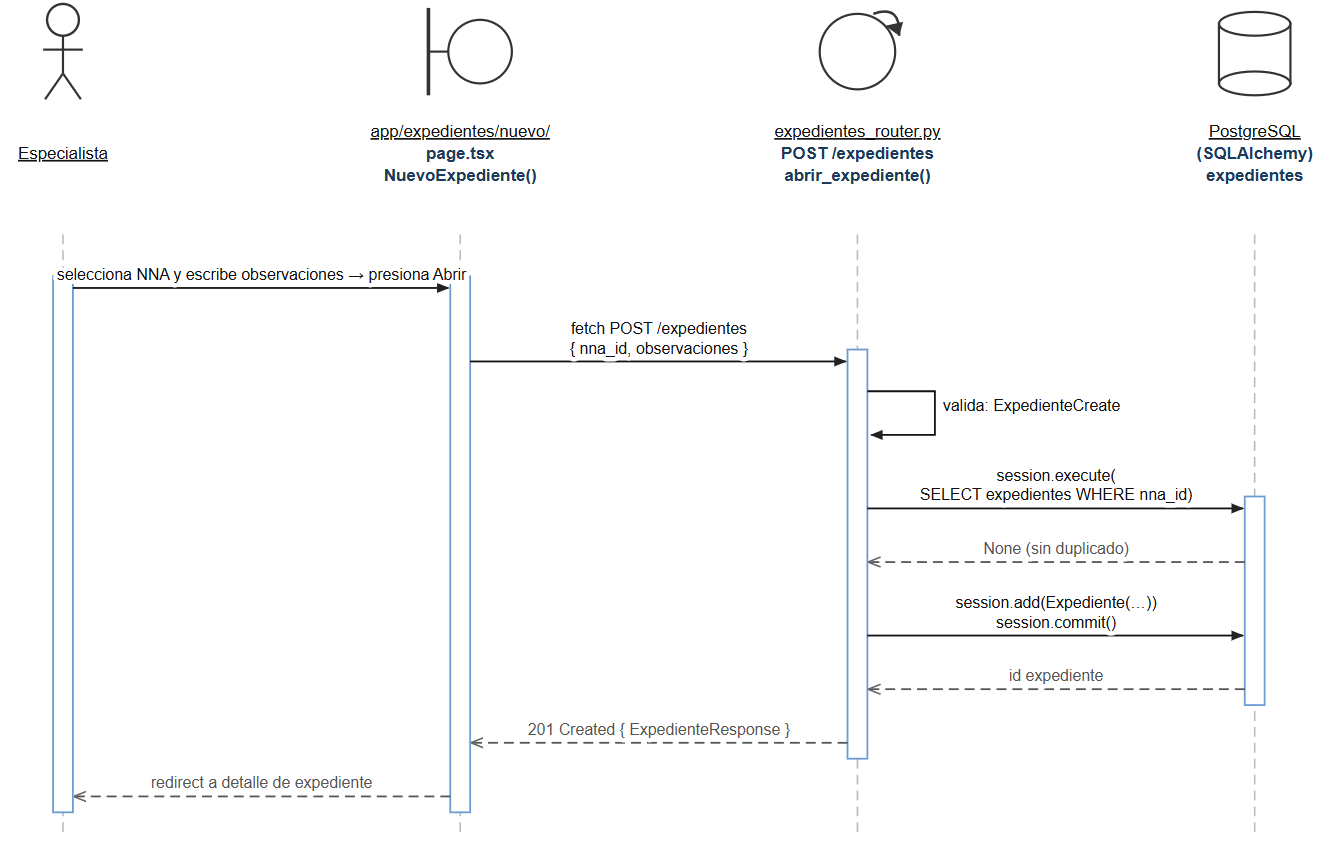
\includegraphics[width=0.8\textwidth]{img/CU20.png}
	\caption{Diagrama de secuencia --- CU-20 Abrir expediente.}
	\label{fig:secuencia-cu20}
\end{figure}

\subsection*{Flujo Alternativo / Excepciones}
\begin{itemize}
	\item \textbf{E1: El NNA ya cuenta con un expediente abierto} - El menor seleccionado ya posee un proceso de atención vigente. El sistema deniega la creación de un nuevo expediente y muestra la alerta "El NNA ya tiene un expediente abierto".
\end{itemize}

\bigskip
\noindent\rule{\linewidth}{0.5pt}
\bigskip

% ============================================================
\section{Diseño Dinámico del CU: Consultar expediente (CU-21)}
% ============================================================

\subsection*{Descripción del Flujo}
El Especialista introduce el número de expediente o busca al NNA en la interfaz de casos de atención. Al seleccionar el registro, la interfaz solicita la información consolidada al Backend. El Backend ejecuta múltiples consultas select parametrizadas en la base de datos para reunir: la ficha del NNA, los datos de su tutor, los hechos victimales, la lista de valoraciones multidisciplinarias (psicológica, médica, de trabajo social) y los derechos vulnerados detectados. El Backend estructura estos datos y los envía a la interfaz, que renderiza la vista unificada del expediente de manera cronológica.

\begin{figure}[H]
	\centering
	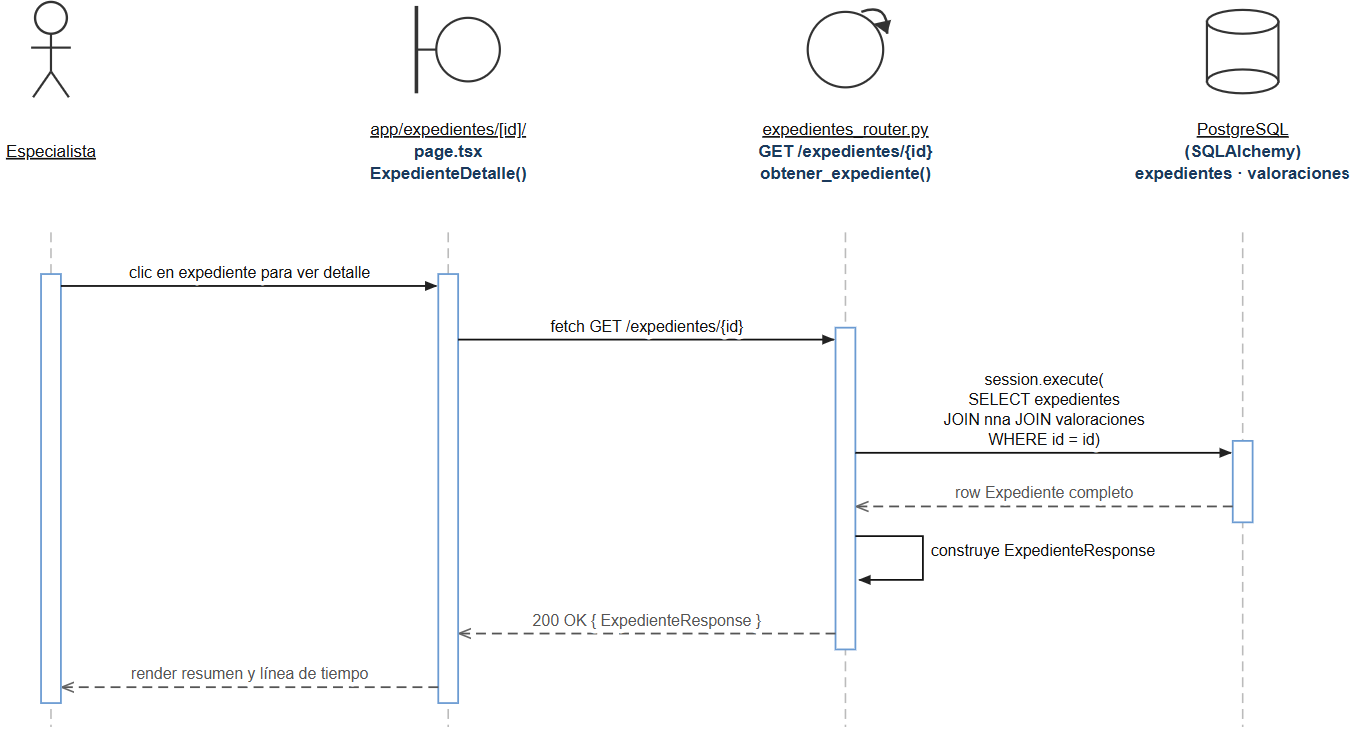
\includegraphics[width=0.8\textwidth]{img/CU21.png}
	\caption{Diagrama de secuencia --- CU-21 Consultar expediente.}
	\label{fig:secuencia-cu21}
\end{figure}

\subsection*{Flujo Alternativo / Excepciones}
\begin{itemize}
	\item \textbf{E1: Expediente no encontrado} - El número de expediente ingresado no corresponde a ningún registro en el sistema. Se muestra el aviso "Expediente inexistente".
	\item \textbf{E2: Acceso restringido} - El Especialista que intenta consultar no pertenece al equipo multidisciplinario asignado a ese caso ni posee un rol de Administrador. El Backend deniega la información y la interfaz muestra "Acceso no autorizado al expediente".
\end{itemize}

\bigskip
\noindent\rule{\linewidth}{0.5pt}
\bigskip

% ============================================================
\section{Diseño Dinámico del CU: Registrar valoración multidisciplinaria (CU-22)}
% ============================================================

\subsection*{Descripción del Flujo}
El Especialista de un área de atención (Psicología, Trabajo Social o Medicina) ingresa a la sección de valoraciones del expediente del NNA y selecciona "Nueva valoración". Selecciona su especialidad, añade la fecha de la valoración, el diagnóstico clínico u observaciones detalladas, y sube un documento de respaldo si es necesario. Al guardar, la interfaz envía los datos al Backend. El Backend valida que el expediente esté abierto y guarda el registro de la valoración multidisciplinaria asociado al expediente en la base de datos. El Backend responde de manera exitosa y la interfaz actualiza la sección de diagnósticos del expediente.

\begin{figure}[H]
	\centering
	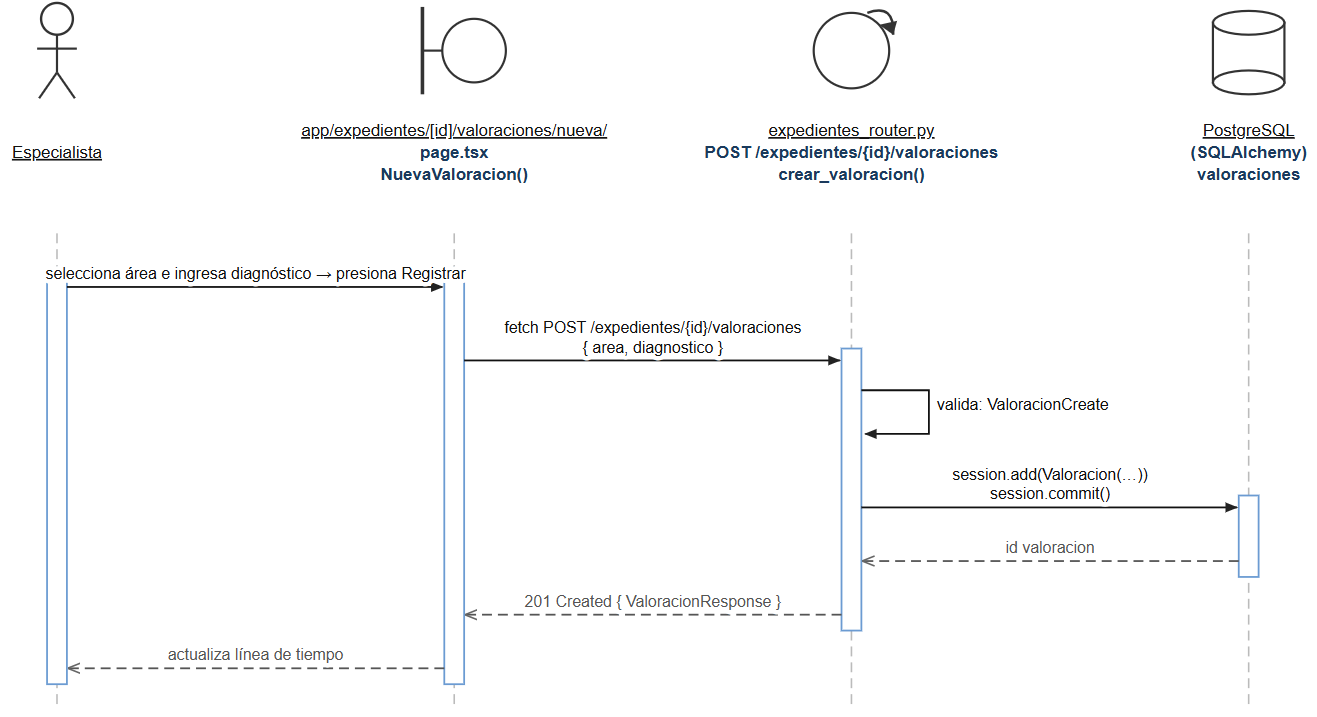
\includegraphics[width=0.8\textwidth]{img/CU22.png}
	\caption{Diagrama de secuencia --- CU-22 Registrar valoración multidisciplinaria.}
	\label{fig:secuencia-cu22}
\end{figure}

\subsection*{Flujo Alternativo / Excepciones}
\begin{itemize}
	\item \textbf{E1: Campos obligatorios incompletos} - Si se intenta guardar la valoración sin agregar el diagnóstico o el campo de área. El sistema bloquea el guardado e indica las omisiones.
	\item \textbf{E2: Expediente inactivo o cerrado} - Se intenta registrar la valoración en un expediente archivado o cerrado. El Backend rechaza el guardado debido a que no se permiten adiciones a expedientes cerrados.
\end{itemize}

\bigskip
\noindent\rule{\linewidth}{0.5pt}
\bigskip

% ============================================================
\section{Diseño Dinámico del CU: Modificar valoración multidisciplinaria (CU-23)}
% ============================================================

\subsection*{Descripción del Flujo}
El Especialista que realizó la valoración la localiza en el listado del expediente y presiona "Modificar". La interfaz muestra la valoración en el formulario de edición. El Especialista modifica los campos permitidos (diagnóstico, recomendaciones u observaciones) y presiona "Actualizar". El Backend valida que el Especialista sea el autor de la valoración (o posea los permisos necesarios) y que el expediente siga abierto. Si es correcto, actualiza el registro en la base de datos y devuelve éxito. La interfaz actualiza la vista del expediente.

\begin{figure}[H]
	\centering
	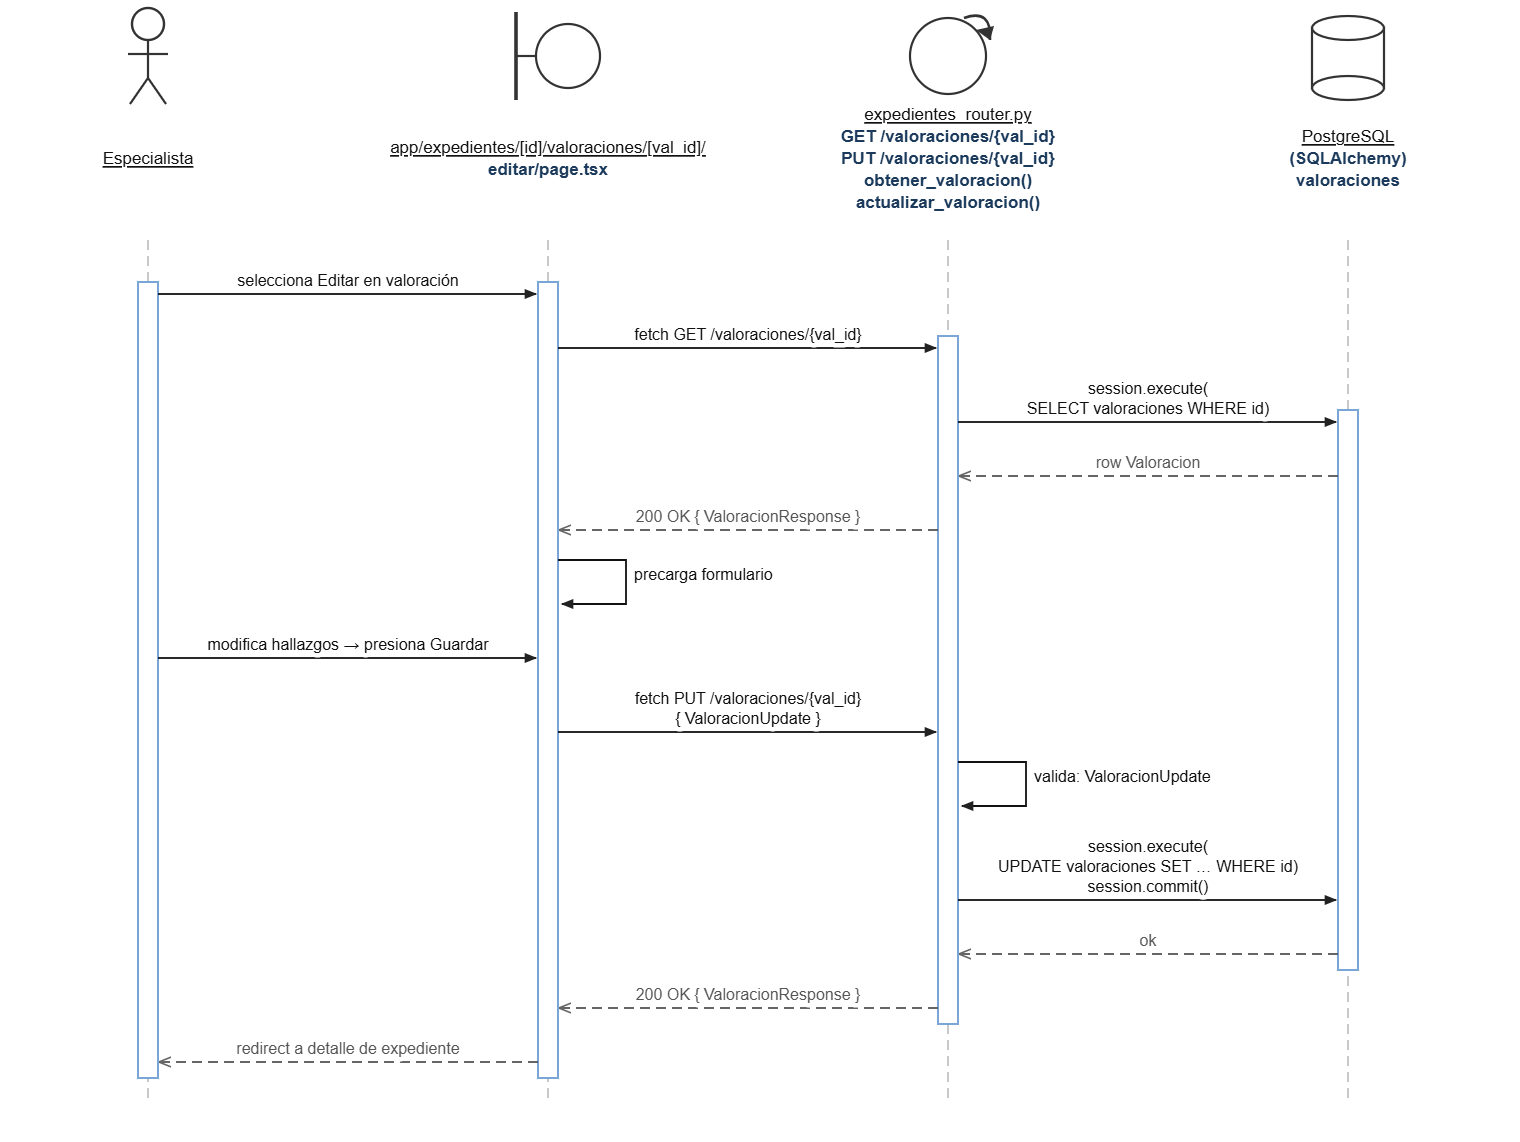
\includegraphics[width=0.8\textwidth]{img/CU-23.png}
	\caption{Diagrama de secuencia --- CU-23 Modificar valoración multidisciplinaria.}
	\label{fig:secuencia-cu23}
\end{figure}

\subsection*{Flujo Alternativo / Excepciones}
\begin{itemize}
	\item \textbf{E1: Valoración no encontrada} - El identificador de la valoración a modificar ya no existe en la base de datos.
	\item \textbf{E2: Intento de edición por otro usuario} - Un especialista diferente al autor original intenta modificar la valoración. El Backend bloquea la edición por seguridad y muestra el error "No tiene permisos para modificar esta valoración".
\end{itemize}

\bigskip
\noindent\rule{\linewidth}{0.5pt}
\bigskip

% ============================================================
\section{Diseño Dinámico del CU: Registrar derecho vulnerado (CU-24)}
% ============================================================

\subsection*{Descripción del Flujo}
El Especialista ingresa al módulo de derechos del NNA en su expediente y presiona "Registrar vulneración". Selecciona un derecho de la lista oficial de derechos de los NNA (LGDNNA) y añade una descripción de las circunstancias detectadas de la vulneración. Al guardar, la interfaz envía la información al Backend. El Backend verifica en la base de datos que el derecho seleccionado exista y no esté ya registrado previamente como vulnerado y vigente en el mismo expediente. Si cumple, inserta la vulneración del derecho en la base de datos vinculada al expediente y retorna éxito. La interfaz actualiza el cuadro de derechos vulnerados.

\begin{figure}[H]
	\centering
	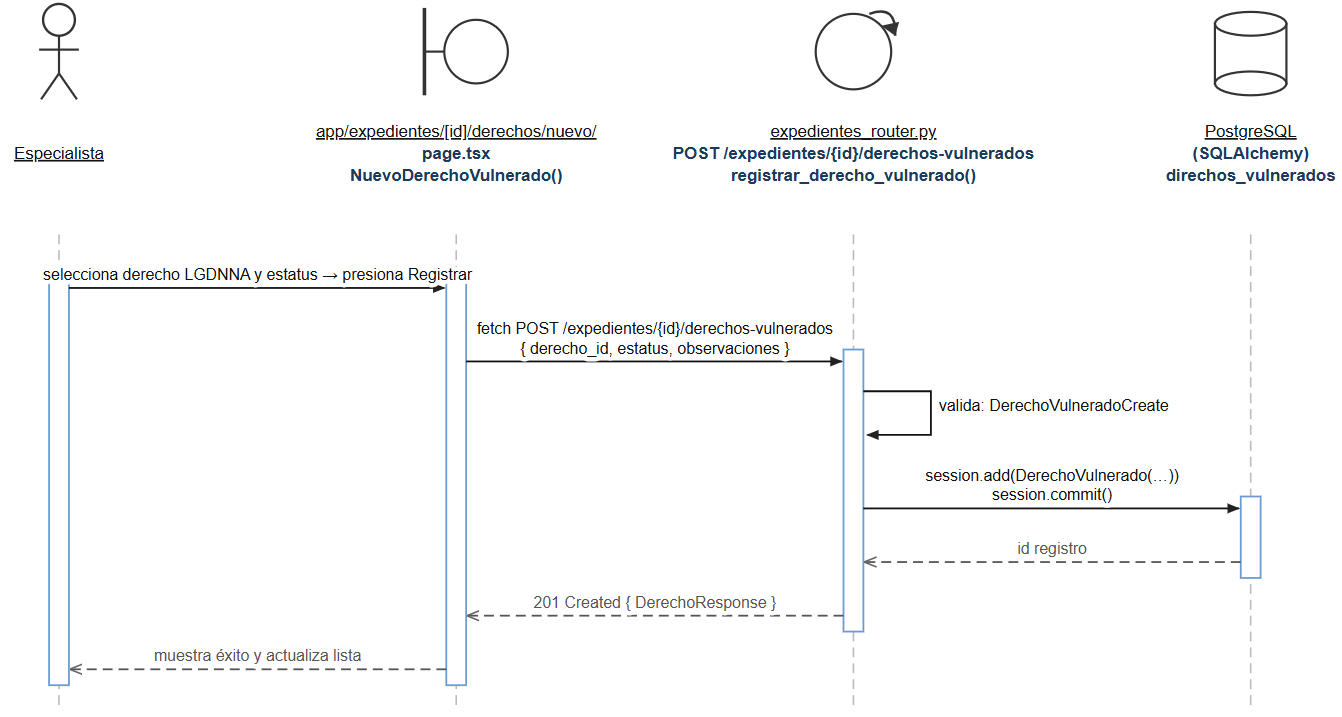
\includegraphics[width=0.8\textwidth]{img/CU24.png}
	\caption{Diagrama de secuencia --- CU-24 Registrar derecho vulnerado.}
	\label{fig:secuencia-cu24}
\end{figure}

\subsection*{Flujo Alternativo / Excepciones}
\begin{itemize}
	\item \textbf{E1: Derecho ya registrado en el expediente} - El derecho que se intenta agregar ya se encuentra listado como vulnerado en el expediente activo del NNA. El sistema despliega el mensaje "Este derecho ya se encuentra registrado como vulnerado" y aborta la transacción.
\end{itemize}

\bigskip
\noindent\rule{\linewidth}{0.5pt}
\bigskip

% ============================================================
\section{Diseño Dinámico del CU: Modificar derecho vulnerado (CU-25)}
% ============================================================

\subsection*{Descripción del Flujo}
El Especialista selecciona un derecho vulnerado registrado en el expediente y hace clic en "Actualizar estado". Modifica el estado del derecho (por ejemplo, a "Restituido") e ingresa las medidas de restitución tomadas y las observaciones de seguimiento. La interfaz envía los datos actualizados al Backend. El Backend valida la existencia del registro, actualiza el estado y las observaciones del derecho en la base de datos y devuelve éxito. La interfaz actualiza el indicador de derechos del menor.

\begin{figure}[H]
	\centering
	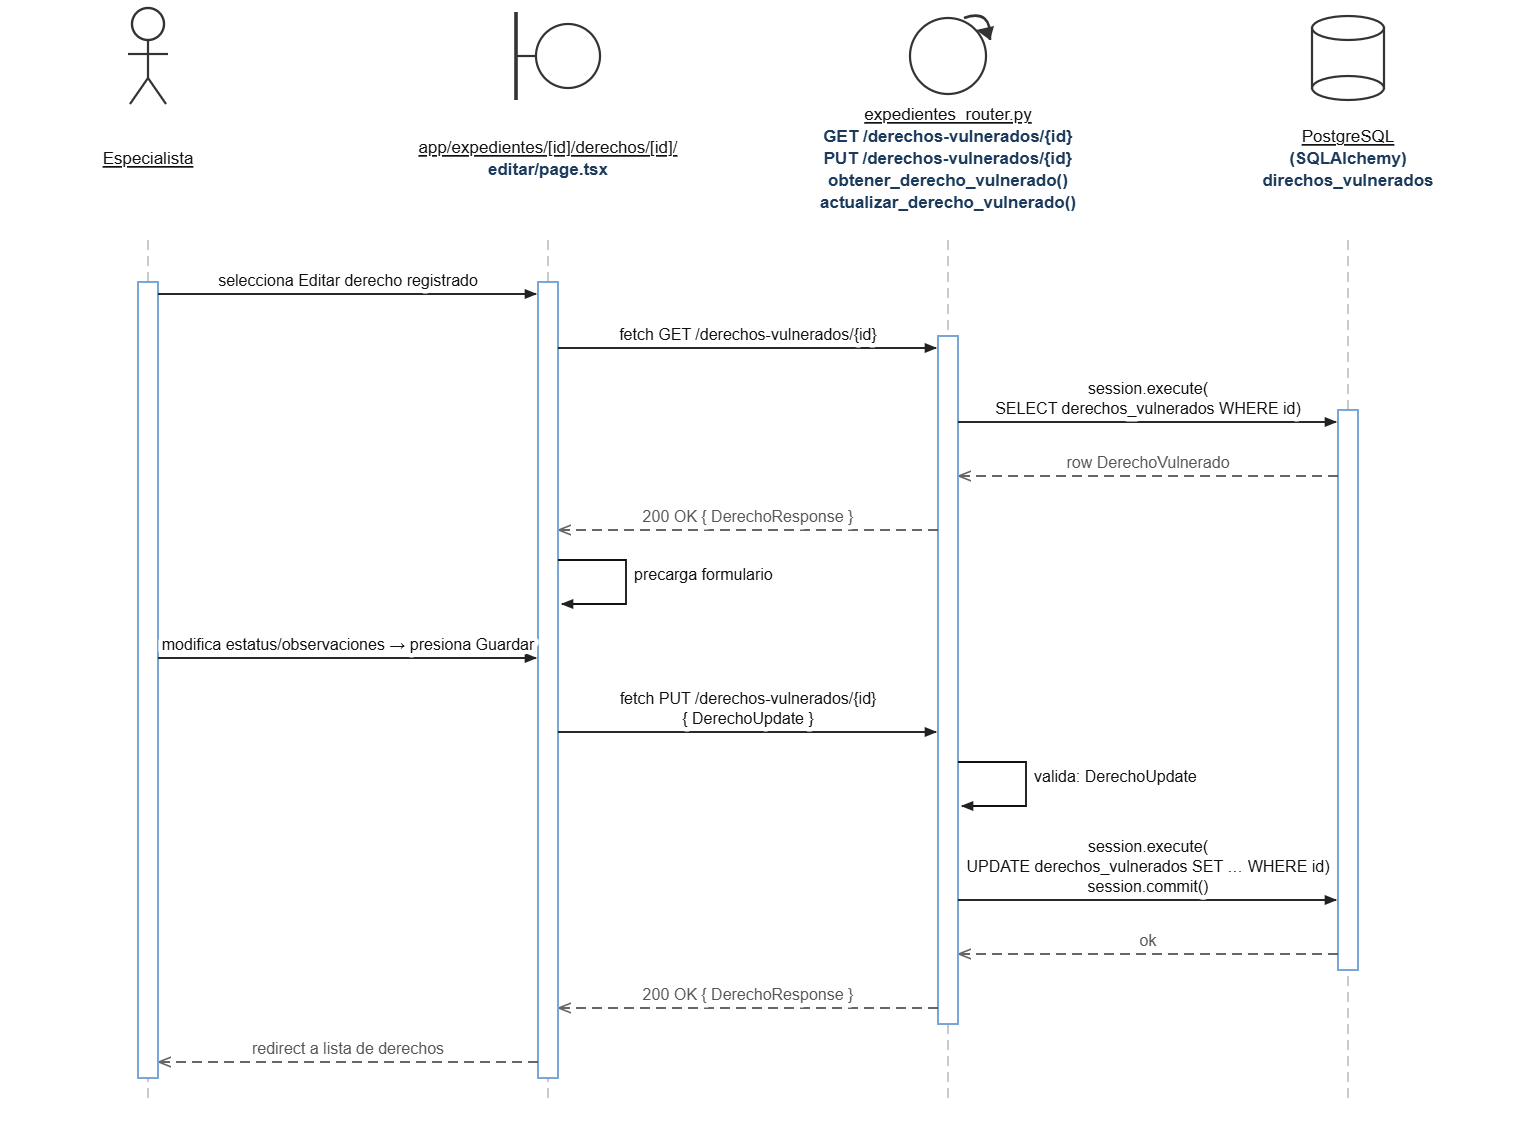
\includegraphics[width=0.8\textwidth]{img/CU-25.png}
	\caption{Diagrama de secuencia --- CU-25 Modificar derecho vulnerado.}
	\label{fig:secuencia-cu25}
\end{figure}

\subsection*{Flujo Alternativo / Excepciones}
\begin{itemize}
	\item \textbf{E1: Registro no encontrado} - Si el identificador del derecho vulnerado no corresponde a ningún registro activo en la base de datos, el sistema aborta y muestra un aviso de error.
	\item \textbf{E2: Falta de justificación de la restitución} - Si se cambia el estado a "Restituido" pero se omiten las observaciones de las medidas tomadas. El sistema deniega el guardado y exige ingresar la justificación.
\end{itemize}

\bigskip
\noindent\rule{\linewidth}{0.5pt}
\bigskip

% ============================================================
\section{Diseño Dinámico del CU: Registrar actor en materia de derechos (CU-26)}
% ============================================================

\subsection*{Descripción del Flujo}
El Especialista accede al directorio e inicia el registro de una institución u organismo externo de apoyo. Completa el formulario con la denominación social, tipo de apoyo (albergue, salud, educación), RFC y datos de contacto de la entidad. Al presionar "Guardar", la interfaz envía los datos al Backend. El Backend verifica en la base de datos que el nombre de la institución y el RFC no estén duplicados. Si son únicos, almacena el nuevo actor en la base de datos con estado "Activo" y responde éxito a la interfaz, que actualiza el directorio.

\begin{figure}[H]
	\centering
	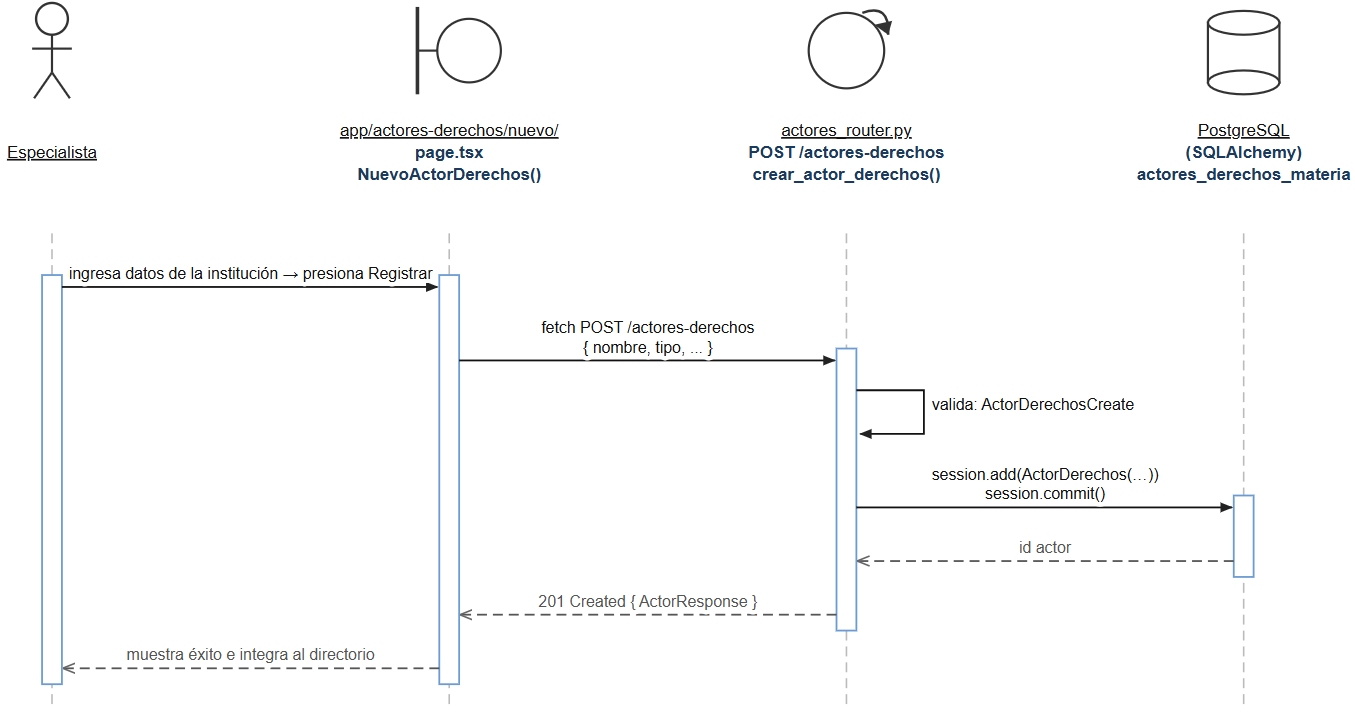
\includegraphics[width=0.8\textwidth]{img/CU26.png}
	\caption{Diagrama de secuencia --- CU-26 Registrar actor en materia de derechos.}
	\label{fig:secuencia-cu26}
\end{figure}

\subsection*{Flujo Alternativo / Excepciones}
\begin{itemize}
	\item \textbf{E1: Nombre de la institución ya registrado} - Ya existe un actor registrado con la misma denominación social. El sistema muestra la advertencia "El nombre de la institución ya existe" y detiene el registro.
	\item \textbf{E2: RFC duplicado} - El RFC ingresado ya pertenece a otra organización en la base de datos. Se bloquea la creación y se regresa al formulario.
\end{itemize}

\bigskip
\noindent\rule{\linewidth}{0.5pt}
\bigskip

% ============================================================
\section{Diseño Dinámico del CU: Consultar actor en materia de derechos (CU-27)}
% ============================================================

\subsection*{Descripción del Flujo}
El Especialista ingresa a la búsqueda del directorio de instituciones aliadas. Selecciona un actor de la lista y la interfaz envía la solicitud de detalles al Backend. El Backend realiza una consulta en la base de datos recopilando la información legal, convenios activos, servicios que ofrece y datos de sus representantes. La base de datos devuelve la información. El Backend la transmite a la interfaz, que despliega de forma completa el perfil del actor en la pantalla.

\begin{figure}[H]
	\centering
	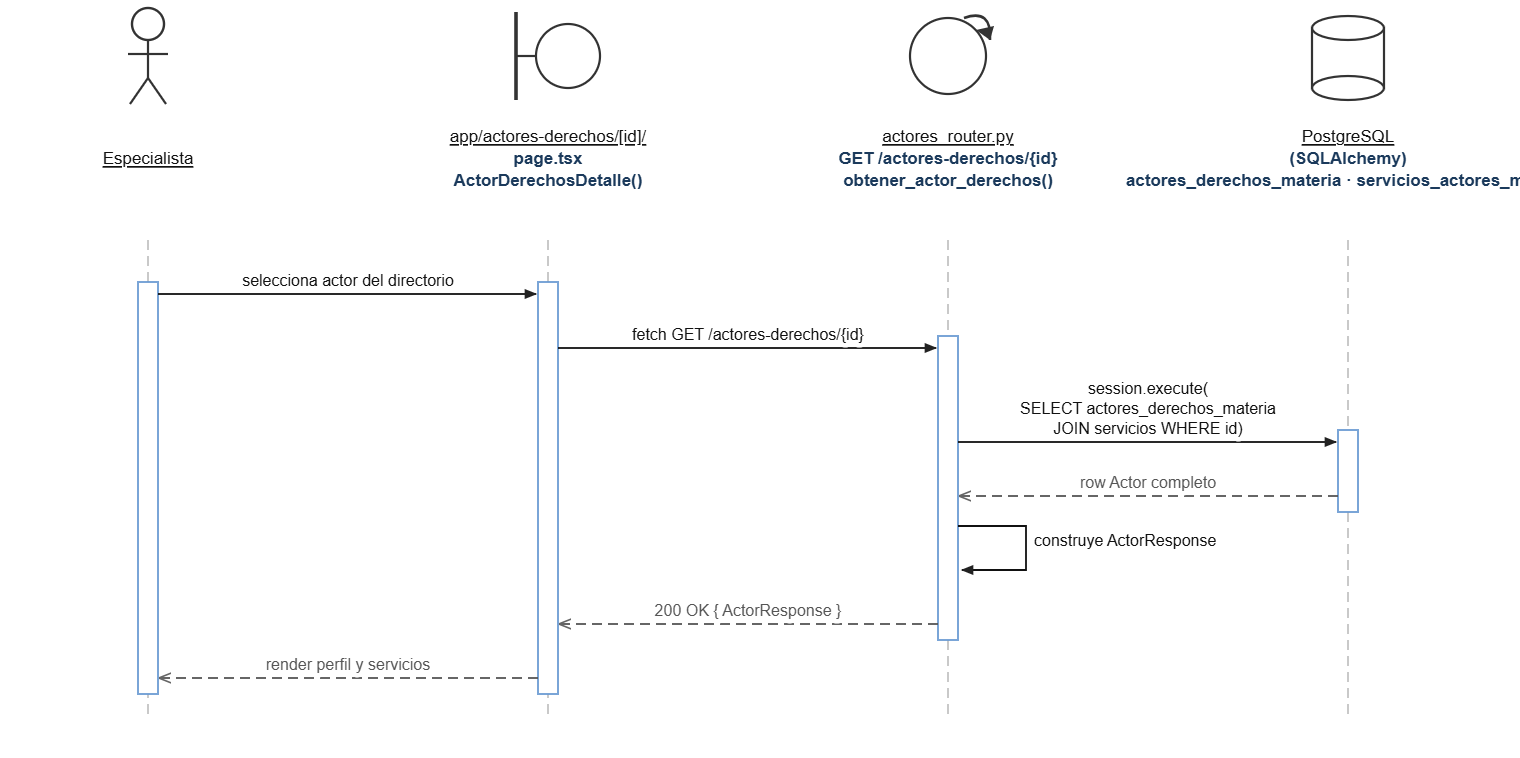
\includegraphics[width=0.8\textwidth]{img/CU-27.png}
	\caption{Diagrama de secuencia --- CU-27 Consultar actor en materia de derechos.}
	\label{fig:secuencia-cu27}
\end{figure}

\subsection*{Flujo Alternativo / Excepciones}
\begin{itemize}
	\item \textbf{E1: Actor no encontrado} - El identificador del actor consultado no corresponde a ningún registro activo en el sistema. Se notifica del error y se regresa al listado general.
\end{itemize}

\bigskip
\noindent\rule{\linewidth}{0.5pt}
\bigskip

% ============================================================
\section{Diseño Dinámico del CU: Modificar actor en materia de derechos (CU-28)}
% ============================================================

\subsection*{Descripción del Flujo}
El Especialista selecciona un actor del directorio y pulsa "Editar". La interfaz presenta el formulario con los campos llenos con la información actual del actor. El Especialista modifica los datos (dirección, tipo de apoyo, teléfono) y presiona "Guardar". El Backend valida que la denominación social modificada no pertenezca a otra institución diferente y que los campos requeridos sigan provistos. Al confirmarse, actualiza el registro en la base de datos y responde con éxito. La interfaz muestra un aviso de guardado exitoso.

\begin{figure}[H]
	\centering
	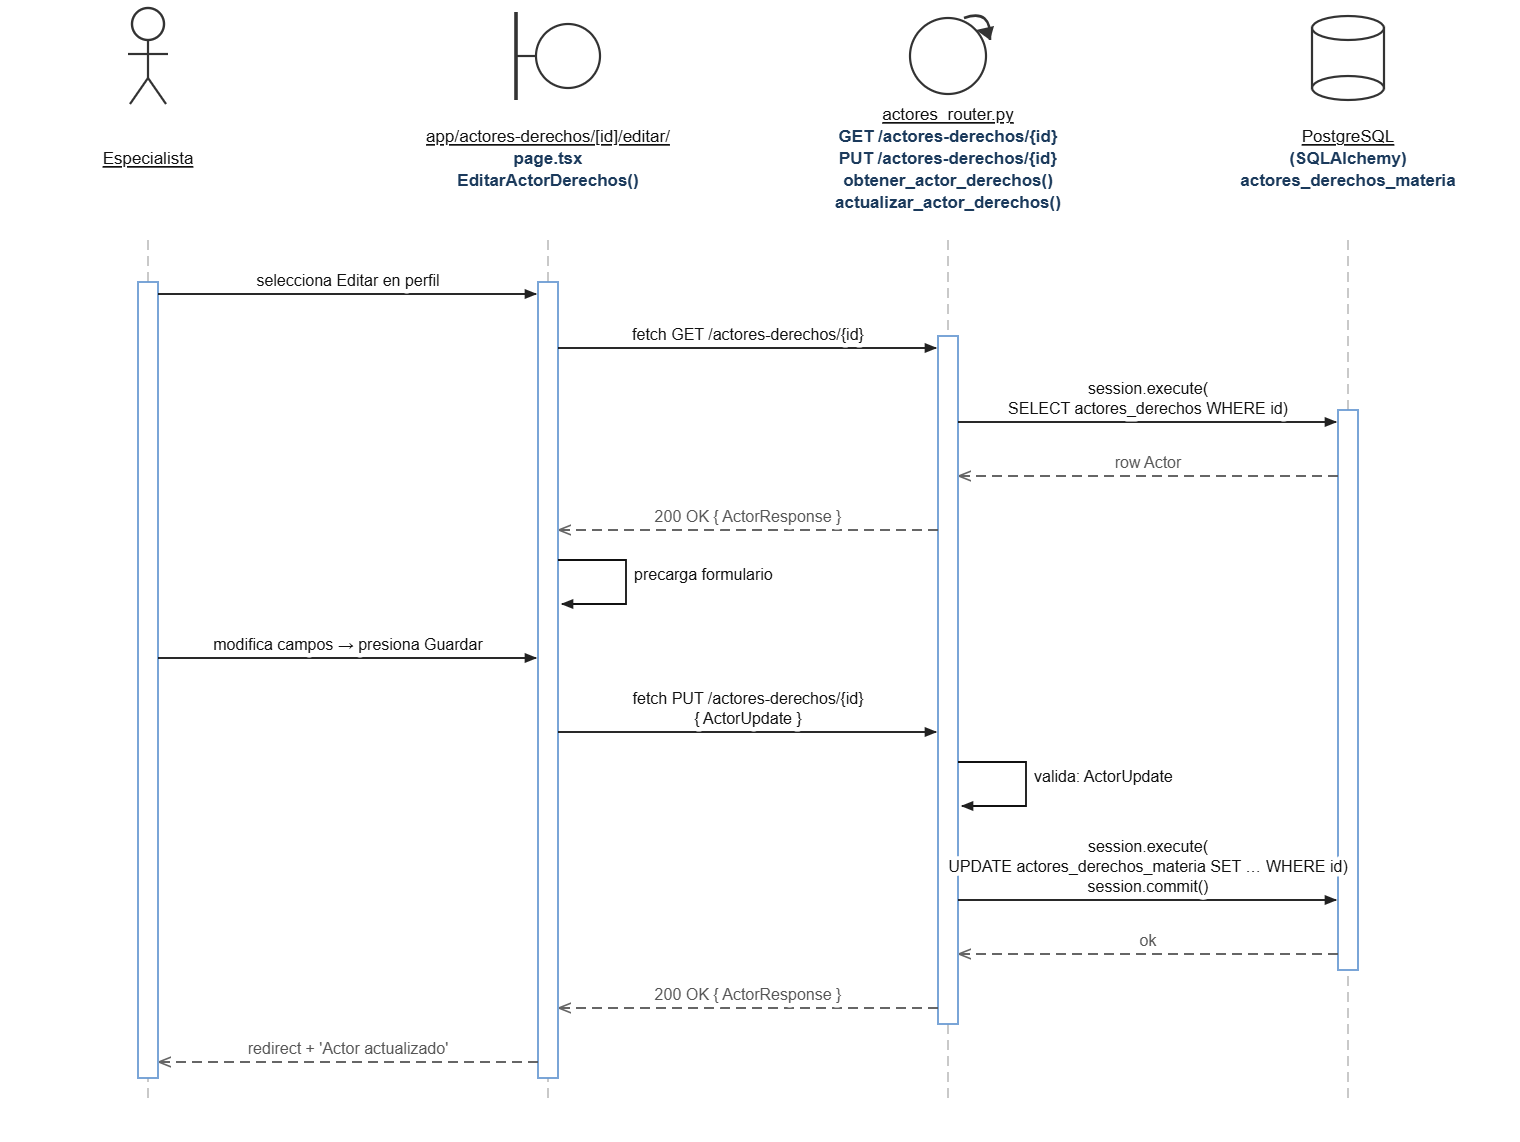
\includegraphics[width=0.8\textwidth]{img/CU-28.png}
	\caption{Diagrama de secuencia --- CU-28 Modificar actor en materia de derechos.}
	\label{fig:secuencia-cu28}
\end{figure}

\subsection*{Flujo Alternativo / Excepciones}
\begin{itemize}
	\item \textbf{E1: Nombre duplicado con otra entidad} - El nombre modificado ya se encuentra en uso por otra institución en la base de datos. El sistema bloquea el cambio y alerta de la colisión.
	\item \textbf{E2: Campos obligatorios vacíos} - Si se omiten datos indispensables en el formulario de edición, la interfaz cancela el guardado.
\end{itemize}

\bigskip
\noindent\rule{\linewidth}{0.5pt}
\bigskip

% ============================================================
\section{Diseño Dinámico del CU: Eliminar actor en materia de derechos (CU-29)}
% ============================================================

\subsection*{Descripción del Flujo}
El Especialista selecciona un actor en el directorio y hace clic en "Eliminar". La interfaz muestra un cuadro de diálogo solicitando la confirmación de la eliminación física. Al confirmar, se envía la solicitud al Backend. El Backend comprueba en la base de datos si la institución tiene convenios, canalizaciones o programas asociados a expedientes activos de NNA. Si está libre de dependencias, elimina el registro de la base de datos y devuelve éxito. La interfaz actualiza el listado del directorio.

\begin{figure}[H]
	\centering
	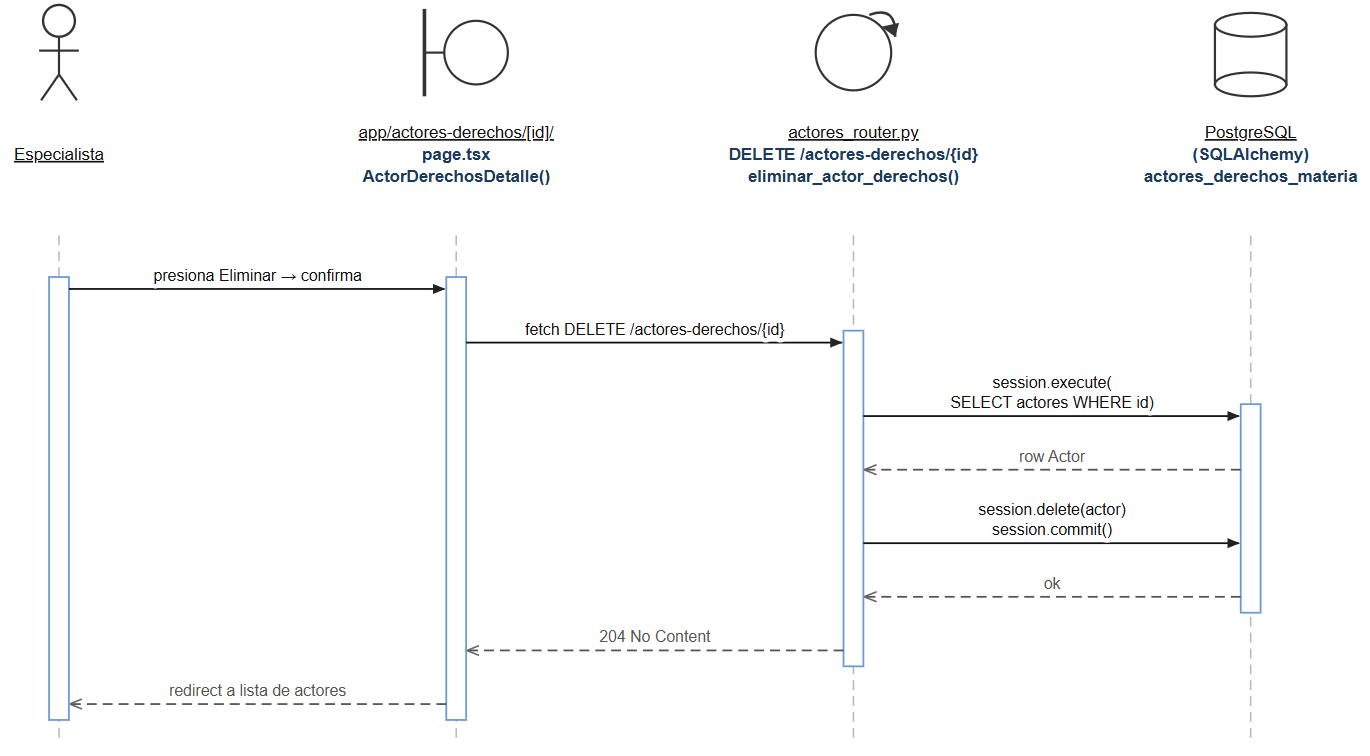
\includegraphics[width=0.8\textwidth]{img/CU29.png}
	\caption{Diagrama de secuencia --- CU-29 Eliminar actor en materia de derechos.}
	\label{fig:secuencia-cu29}
\end{figure}

\subsection*{Flujo Alternativo / Excepciones}
\begin{itemize}
	\item \textbf{E1: Actor con dependencias activas} - El actor tiene programas o canalizaciones de menores asociadas. El Backend rechaza la eliminación y devuelve un error. La interfaz muestra un mensaje sugiriendo deshabilitar al actor en lugar de eliminarlo.
	\item \textbf{E2: Cancelación de la eliminación} - El usuario cancela la confirmación en el modal. La interfaz cierra la ventana y el actor no sufre modificaciones.
\end{itemize}

\bigskip
\noindent\rule{\linewidth}{0.5pt}
\bigskip

% ============================================================
\section{Diseño Dinámico del CU: Registrar servicio de actor (CU-30)}
% ============================================================

\subsection*{Descripción del Flujo}
El Especialista ingresa al perfil de un actor institucional y selecciona "Añadir servicio de apoyo". Completa los datos del servicio (nombre, descripción, categoría, requisitos, costo o gratuidad) y presiona "Guardar". La interfaz envía el ID del actor y los datos del servicio al Backend. El Backend valida que el actor exista y esté activo en la base de datos, y guarda el nuevo servicio de apoyo vinculado al actor en la base de datos. El Backend confirma el registro del servicio y la interfaz refresca el perfil del actor.

\begin{figure}[H]
	\centering
	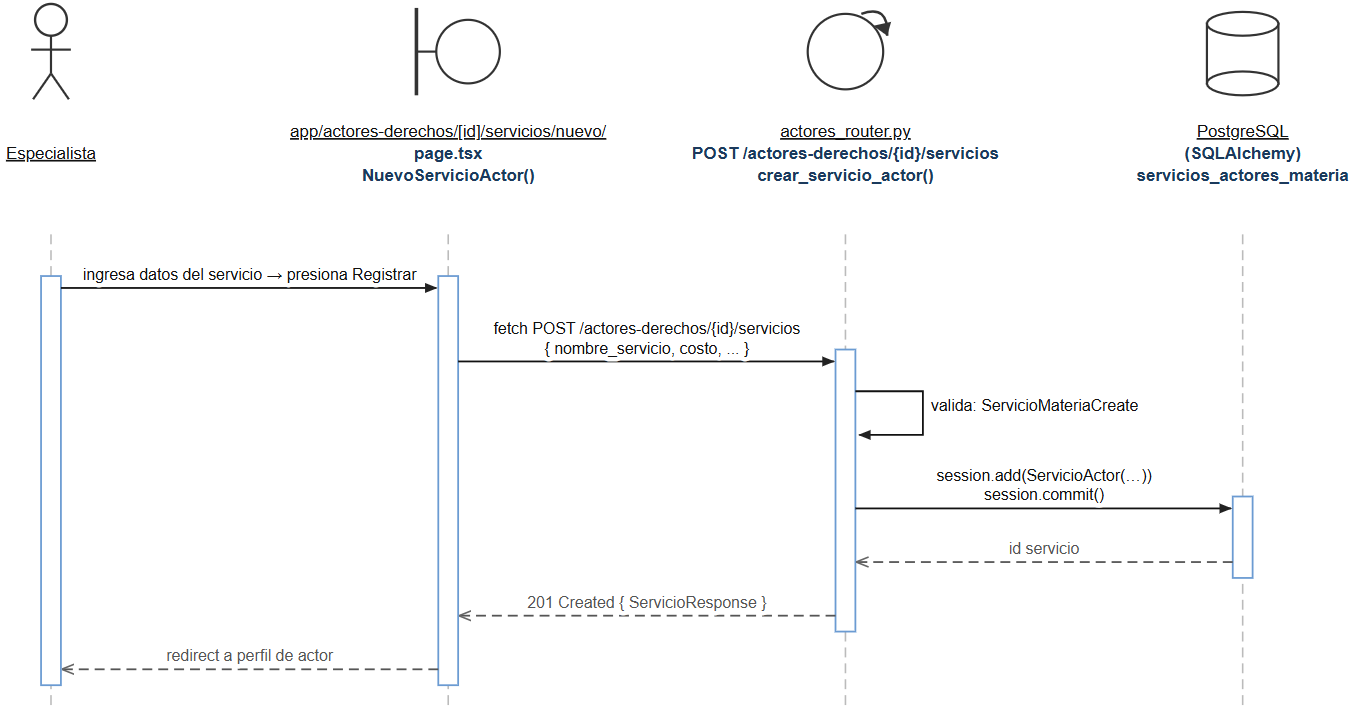
\includegraphics[width=0.8\textwidth]{img/CU30.png}
	\caption{Diagrama de secuencia --- CU-30 Registrar servicio de actor.}
	\label{fig:secuencia-cu30}
\end{figure}

\subsection*{Flujo Alternativo / Excepciones}
\begin{itemize}
	\item \textbf{E1: Costo del servicio inválido} - Si el servicio es de pago pero se ingresa un costo no numérico o negativo. El sistema detiene el proceso y marca el campo del costo.
	\item \textbf{E2: Actor asociado inactivo} - El actor al que se intenta agregar el servicio está deshabilitado en la base de datos. El Backend deniega la operación.
\end{itemize}

\bigskip
\noindent\rule{\linewidth}{0.5pt}
\bigskip

% ============================================================
\section{Diseño Dinámico del CU: Consultar actores por municipio y tipo de servicio (CU-31)}
% ============================================================

\subsection*{Descripción del Flujo}
El Especialista busca alternativas de vinculación para un caso. Introduce el municipio y el tipo de servicio requerido (ejemplo: albergue) en el motor de búsqueda de canalizaciones. La interfaz envía los filtros de búsqueda al Backend. El Backend ejecuta una consulta select con filtros JOIN sobre las tablas de actores, ubicaciones y servicios en la base de datos. La base de datos devuelve la lista de instituciones coincidentes. El Backend envía el listado a la interfaz de usuario, la cual presenta en pantalla las opciones con su información de contacto.

\begin{figure}[H]
	\centering
	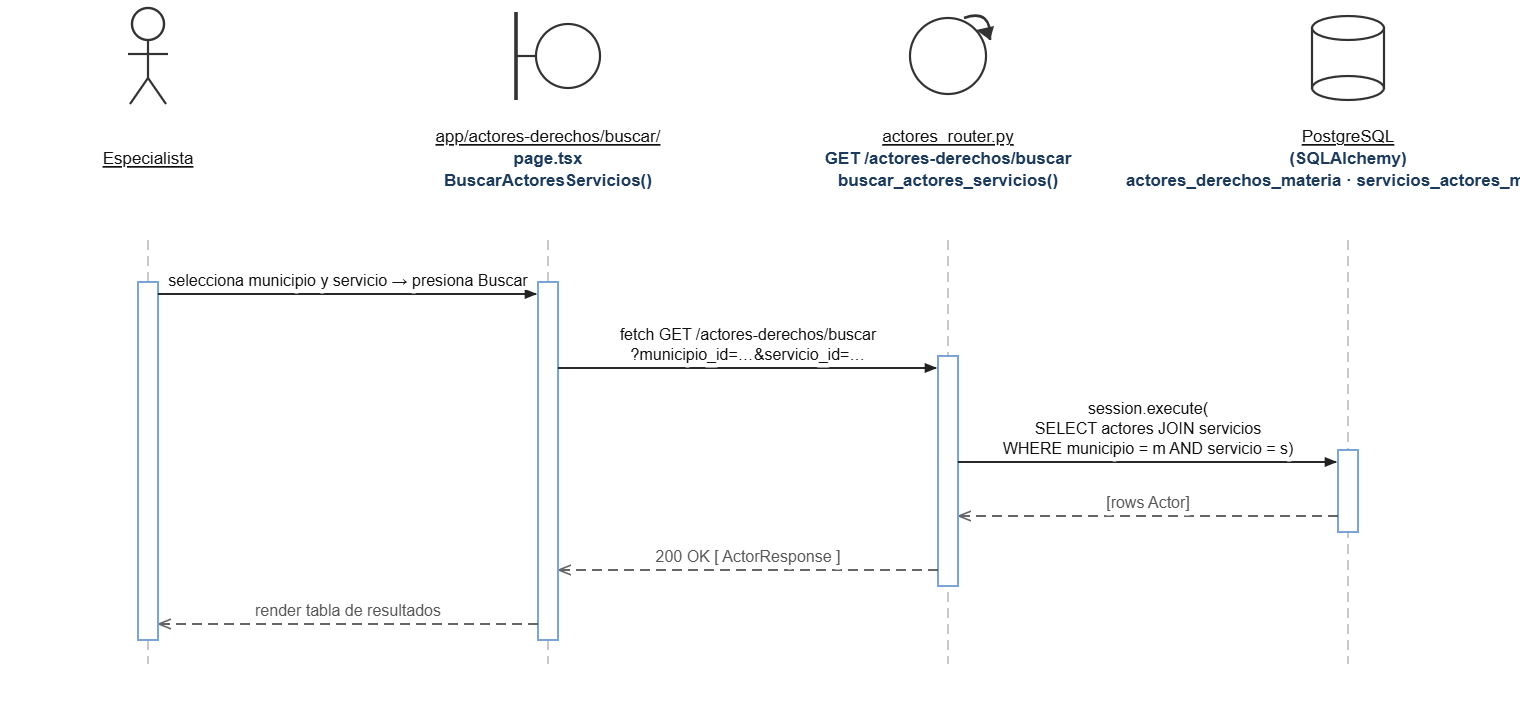
\includegraphics[width=0.8\textwidth]{img/CU-31.png}
	\caption{Diagrama de secuencia --- CU-31 Consultar actores por municipio y tipo de servicio.}
	\label{fig:secuencia-cu31}
\end{figure}

\subsection*{Flujo Alternativo / Excepciones}
\begin{itemize}
	\item \textbf{E1: Sin resultados coincidentes} - Ninguna institución ofrece ese servicio en el municipio seleccionado. El sistema notifica al usuario indicando que no se encontraron coincidencias para los criterios indicados y sugiere ampliar la búsqueda.
\end{itemize}

\bigskip
\noindent\rule{\linewidth}{0.5pt}
\bigskip

% ============================================================
\section{Diseño Dinámico del CU: Consultar catálogo de domicilios (SEPOMEX) (CU-32)}
% ============================================================

\subsection*{Descripción del Flujo}
Durante la captura de cualquier dirección en los formularios del sistema, el usuario digita un Código Postal de 5 dígitos. Al completarse los dígitos, la interfaz envía una petición automática GET al Backend con el CP. El Backend realiza una búsqueda indexada en la tabla de catálogo SEPOMEX de la base de datos. La base de datos devuelve el estado, el municipio y el listado de asentamientos (colonias) correspondientes al CP. El Backend responde con estos datos y la interfaz autocompleta los campos de Estado y Municipio y carga las opciones de Colonias en un menú desplegable para que el usuario elija una de ellas.

\begin{figure}[H]
	\centering
	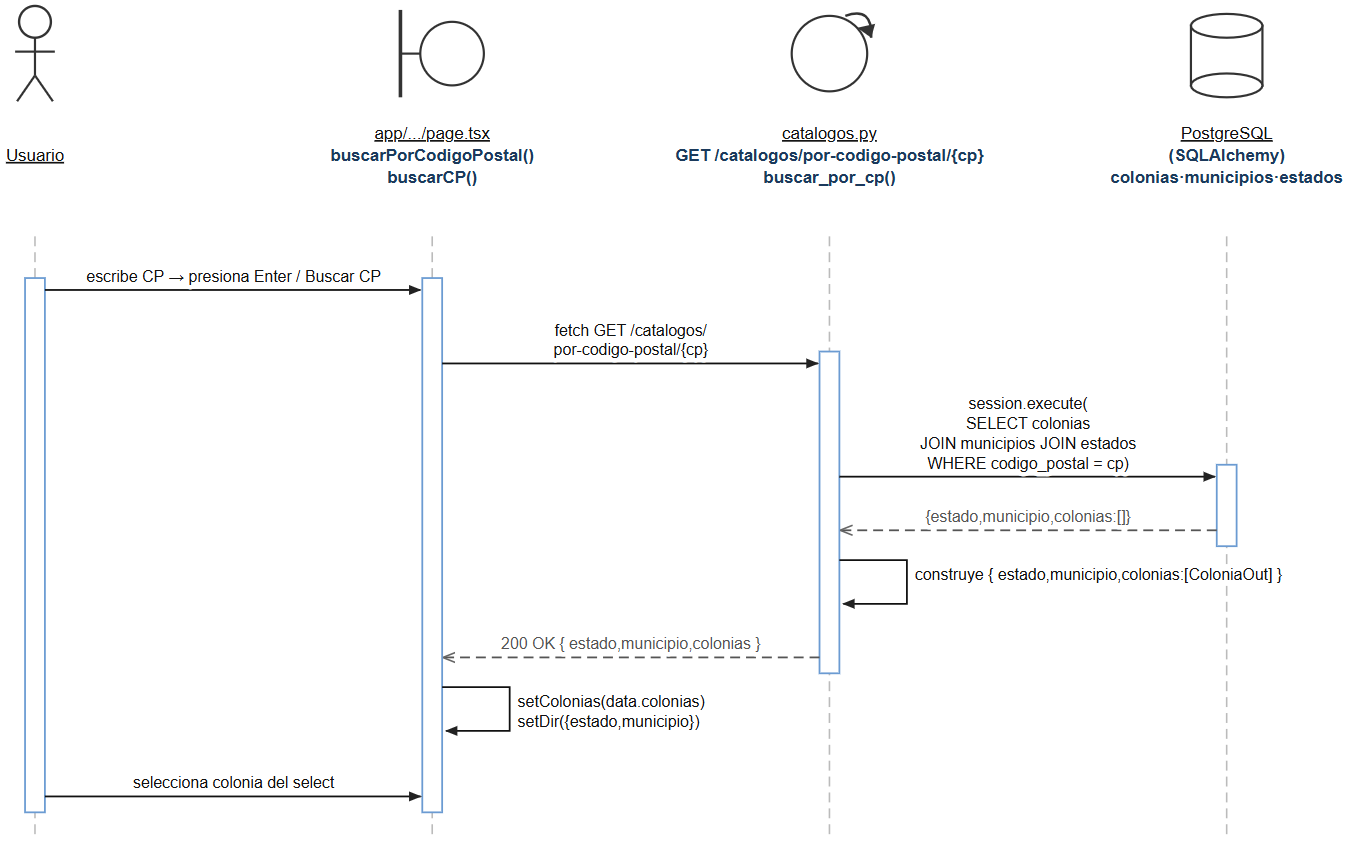
\includegraphics[width=0.8\textwidth]{img/CU32.png}
	\caption{Diagrama de secuencia --- CU-32 Consultar catálogo de domicilios (SEPOMEX).}
	\label{fig:secuencia-cu32}
\end{figure}

\subsection*{Flujo Alternativo / Excepciones}
\begin{itemize}
	\item \textbf{E1: Código Postal no encontrado} - El CP ingresado no existe en el catálogo cargado en la base de datos. El sistema muestra la advertencia "Código postal no encontrado" y habilita la captura manual libre de todos los campos de dirección.
\end{itemize}

\bigskip
\noindent\rule{\linewidth}{0.5pt}
\bigskip

% ============================================================
\section{Diseño Dinámico del CU: Consultar catálogo de idiomas (INALI) (CU-33)}
% ============================================================

\subsection*{Descripción del Flujo}
Al registrar o modificar a un NNA o tutor, el Especialista hace clic en la sección de Lengua / Idioma. La interfaz solicita el listado al Backend. El Backend realiza una consulta a la tabla del catálogo INALI en la base de datos para extraer los idiomas y variantes lingüísticas registradas. La base de datos devuelve el listado. El Backend envía los datos a la interfaz, que despliega un componente de autocompletado y selección múltiple en pantalla para facilitar la elección homogénea del idioma del menor.

\begin{figure}[H]
	\centering
	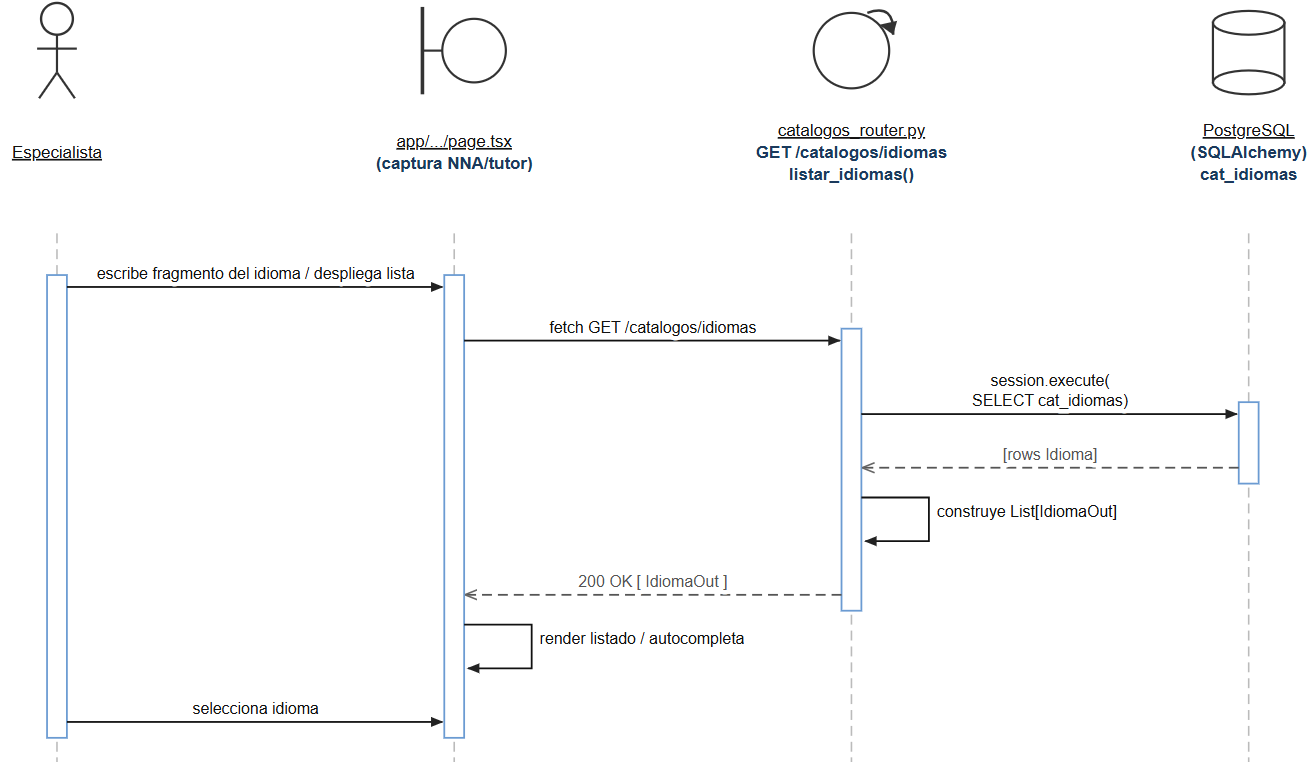
\includegraphics[width=0.8\textwidth]{img/CU33.png}
	\caption{Diagrama de secuencia --- CU-33 Consultar catálogo de idiomas (INALI).}
	\label{fig:secuencia-cu33}
\end{figure}

\subsection*{Flujo Alternativo / Excepciones}
\begin{itemize}
	\item \textbf{E1: Fallo de carga del catálogo} - Si no se pueden obtener los datos del catálogo por un error en el servidor, el sistema habilita temporalmente un campo de texto libre para que el Especialista ingrese el idioma manualmente.
\end{itemize}

\bigskip
\noindent\rule{\linewidth}{0.5pt}
\bigskip

% ============================================================
\section{Diseño Dinámico del CU: Registrar discapacidad de NNA o tutor (CU-34)}
% ============================================================

\subsection*{Descripción del Flujo}
El Especialista ingresa al expediente clínico del NNA o del tutor. Selecciona "Añadir discapacidad". La interfaz despliega la lista oficial de discapacidades registradas en el sistema. El Especialista selecciona el tipo de discapacidad e introduce observaciones específicas sobre la condición física o psíquica y presiona "Guardar". El Backend verifica que el paciente no tenga ya asociada la misma discapacidad en la base de datos y registra la discapacidad en la base de datos. Finalmente, devuelve el éxito de la inserción y la interfaz actualiza la vista de salud.

\begin{figure}[H]
	\centering
	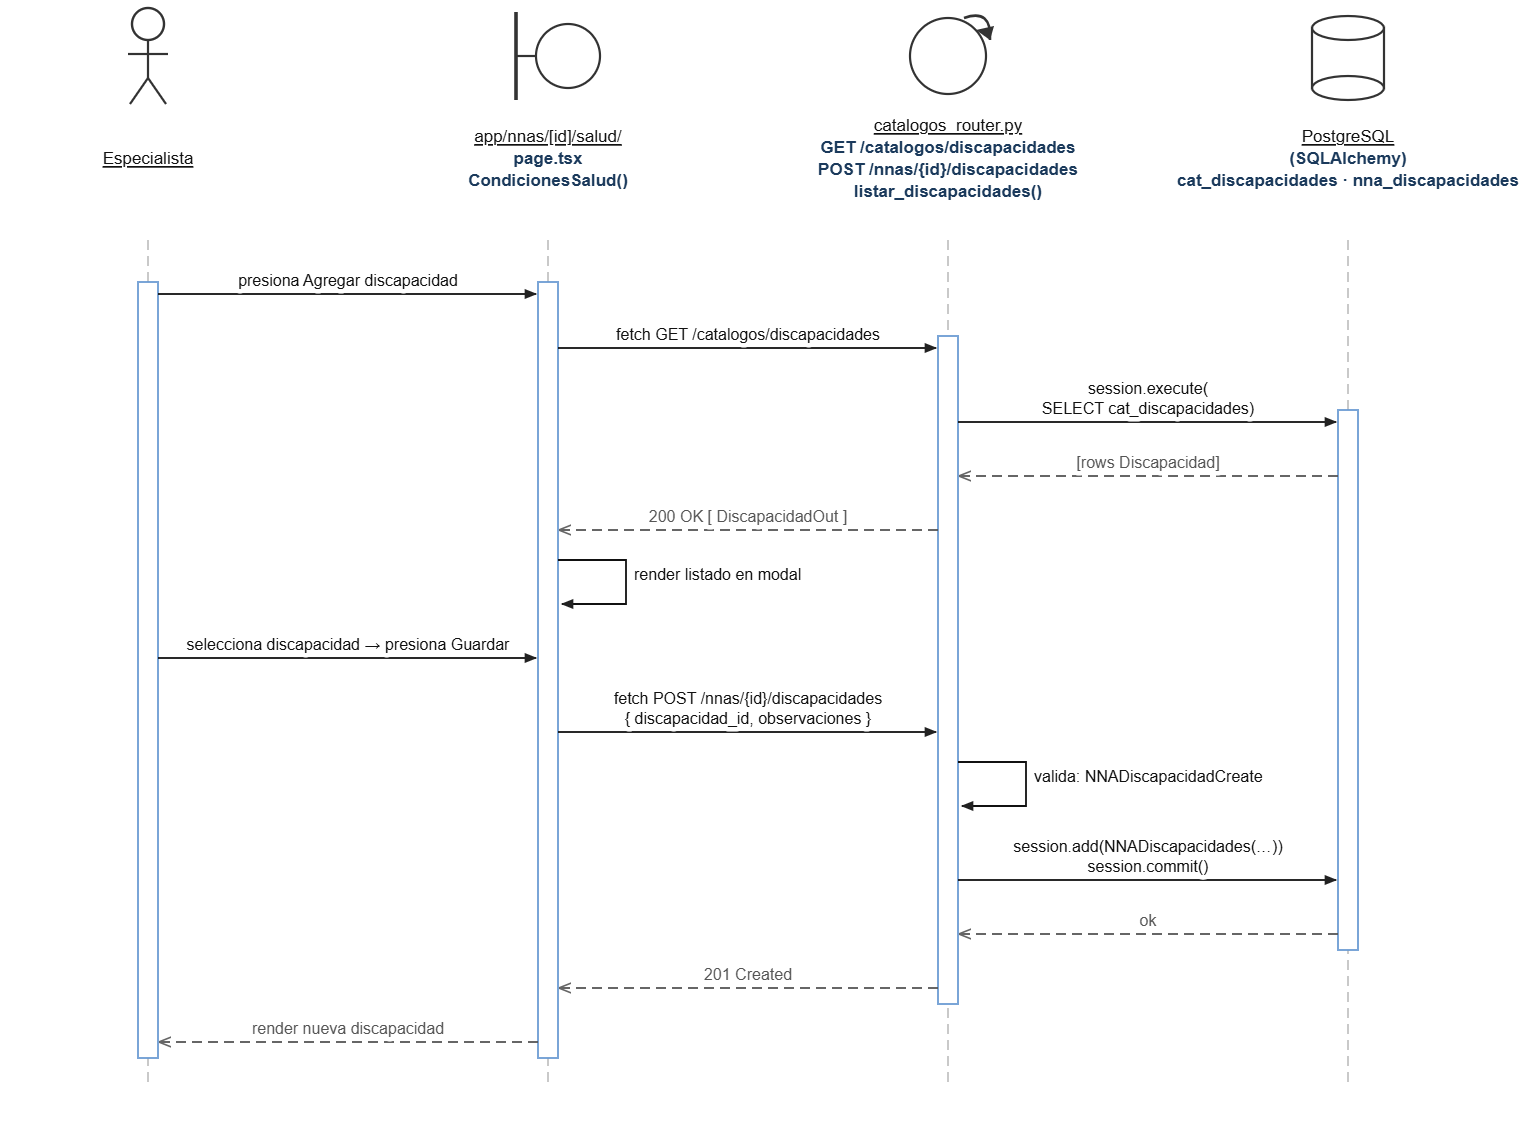
\includegraphics[width=0.8\textwidth]{img/CU-34.png}
	\caption{Diagrama de secuencia --- CU-34 Registrar discapacidad de NNA o tutor.}
	\label{fig:secuencia-cu34}
\end{figure}

\subsection*{Flujo Alternativo / Excepciones}
\begin{itemize}
	\item \textbf{E1: Discapacidad ya registrada} - El menor o tutor ya tiene registrada la misma discapacidad en su perfil. El sistema bloquea el duplicado y muestra "La discapacidad ya se encuentra registrada".
	\item \textbf{E2: No se seleccionó tipo de discapacidad} - El Especialista intenta guardar sin elegir una opción de la lista. El sistema detiene la acción y solicita seleccionar una.
\end{itemize}

\bigskip
\noindent\rule{\linewidth}{0.5pt}
\bigskip

% ============================================================
\section{Diseño Dinámico del CU: Modificar discapacidad de NNA o tutor (CU-35)}
% ============================================================

\subsection*{Descripción del Flujo}
El Especialista localiza una discapacidad en el expediente del NNA o tutor y hace clic en "Editar". La interfaz abre el formulario con el tipo de discapacidad y las observaciones. El Especialista actualiza la descripción o grado de la misma y guarda. El Backend valida que el registro exista en la base de datos y aplica la actualización sobre la tabla de discapacidades asociadas de la base de datos, retornando éxito. La interfaz actualiza el expediente de salud.

\begin{figure}[H]
	\centering
	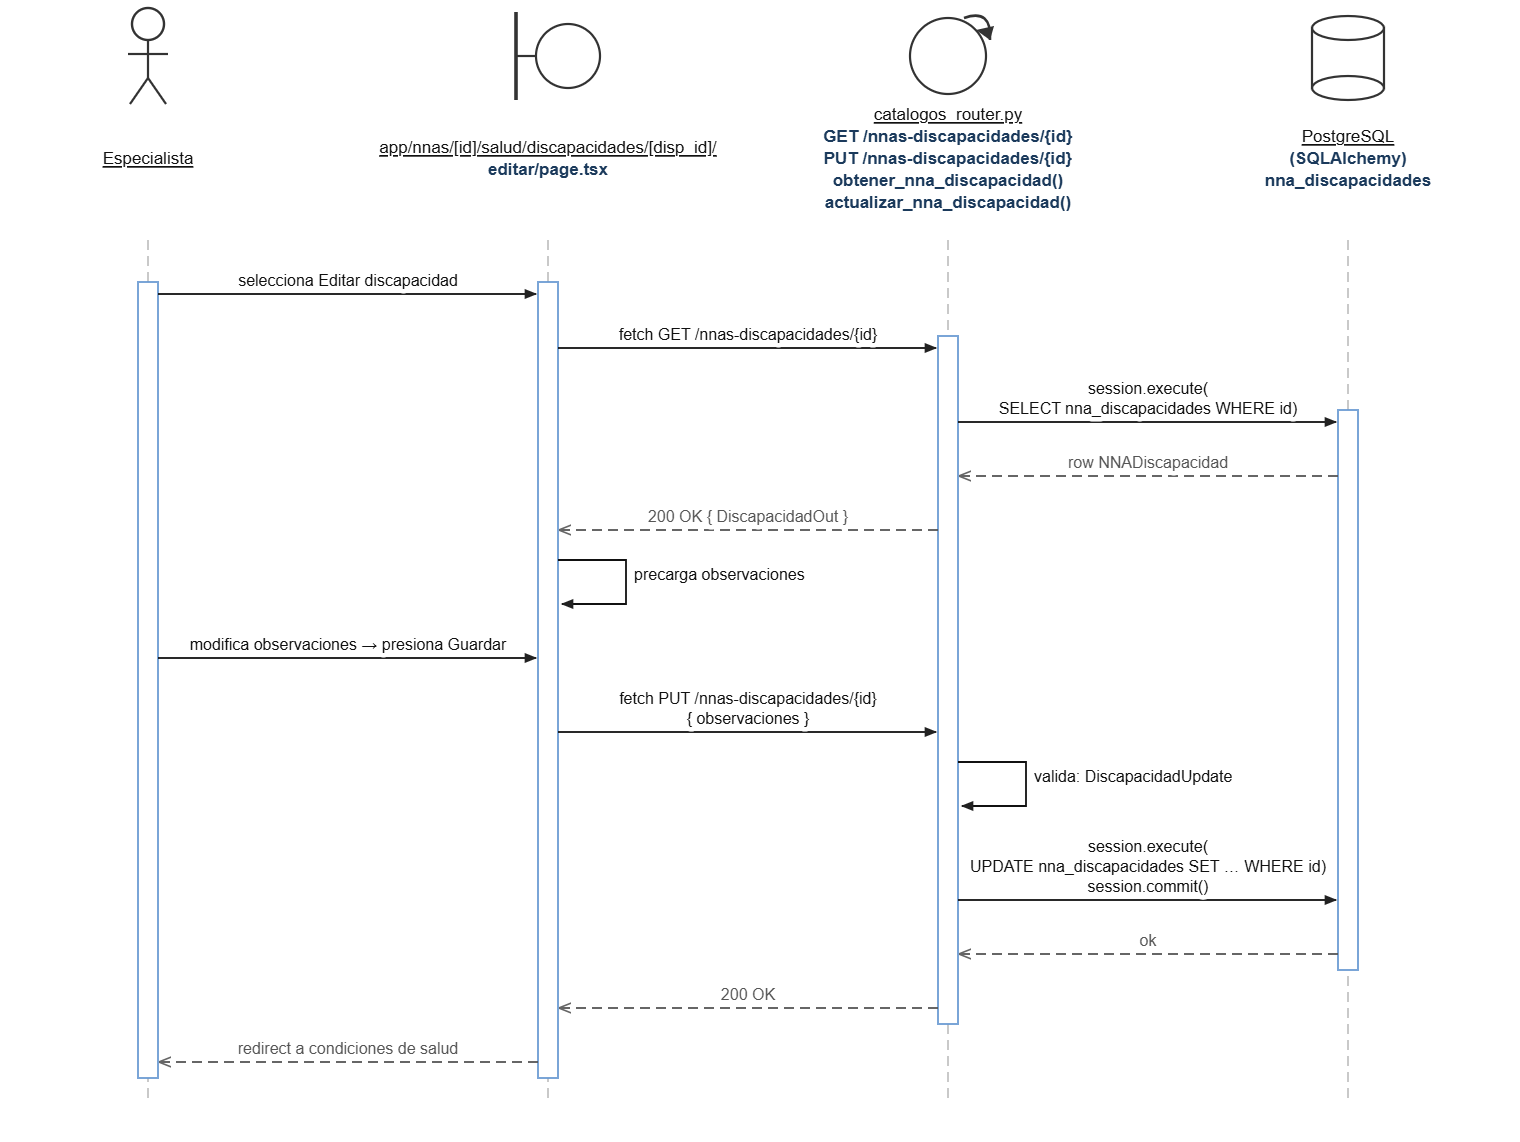
\includegraphics[width=0.8\textwidth]{img/CU-35.png}
	\caption{Diagrama de secuencia --- CU-35 Modificar discapacidad de NNA o tutor.}
	\label{fig:secuencia-cu35}
\end{figure}

\subsection*{Flujo Alternativo / Excepciones}
\begin{itemize}
	\item \textbf{E1: Registro de discapacidad no encontrado} - Si el identificador de la relación no existe, se cancela la operación y se muestra una alerta.
\end{itemize}

\bigskip
\noindent\rule{\linewidth}{0.5pt}
\bigskip

% ============================================================
\section{Diseño Dinámico del CU: Registrar enfermedad de NNA o tutor (CU-36)}
% ============================================================

\subsection*{Descripción del Flujo}
El Especialista ingresa a la ficha de salud del NNA o tutor y pulsa "Añadir enfermedad". Selecciona la enfermedad o padecimiento (ej. diabetes, asma, etc.) de la lista oficial e ingresa observaciones de tratamiento, dosis o cuidados necesarios. Al presionar "Guardar", la interfaz envía los datos al Backend. El Backend comprueba que no esté duplicada la enfermedad activa en el paciente y guarda la enfermedad en la base de datos. El sistema notifica del registro exitoso y actualiza la sección médica.

\begin{figure}[H]
	\centering
	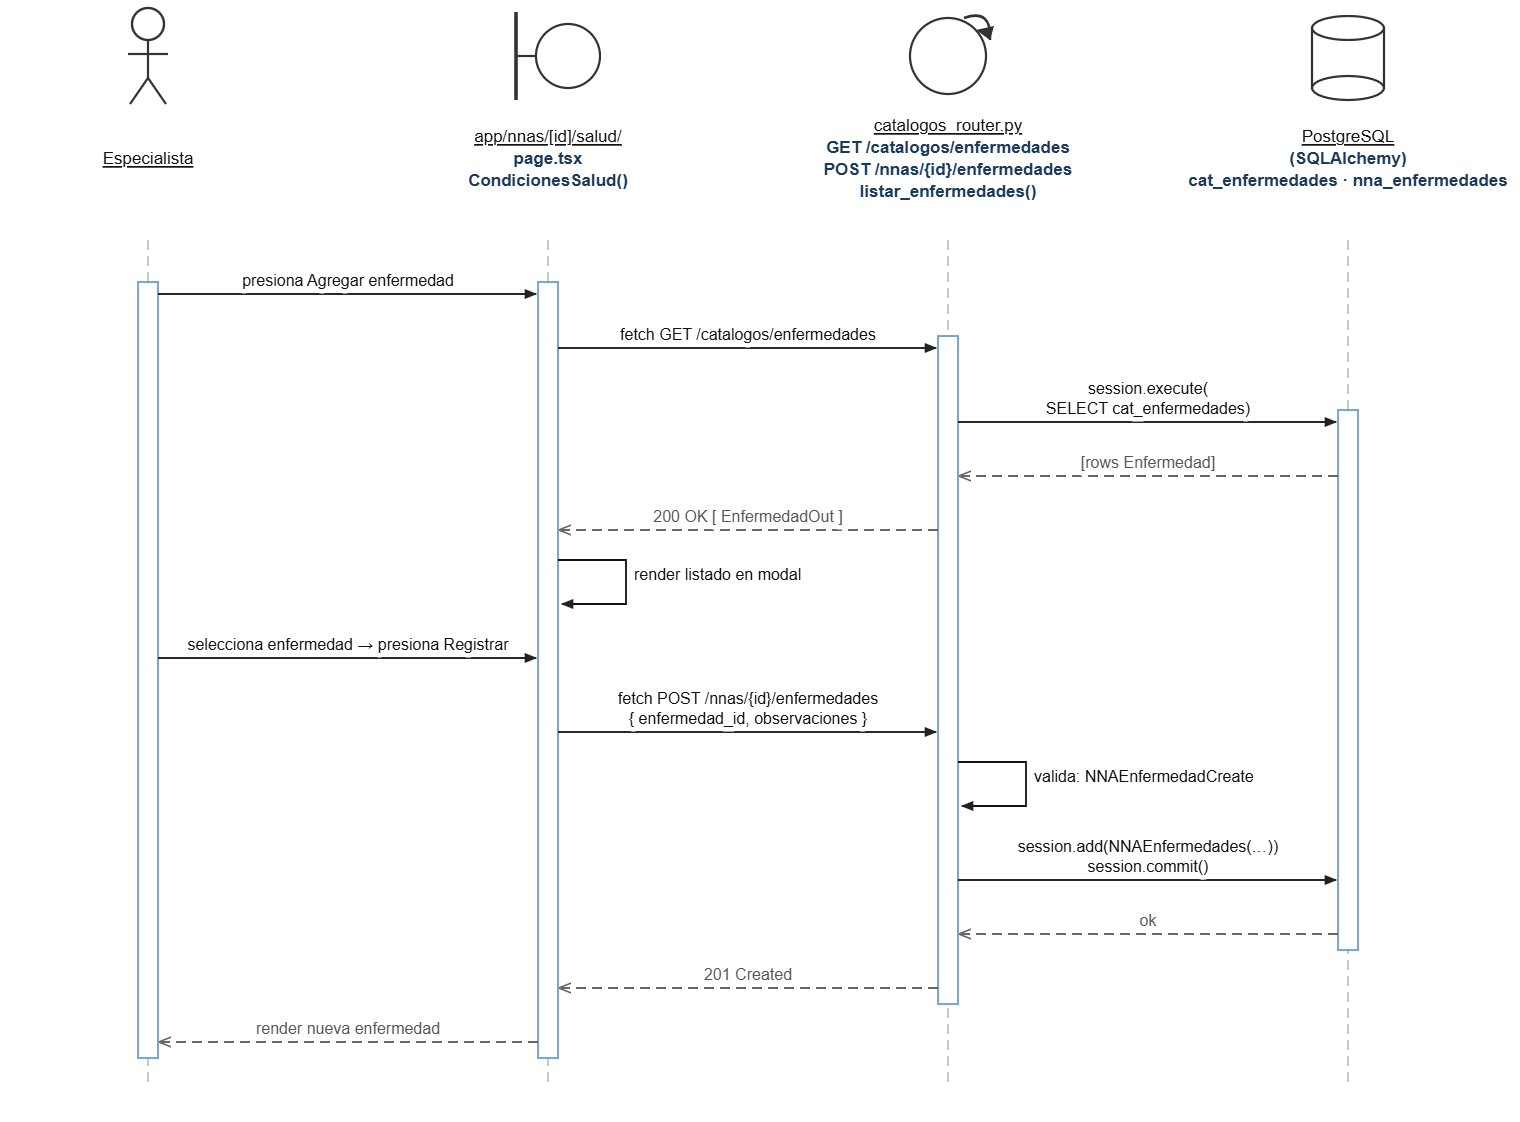
\includegraphics[width=0.8\textwidth]{img/CU-36.png}
	\caption{Diagrama de secuencia --- CU-36 Registrar enfermedad de NNA o tutor.}
	\label{fig:secuencia-cu36}
\end{figure}

\subsection*{Flujo Alternativo / Excepciones}
\begin{itemize}
	\item \textbf{E1: No se especificó la enfermedad} - El Especialista no selecciona ninguna enfermedad de la lista. El sistema detiene el proceso y muestra una alerta solicitando elegir una opción.
	\item \textbf{E2: Enfermedad ya registrada} - El paciente ya cuenta con el registro de esa enfermedad activa en su expediente de salud.
\end{itemize}

\bigskip
\noindent\rule{\linewidth}{0.5pt}
\bigskip

% ============================================================
\section{Diseño Dinámico del CU: Modificar enfermedad de NNA o tutor (CU-37)}
% ============================================================

\subsection*{Descripción del Flujo}
El Especialista localiza el registro de una enfermedad en el perfil del paciente y selecciona "Editar". Modifica el estado de la enfermedad (ejemplo: controlada, inactiva) o actualiza las observaciones de tratamiento y guarda. El Backend valida el registro de la relación, actualiza la información en la base de datos y responde éxito. La interfaz actualiza el estado clínico en pantalla.

\begin{figure}[H]
	\centering
	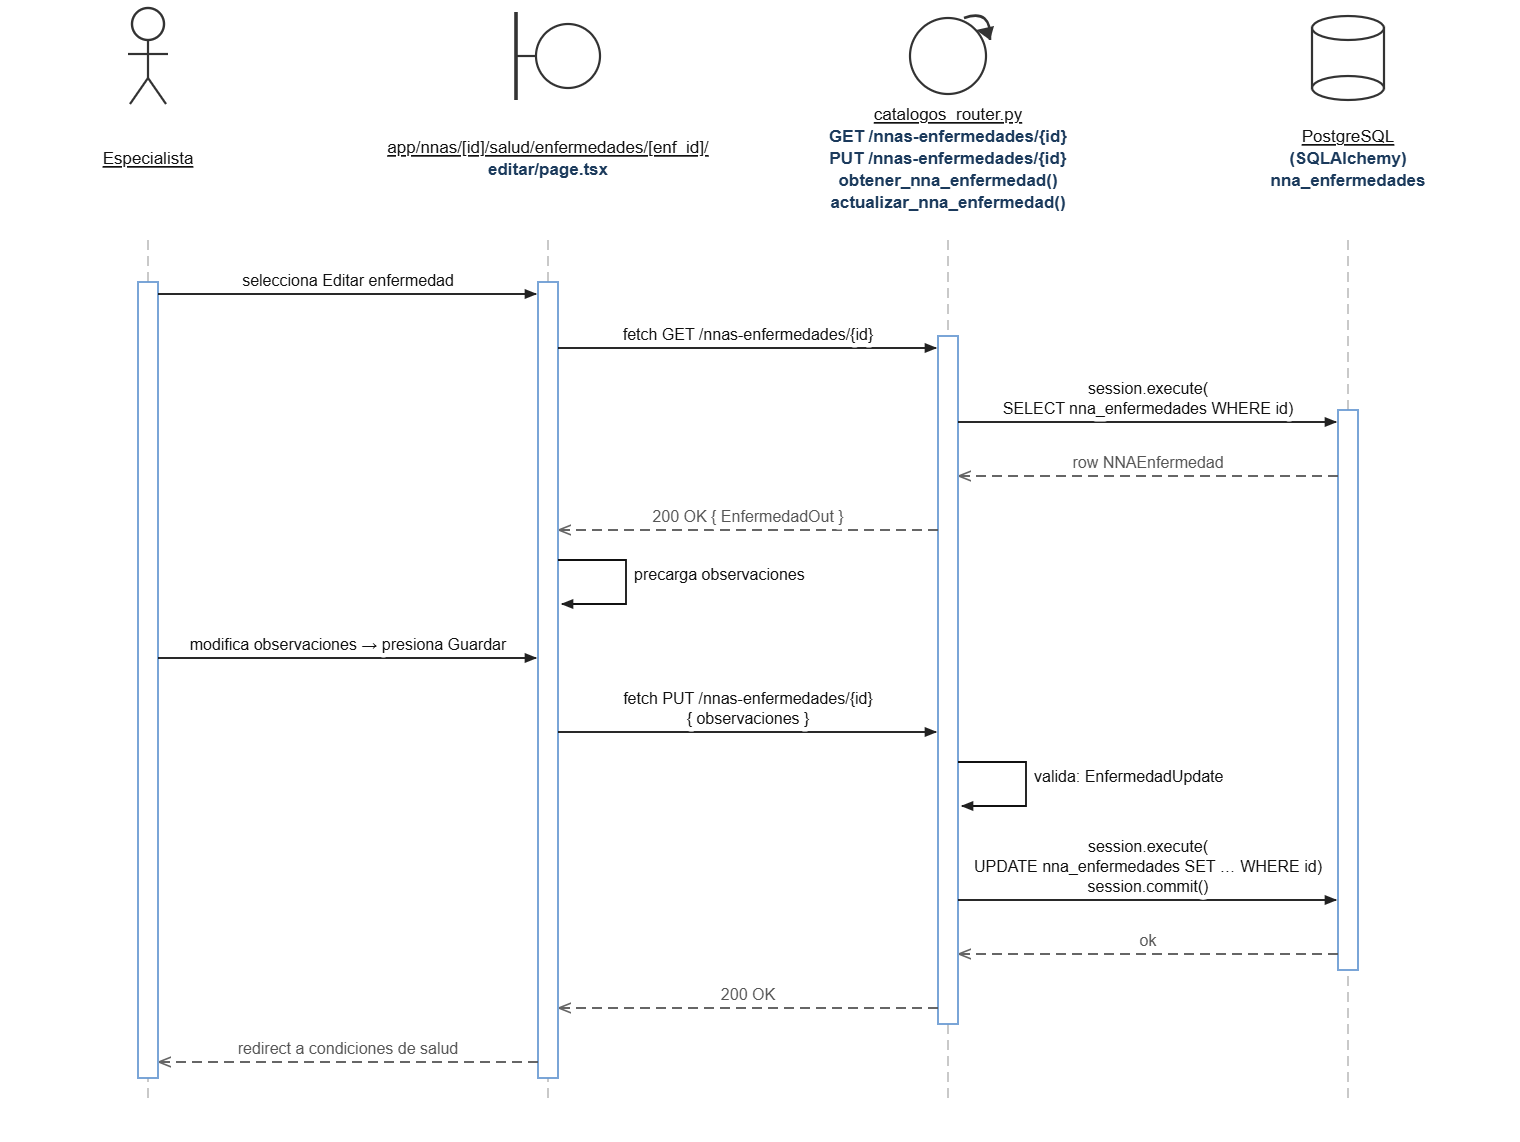
\includegraphics[width=0.8\textwidth]{img/CU-37.png}
	\caption{Diagrama de secuencia --- CU-37 Modificar enfermedad de NNA o tutor.}
	\label{fig:secuencia-cu37}
\end{figure}

\subsection*{Flujo Alternativo / Excepciones}
\begin{itemize}
	\item \textbf{E1: Registro no encontrado} - Si el identificador de la enfermedad asociada no existe en la base de datos.
\end{itemize}

\bigskip
\noindent\rule{\linewidth}{0.5pt}
\bigskip

% ============================================================
\section{Diseño Dinámico del CU: Consultar calendario de expedientes (CU-38)}
% ============================================================

\subsection*{Descripción del Flujo}
El Especialista ingresa al módulo de Calendario de la plataforma. La interfaz solicita las actividades agendadas para el mes actual al Backend. El Backend ejecuta una consulta select filtrando por el rango de fechas mensual y por el ID de los expedientes a los que tiene acceso el Especialista. La base de datos devuelve todos los registros de audiencias, valoraciones y citas. El Backend recopila la lista y la envía a la interfaz, que dibuja los eventos en la cuadrícula del calendario interactivo del Especialista.

\begin{figure}[H]
	\centering
	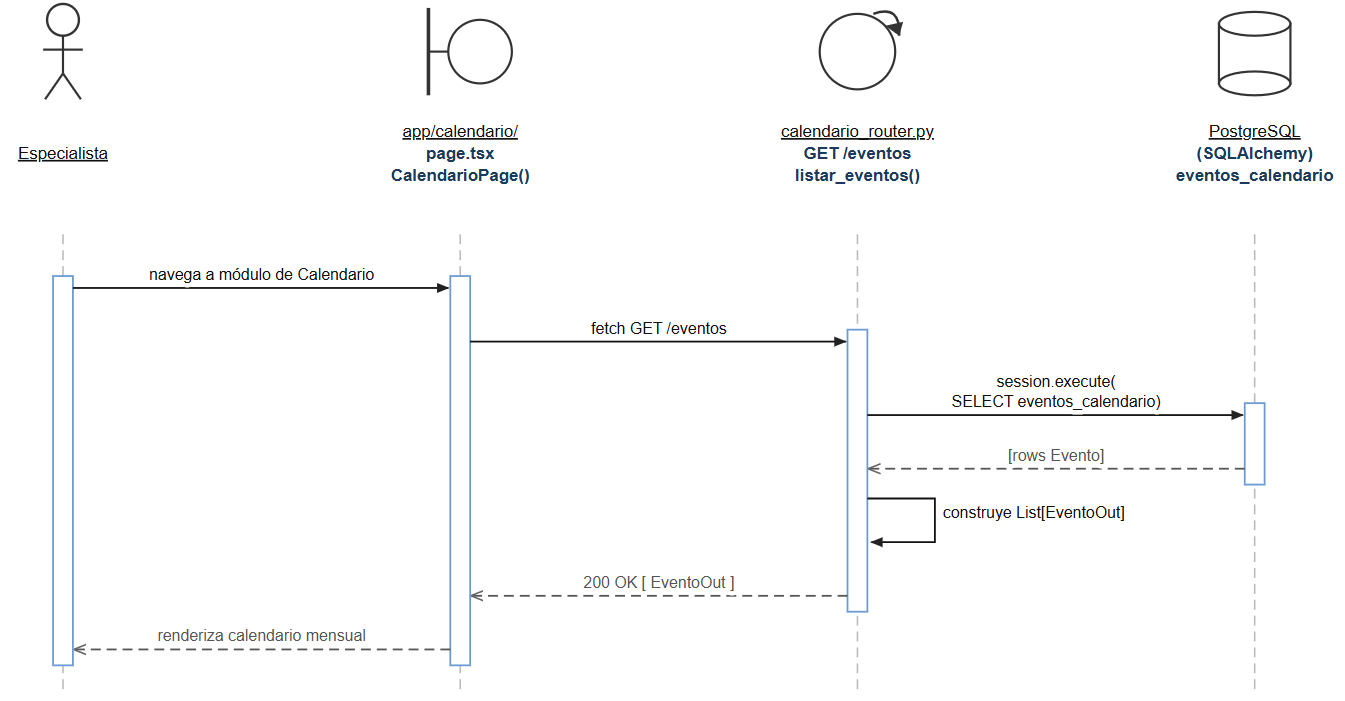
\includegraphics[width=0.8\textwidth]{img/CU38.png}
	\caption{Diagrama de secuencia --- CU-38 Consultar calendario de expedientes.}
	\label{fig:secuencia-cu38}
\end{figure}

\subsection*{Flujo Alternativo / Excepciones}
\begin{itemize}
	\item \textbf{E1: Sin eventos registrados en el periodo} - Si no existen actividades programadas en el mes consultado, el calendario se renderiza de forma limpia y vacía, notificando sutilmente que no hay eventos programados.
\end{itemize}

\bigskip
\noindent\rule{\linewidth}{0.5pt}
\bigskip

% ============================================================
\section{Diseño Dinámico del CU: Registrar evento en calendario (CU-39)}
% ============================================================

\subsection*{Descripción del Flujo}
El Especialista selecciona un día en el calendario y hace clic en "Añadir evento". Completa el formulario de programación de actividad (título, descripción, fecha y hora de inicio y fin, expediente del NNA y participantes). Al pulsar "Guardar", la interfaz envía la información al Backend. El Backend verifica en la base de datos que el expediente esté abierto y realiza una consulta para comprobar que los participantes clave no tengan otra actividad programada en el mismo intervalo de tiempo (evitando choques de agenda). Si la fecha está libre, inserta el evento en la base de datos y responde éxito. El evento aparece en el calendario.

\begin{figure}[H]
	\centering
	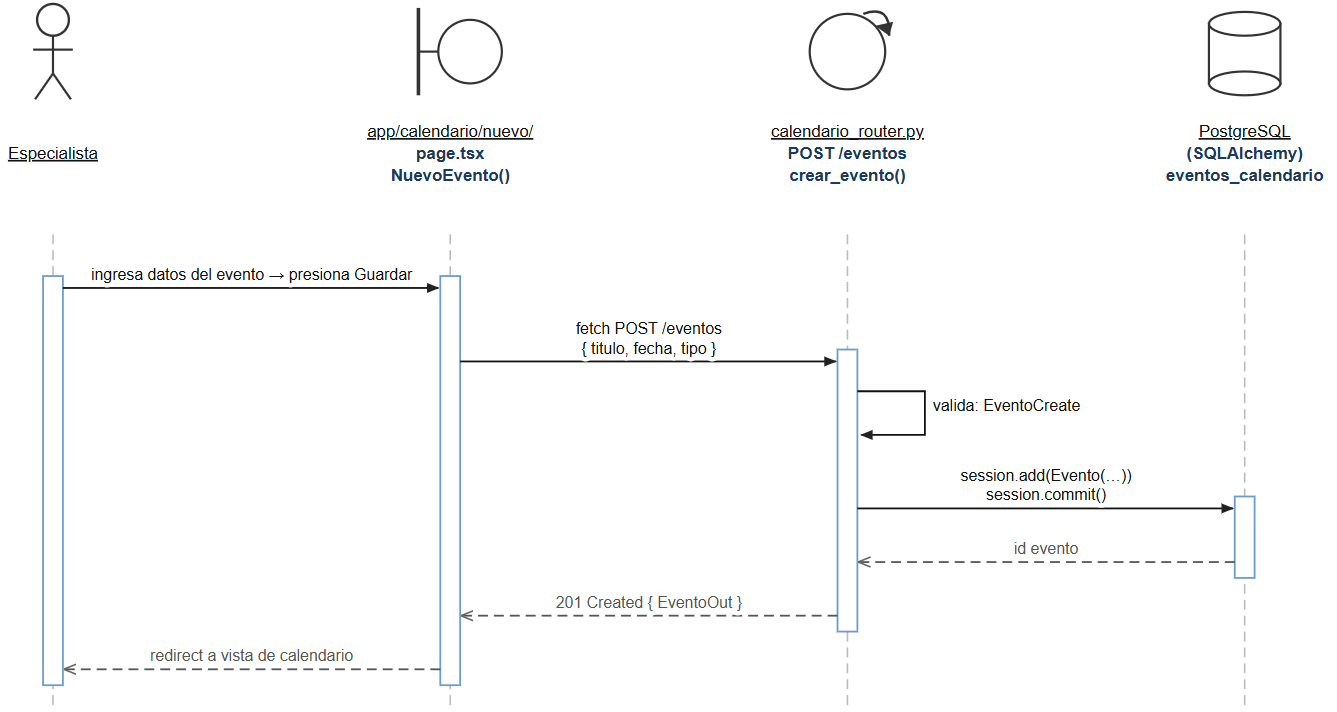
\includegraphics[width=0.8\textwidth]{img/CU39.png}
	\caption{Diagrama de secuencia --- CU-39 Registrar evento en calendario.}
	\label{fig:secuencia-cu39}
\end{figure}

\subsection*{Flujo Alternativo / Excepciones}
\begin{itemize}
	\item \textbf{E1: Conflicto de horario (choque de agenda)} - Uno de los especialistas o el expediente asociado ya tiene una actividad programada en el mismo horario seleccionado. El Backend aborta el registro y muestra la advertencia "El especialista o el expediente presenta un choque de horario".
	\item \textbf{E2: Expediente inactivo o cerrado} - Se intenta programar un evento para un expediente que ha sido archivado. El sistema bloquea el registro.
\end{itemize}

\bigskip
\noindent\rule{\linewidth}{0.5pt}
\bigskip

% ============================================================
\section{Diseño Dinámico del CU: Modificar evento en calendario (CU-40)}
% ============================================================

\subsection*{Descripción del Flujo}
El Especialista selecciona un evento en su calendario y presiona "Editar". Modifica el horario, fecha o participantes y guarda los cambios. El Backend recibe la solicitud, verifica la existencia del evento y ejecuta la validación de conflicto de horarios para el nuevo intervalo. Si no hay colisiones, actualiza el evento en la base de datos y devuelve éxito. La interfaz actualiza de inmediato la vista del calendario.

\begin{figure}[H]
	\centering
	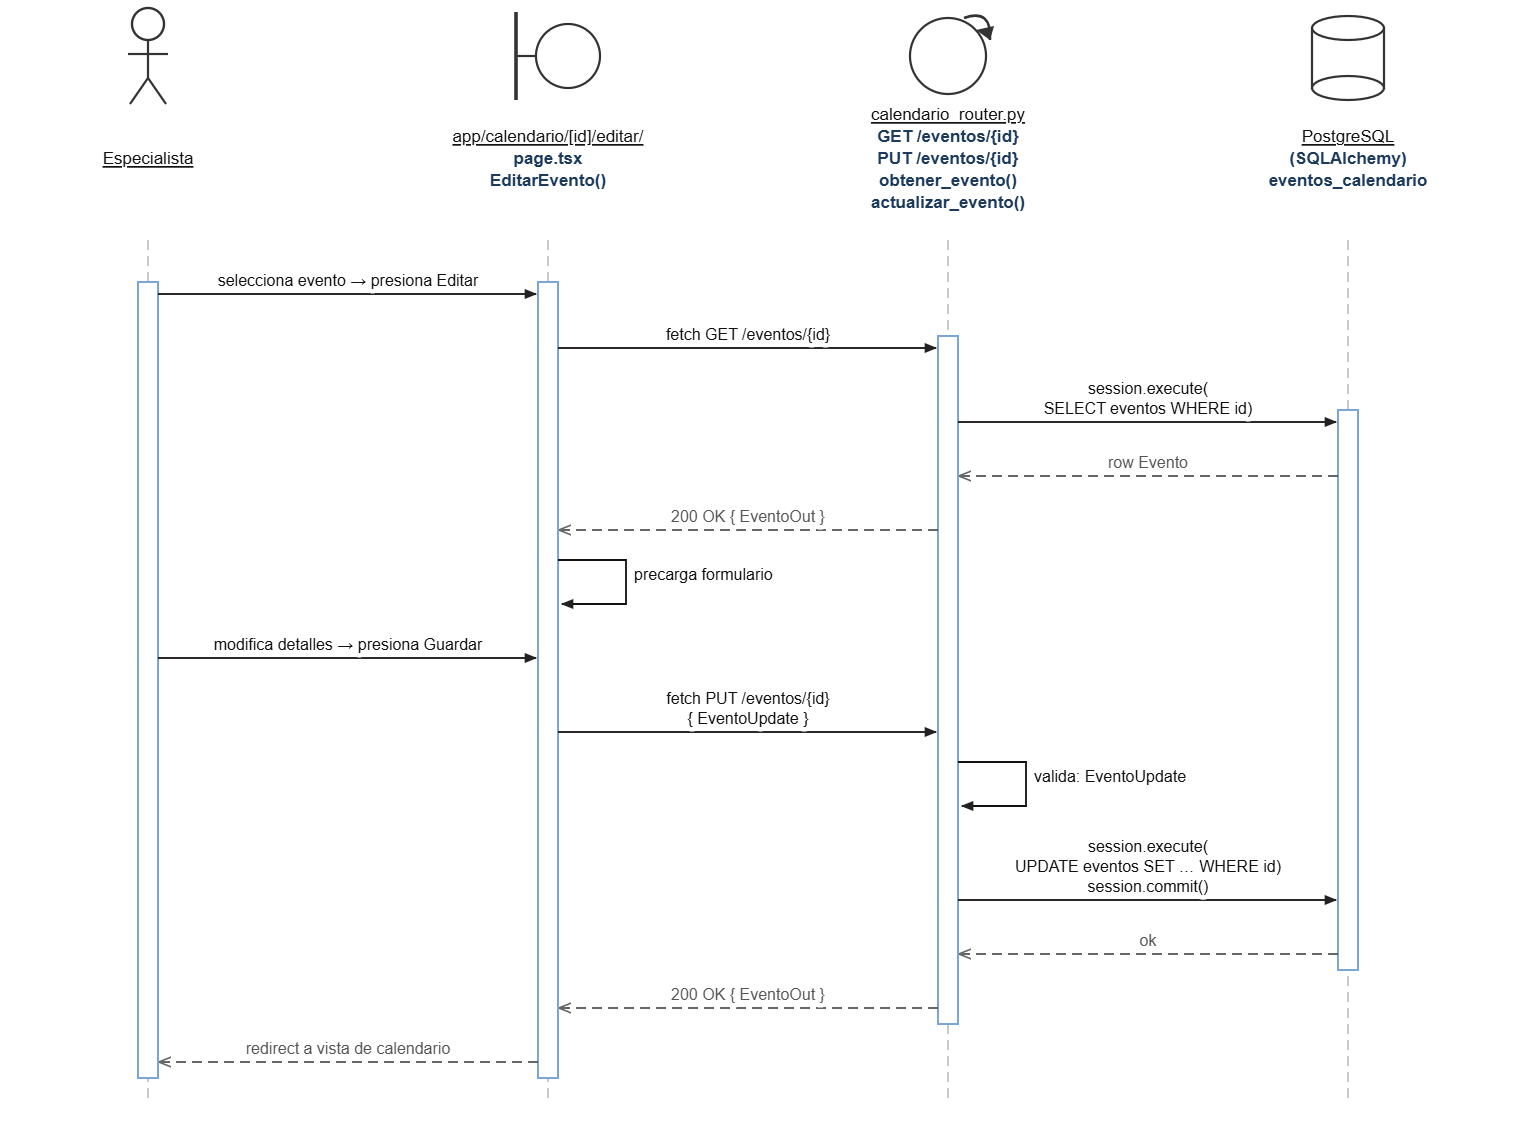
\includegraphics[width=0.8\textwidth]{img/CU-40.png}
	\caption{Diagrama de secuencia --- CU-40 Modificar evento en calendario.}
	\label{fig:secuencia-cu40}
\end{figure}

\subsection*{Flujo Alternativo / Excepciones}
\begin{itemize}
	\item \textbf{E1: Choque de agenda en el nuevo horario} - Los cambios propuestos causan conflicto de horario para alguno de los involucrados. El sistema cancela la actualización y muestra un mensaje de advertencia.
	\item \textbf{E2: Evento no encontrado o eliminado} - El evento a modificar fue cancelado o borrado previamente por otro especialista de forma simultánea. Se cancela el proceso y se notifica del estado.
\end{itemize}

\bigskip
\noindent\rule{\linewidth}{0.5pt}
\bigskip

% ============================================================
\section{Diseño Dinámico del CU: Registrar actor (CU-41)}
% ============================================================

\subsection*{Descripción del Flujo}
El Especialista accede al módulo del Directorio de Actores y presiona "Registrar Actor". Completa los datos de identidad. Si es Persona Física, captura el nombre, CURP, RFC, sexo, fecha de nacimiento y nivel de escolaridad. Si es Persona Moral/Organización, captura la razón social y el tipo de institución. Al guardar, la interfaz envía los datos al Backend. El Backend valida que los campos clave no estén vacíos y verifica en la base de datos que la CURP o el RFC no existan previamente. Si pasa las validaciones, inserta al actor en la base de datos con estado "Activo" y responde con éxito a la interfaz, que redirige al siguiente paso del registro (contactos).

\begin{figure}[H]
	\centering
	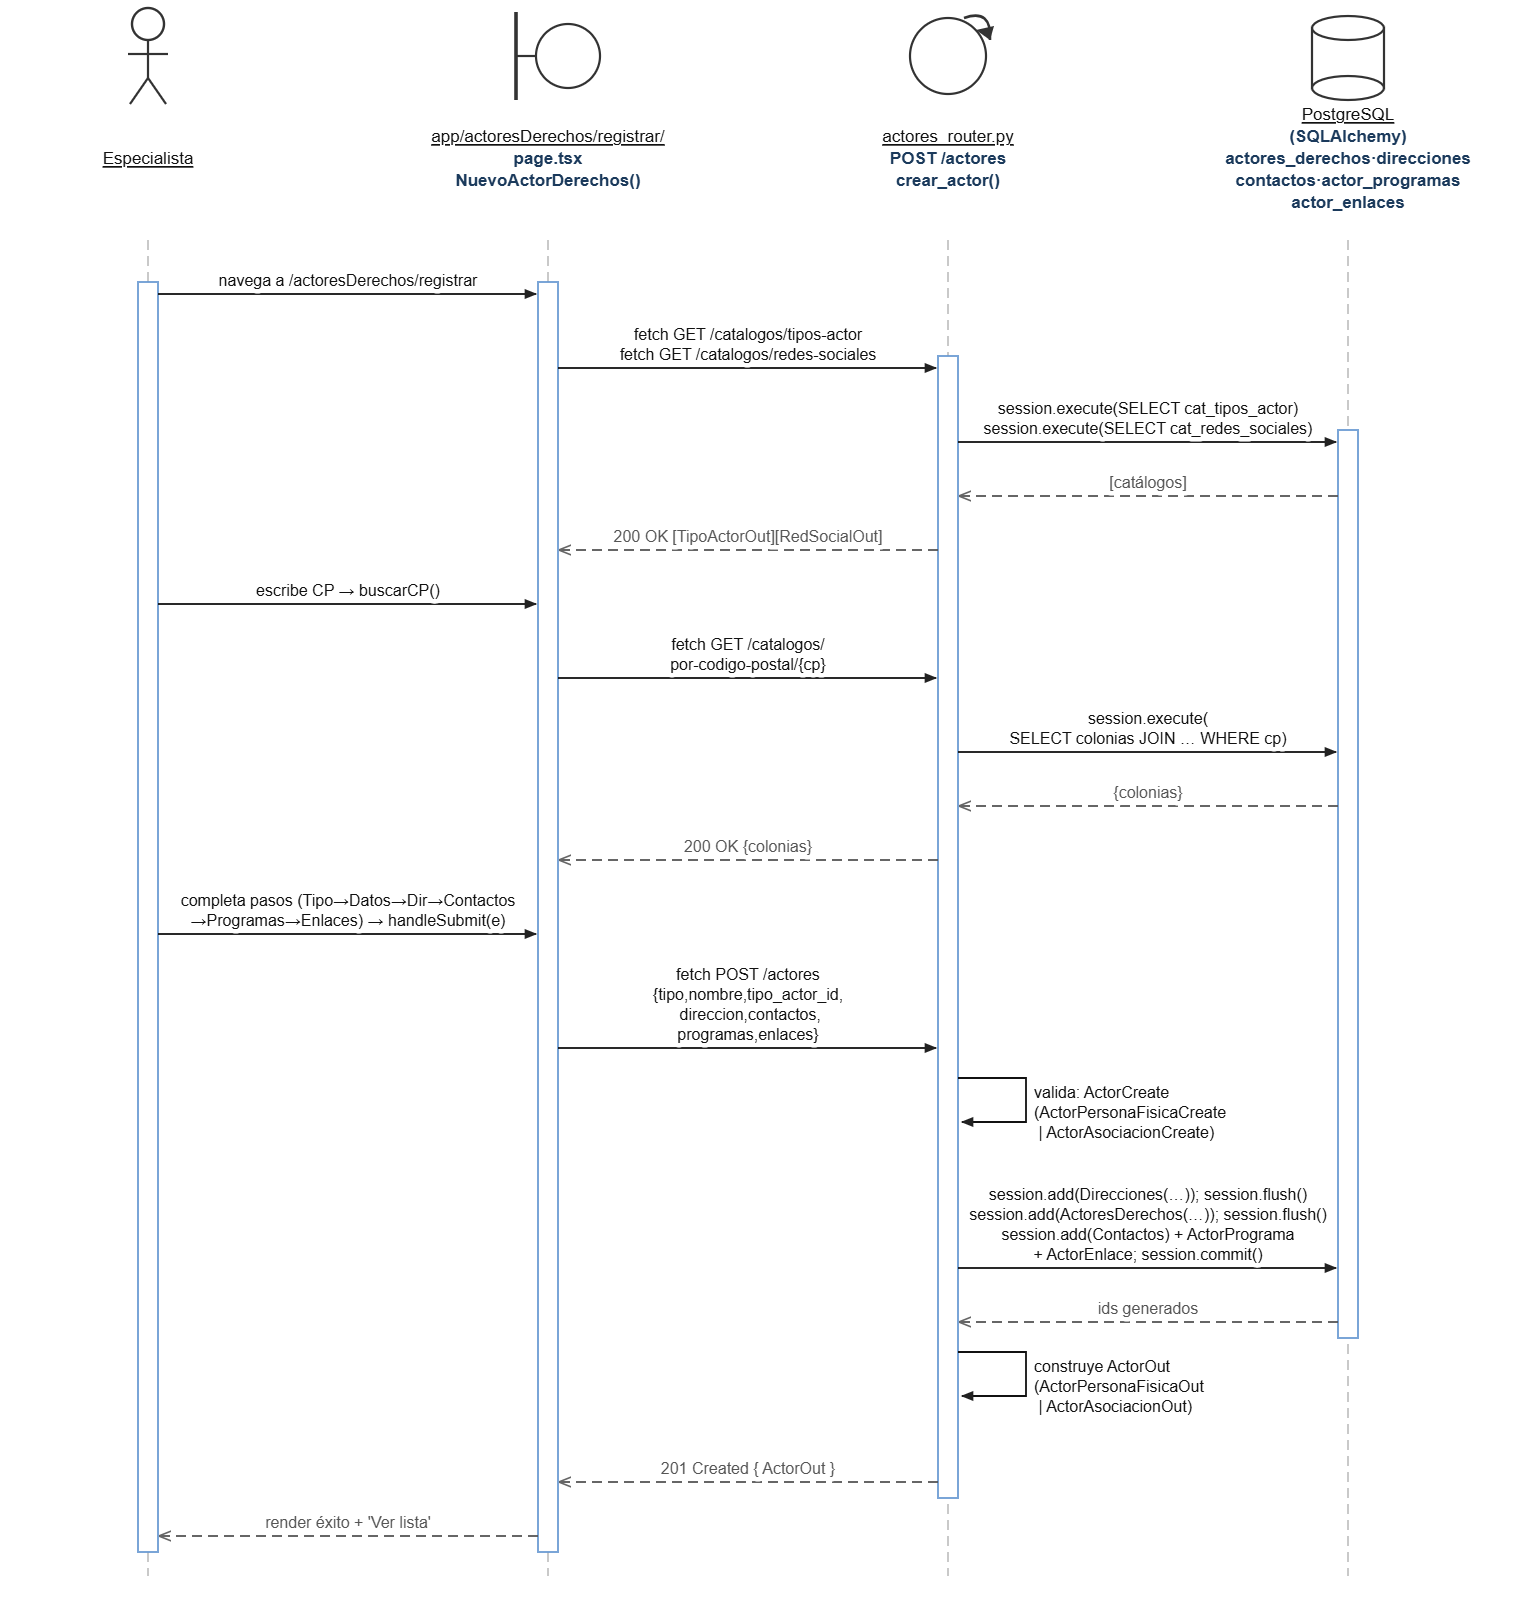
\includegraphics[width=0.8\textwidth]{img/CU-41.png}
	\caption{Diagrama de secuencia --- CU-41 Registrar actor.}
	\label{fig:secuencia-cu41}
\end{figure}

\subsection*{Flujo Alternativo / Excepciones}
\begin{itemize}
	\item \textbf{E1: CURP o RFC ya registrado} - El identificador legal (CURP o RFC) ya existe en el directorio de actores en la base de datos. El sistema bloquea el guardado e informa al usuario.
	\item \textbf{E2: Formato de identificador inválido} - La CURP o el RFC no cumplen con la longitud o estructura alfanumérica requerida. La interfaz detiene el proceso e indica el error en pantalla.
	\item \textbf{E3: Campos obligatorios incompletos} - Se omiten datos esenciales en el formulario de registro de actor. Se muestra un aviso de error.
\end{itemize}

\bigskip
\noindent\rule{\linewidth}{0.5pt}
\bigskip

% ============================================================
\section{Diseño Dinámico del CU: Registrar contactos del actor (CU-42)}
% ============================================================

\subsection*{Descripción del Flujo}
En la segunda fase del registro del actor, el Especialista ingresa los datos de contacto: teléfono principal, secundario, correo electrónico, sitio web y redes sociales. Al presionar "Guardar contactos", la interfaz valida los formatos de los campos de texto. El Backend recibe la información y la almacena en la tabla de contactos asociada al ID del actor en la base de datos. El Backend responde con éxito y la interfaz avanza al módulo de registro de ubicación.

\begin{figure}[H]
	\centering
	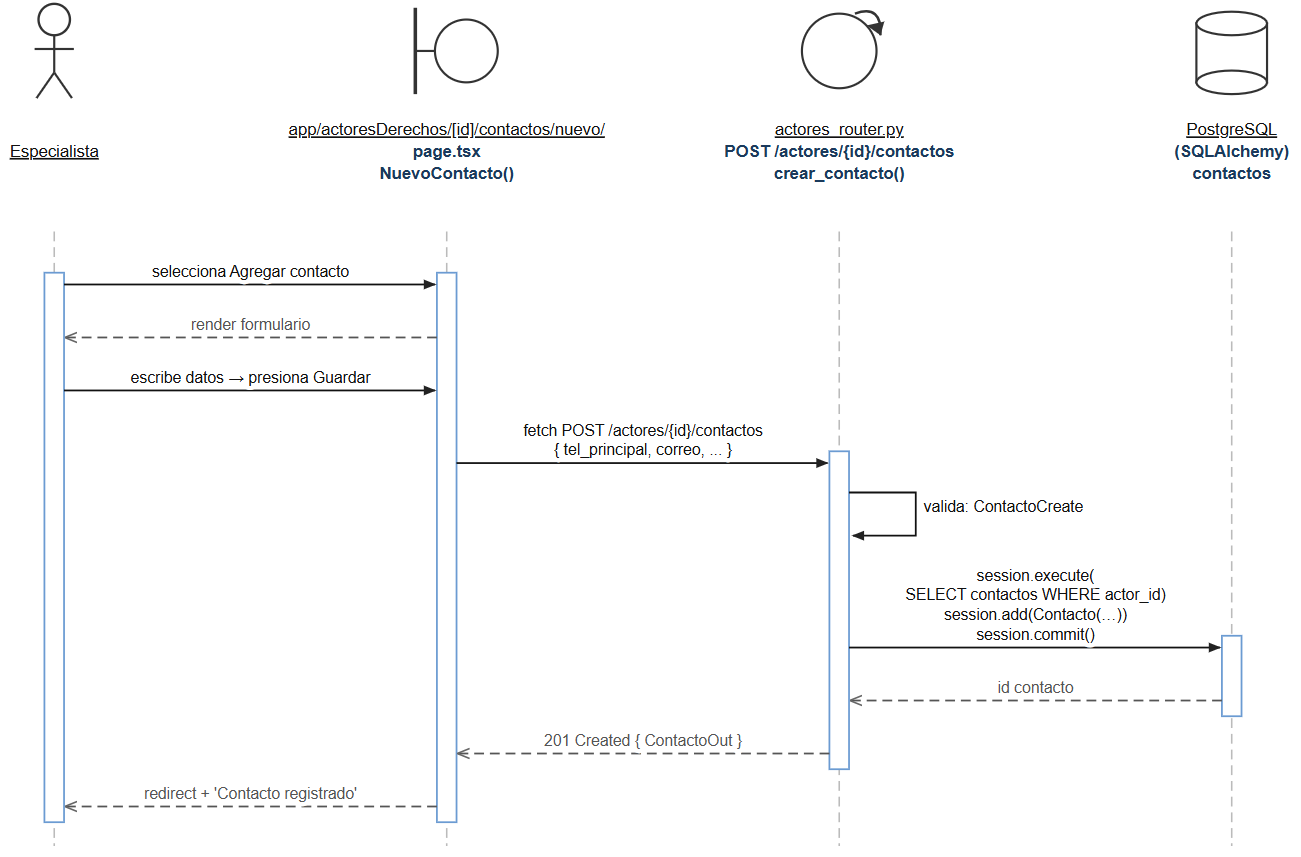
\includegraphics[width=0.8\textwidth]{img/CU42.png}
	\caption{Diagrama de secuencia --- CU-42 Registrar contactos del actor.}
	\label{fig:secuencia-cu42}
\end{figure}

\subsection*{Flujo Alternativo / Excepciones}
\begin{itemize}
	\item \textbf{E1: Correo electrónico inválido} - El formato del correo electrónico ingresado no cumple con el estándar. El sistema indica el error y cancela el guardado.
	\item \textbf{E2: Teléfono con formato incorrecto} - El número de teléfono contiene caracteres no permitidos o tiene una longitud inválida. Se bloquea el guardado y se resalta el campo.
\end{itemize}

\bigskip
\noindent\rule{\linewidth}{0.5pt}
\bigskip

% ============================================================
\section{Diseño Dinámico del CU: Registrar ubicación del actor (CU-43)}
% ============================================================

\subsection*{Descripción del Flujo}
En la tercera fase del registro del actor, el Especialista ingresa la dirección física de la sede o sucursal del actor. Digita el código postal, y la interfaz autocompleta el estado, municipio y lista de colonias gracias al catálogo SEPOMEX. El Especialista selecciona la colonia, captura la calle y los números exterior/interior y presiona "Guardar ubicación". El Backend guarda la dirección vinculada al actor en la base de datos. Tras recibir la confirmación de éxito del Backend, la interfaz avanza al paso de registro de programas.

\begin{figure}[H]
	\centering
	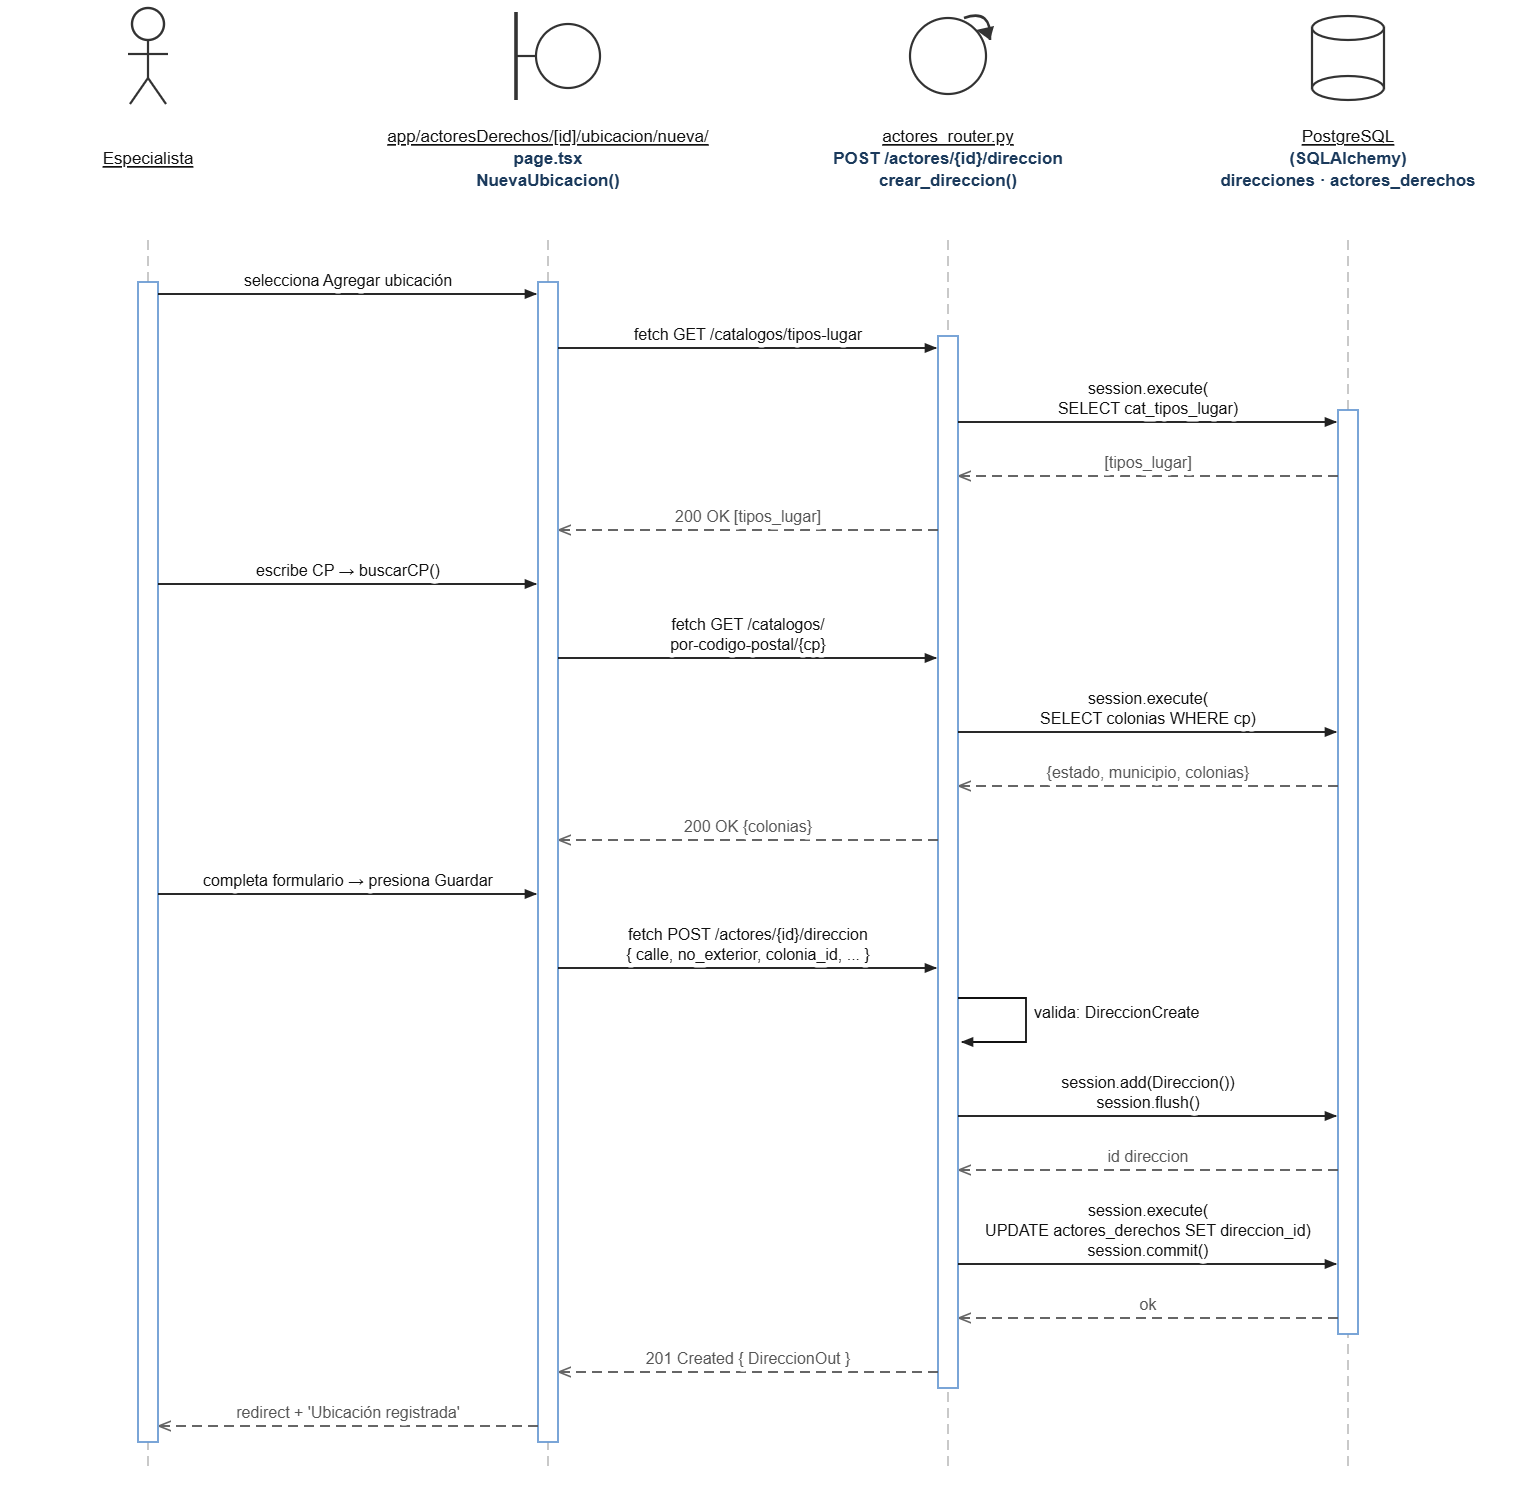
\includegraphics[width=0.8\textwidth]{img/CU-43.png}
	\caption{Diagrama de secuencia --- CU-43 Registrar ubicación del actor.}
	\label{fig:secuencia-cu43}
\end{figure}

\subsection*{Flujo Alternativo / Excepciones}
\begin{itemize}
	\item \textbf{E1: Código postal no encontrado} - El CP no se encuentra en el catálogo SEPOMEX del sistema. Se advierte de la situación y se habilita la edición manual de los campos de dirección.
	\item \textbf{E2: Datos obligatorios de dirección ausentes} - Se omite capturar la calle o el número exterior. La interfaz bloquea el envío y resalta las carencias.
\end{itemize}

\bigskip
\noindent\rule{\linewidth}{0.5pt}
\bigskip

% ============================================================
\section{Diseño Dinámico del CU: Registrar programas del actor (CU-44)}
% ============================================================

\subsection*{Descripción del Flujo}
En la cuarta fase del registro del actor, el Especialista captura los programas de apoyo que este ofrece al NNA. Introduce el nombre del programa, su descripción, y los servicios específicos incluidos, definiendo el costo (o si es de gratuidad completa), duración de la atención y requisitos de admisión. Al guardar, la interfaz envía los datos al Backend. El Backend almacena los programas y servicios vinculados al actor en la base de datos y devuelve éxito. La interfaz avanza a la última fase (enlaces representantes).

\begin{figure}[H]
	\centering
	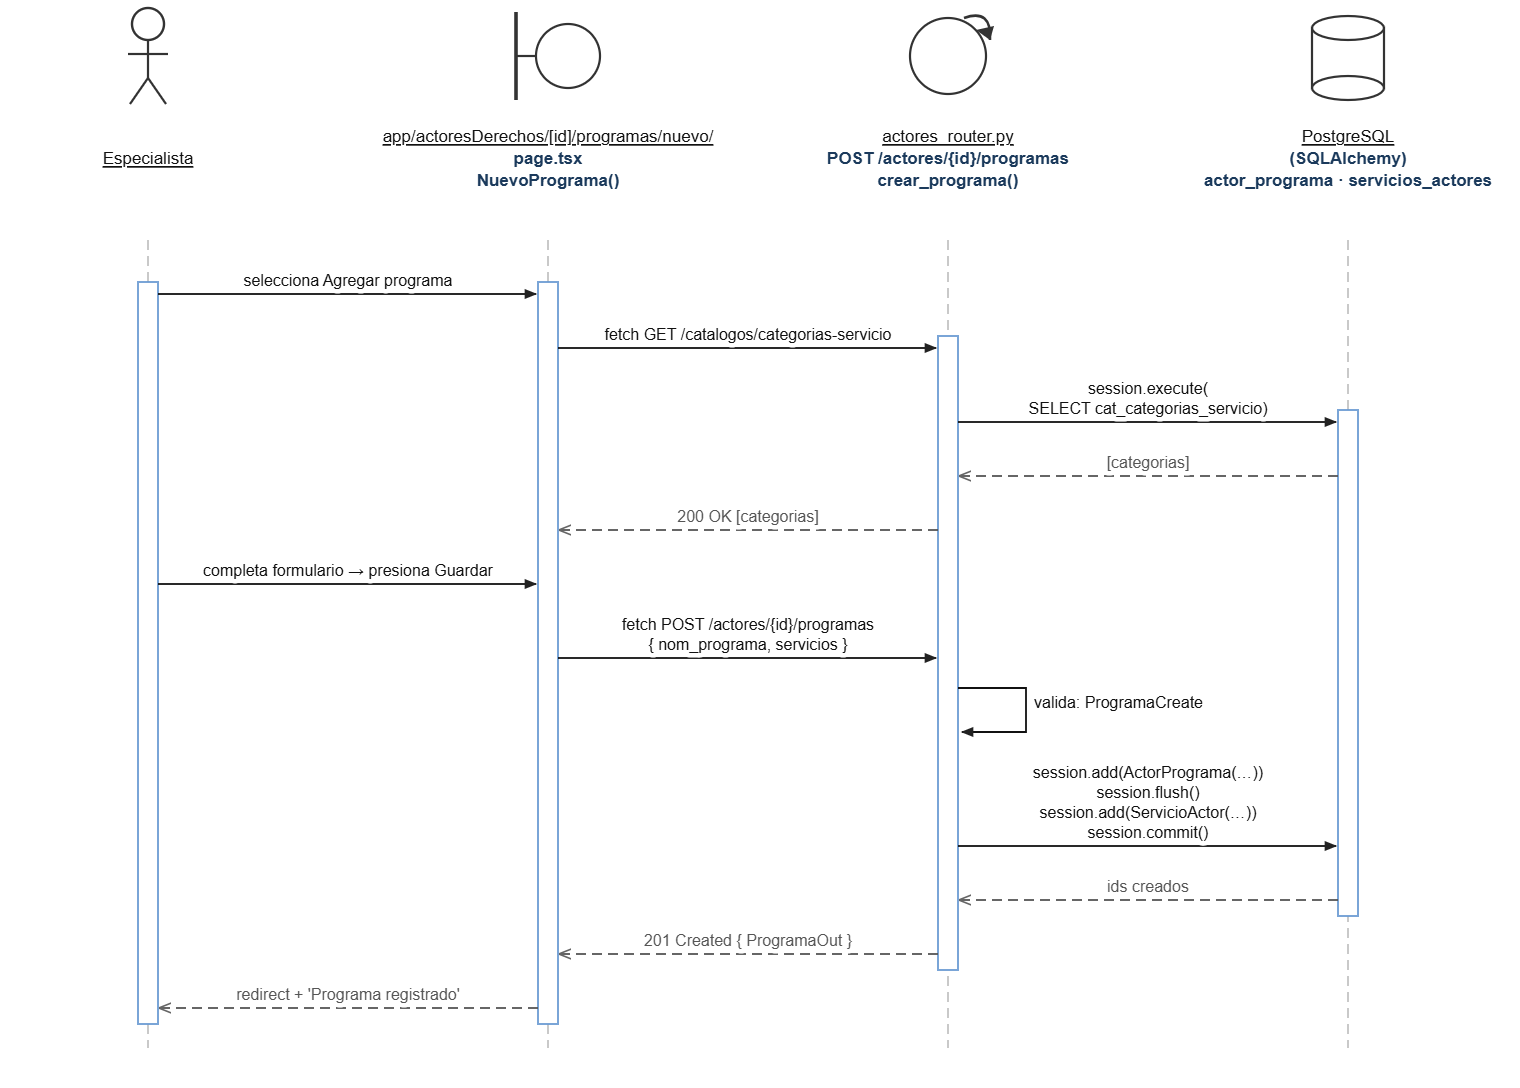
\includegraphics[width=0.8\textwidth]{img/CU-44.png}
	\caption{Diagrama de secuencia --- CU-44 Registrar programas del actor.}
	\label{fig:secuencia-cu44}
\end{figure}

\subsection*{Flujo Alternativo / Excepciones}
\begin{itemize}
	\item \textbf{E1: Nombre del programa o servicio en blanco} - Se intenta guardar el programa omitiendo su nombre o el de sus servicios. El sistema muestra una alerta de error.
	\item \textbf{E2: Servicio no gratuito sin costo especificado} - Si se marca que el servicio tiene un costo pero se deja en blanco el monto. Se bloquea el registro y se solicita capturar la cantidad.
\end{itemize}

\bigskip
\noindent\rule{\linewidth}{0.5pt}
\bigskip

% ============================================================
\section{Diseño Dinámico del CU: Registrar enlaces representantes (CU-45)}
% ============================================================

\subsection*{Descripción del Flujo}
En la fase final del registro del actor, el Especialista captura la información del personal que funge como enlace o representante institucional (nombre completo, cargo, teléfono y correo electrónico de contacto). Al pulsar "Finalizar registro", la interfaz envía los datos al Backend. El Backend guarda la información de los representantes en la base de datos, marca el registro global del actor como "Completado" y devuelve confirmación exitosa. La interfaz muestra un mensaje de éxito general y redirige al listado del directorio.

\begin{figure}[H]
	\centering
	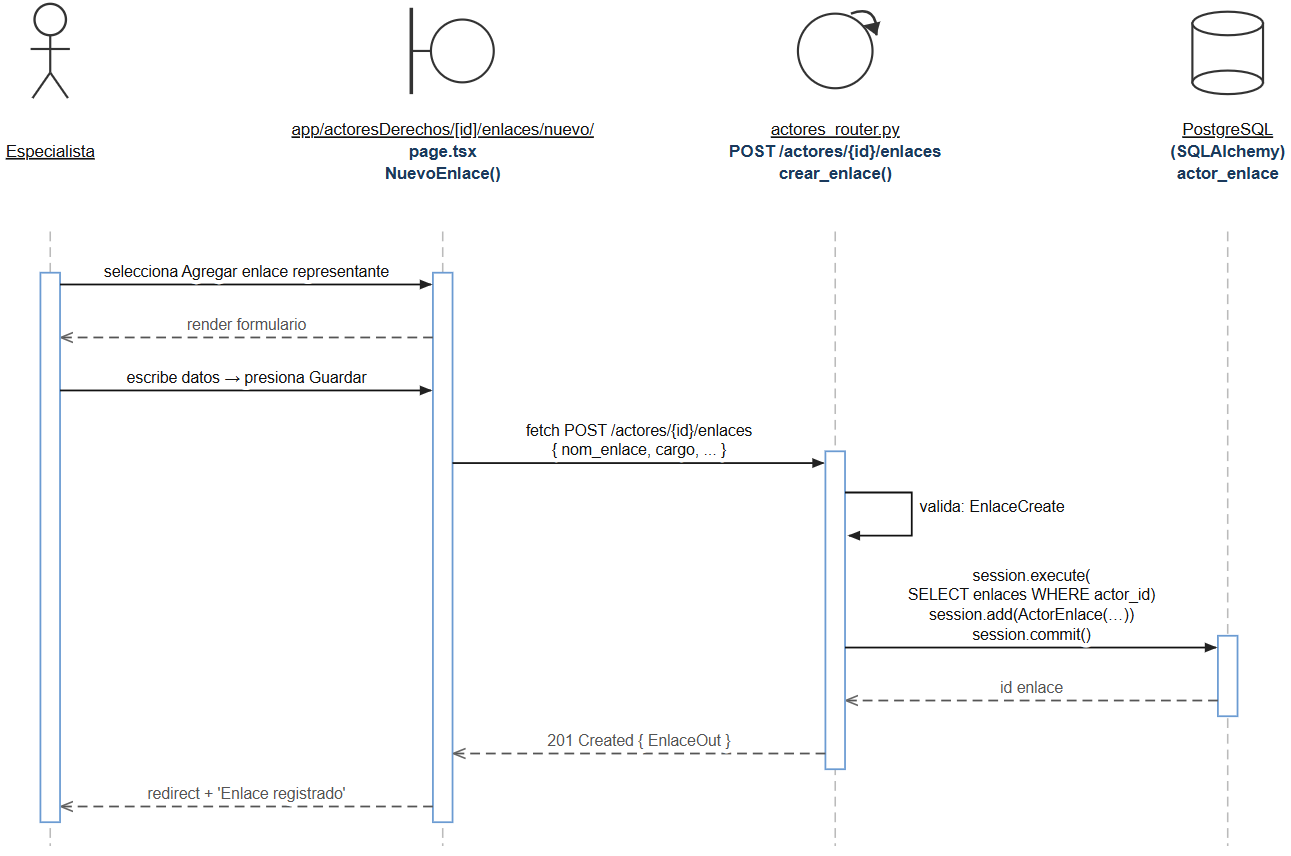
\includegraphics[width=0.8\textwidth]{img/CU45.png}
	\caption{Diagrama de secuencia --- CU-45 Registrar enlaces representantes.}
	\label{fig:secuencia-cu45}
\end{figure}

\subsection*{Flujo Alternativo / Excepciones}
\begin{itemize}
	\item \textbf{E1: Datos de contacto del enlace inválidos} - El correo o teléfono del enlace contiene errores de formato. El sistema cancela el guardado e indica el error.
	\item \textbf{E2: Nombre del enlace ausente} - No se ingresó el nombre de la persona de contacto. Se bloquea la finalización.
\end{itemize}

\bigskip
\noindent\rule{\linewidth}{0.5pt}
\bigskip

% ============================================================
\section{Diseño Dinámico del CU: Buscar actores (CU-46)}
% ============================================================

\subsection*{Descripción del Flujo}
El Especialista ingresa al Directorio de Actores y escribe un término de búsqueda (nombre del actor, municipio o tipo de apoyo) en el filtro. La interfaz envía los criterios de búsqueda al Backend. El Backend realiza una consulta filtrada en la base de datos sobre la tabla de actores utilizando operadores relacionales y de texto. La base de datos devuelve la lista de actores activos coincidentes. El Backend transmite los registros a la interfaz, que dibuja los resultados en pantalla.

\begin{figure}[H]
	\centering
	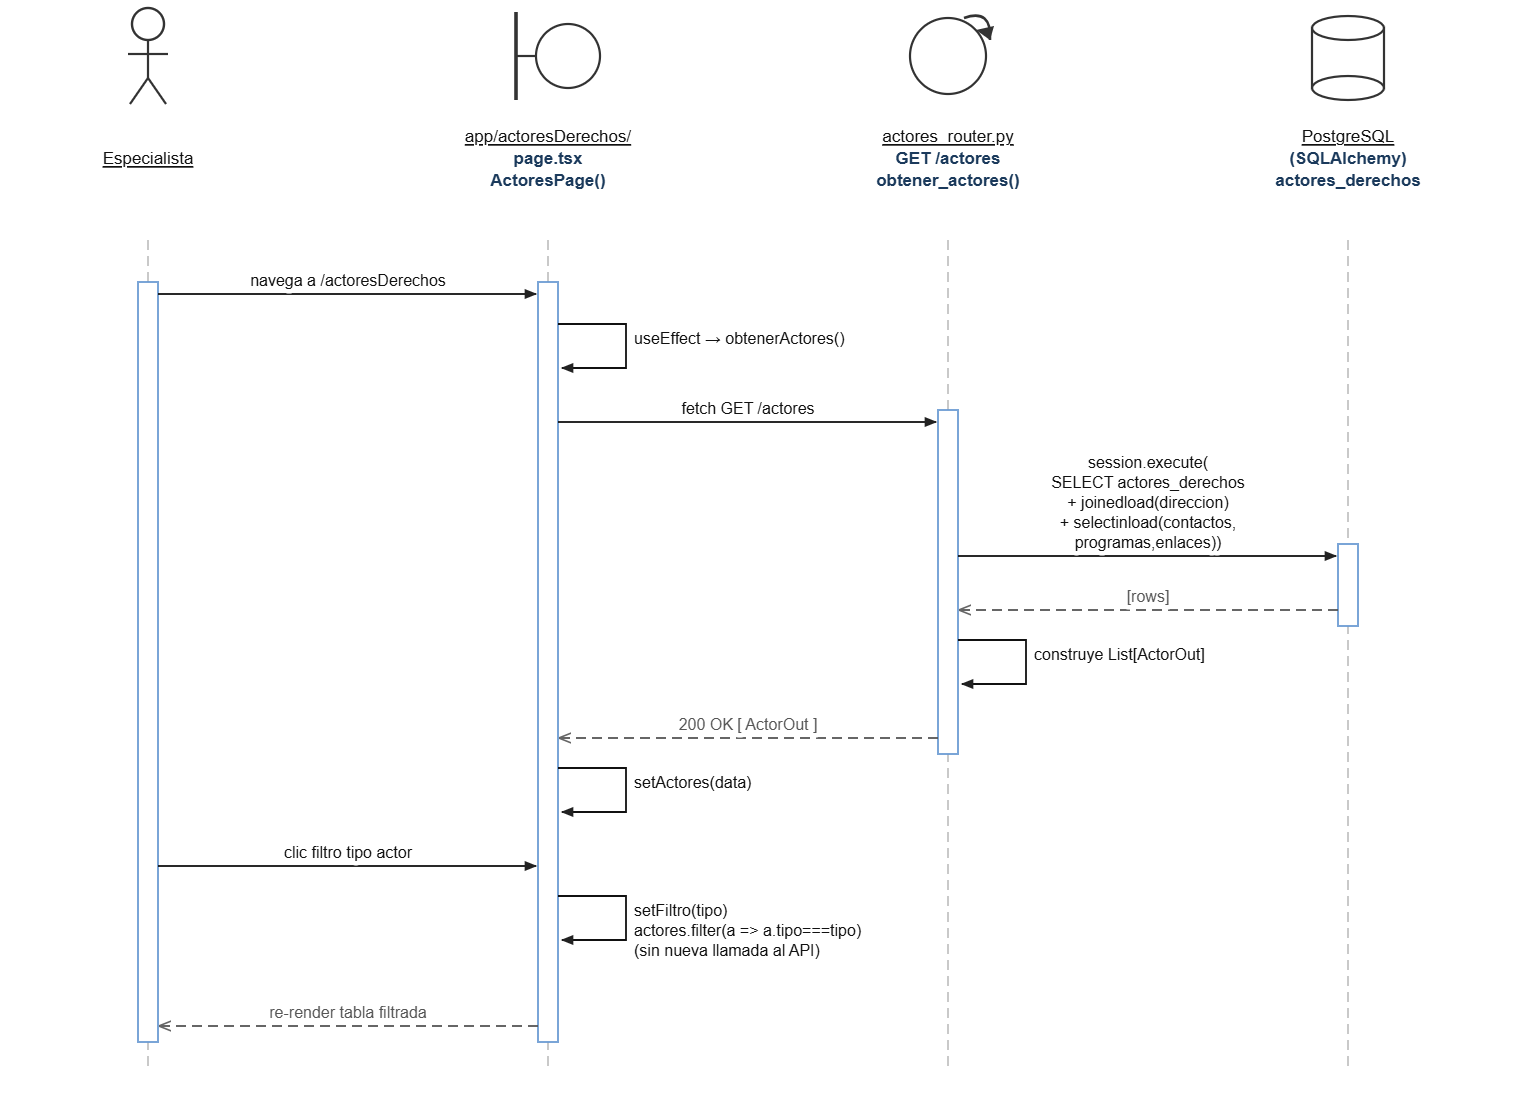
\includegraphics[width=0.8\textwidth]{img/CU-46.png}
	\caption{Diagrama de secuencia --- CU-46 Buscar actores.}
	\label{fig:secuencia-cu46}
\end{figure}

\subsection*{Flujo Alternativo / Excepciones}
\begin{itemize}
	\item \textbf{E1: Sin resultados coincidentes} - Ningún actor registrado en la base de datos coincide con los criterios de búsqueda provistos. El sistema muestra un mensaje indicando que no se encontraron coincidencias.
\end{itemize}

\bigskip
\noindent\rule{\linewidth}{0.5pt}
\bigskip

% ============================================================
\section{Diseño Dinámico del CU: Filtrar actores por tipo (CU-47)}
% ============================================================

\subsection*{Descripción del Flujo}
En la pantalla de visualización del Directorio de Actores, el Especialista despliega el menú de filtros y selecciona "Persona Física" o "Persona Moral / Institución". La interfaz procesa el filtro y solicita la lista depurada al Backend. El Backend realiza una consulta select condicional en la base de datos filtrando los registros por el tipo de actor seleccionado. La base de datos devuelve los registros correspondientes y el Backend los transmite a la interfaz, que refresca instantáneamente la lista de actores en pantalla.

\begin{figure}[H]
	\centering
	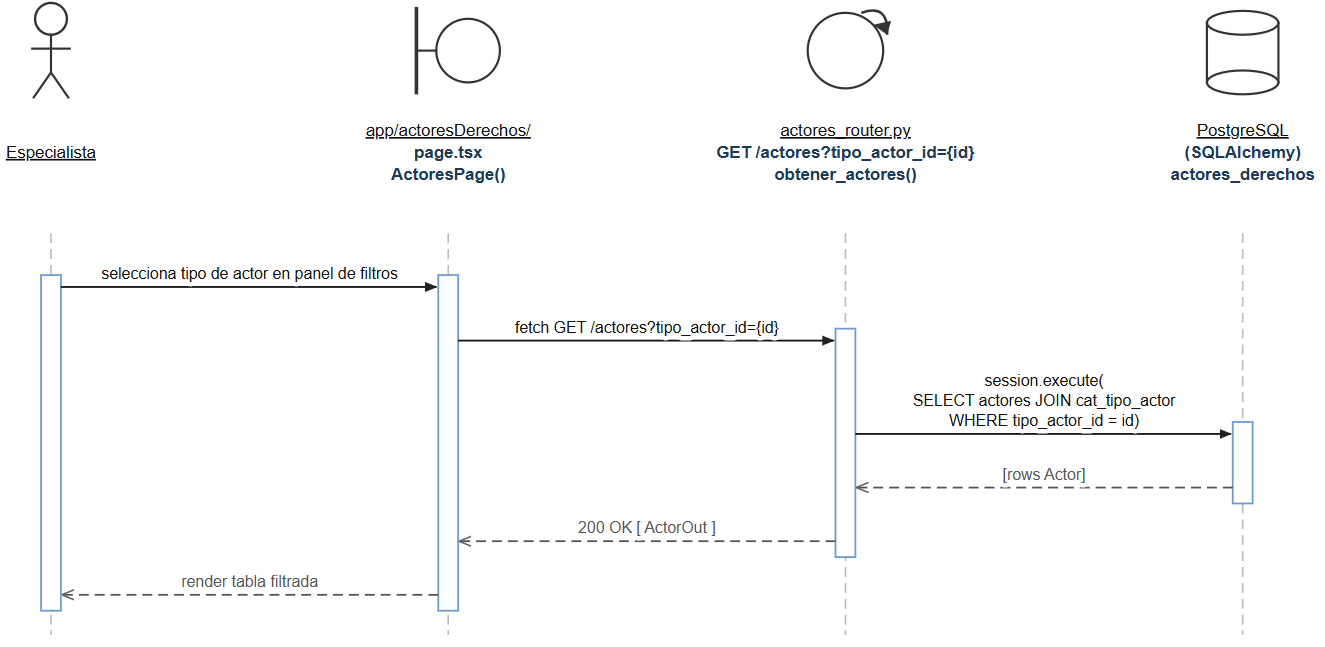
\includegraphics[width=0.8\textwidth]{img/CU47.png}
	\caption{Diagrama de secuencia --- CU-47 Filtrar actores por tipo.}
	\label{fig:secuencia-cu47}
\end{figure}

\subsection*{Flujo Alternativo / Excepciones}
\begin{itemize}
	\item \textbf{E1: No existen actores del tipo seleccionado} - Si la base de datos no contiene registros del tipo de actor elegido, el listado se muestra limpio e indica que no hay actores de ese tipo registrados.
\end{itemize}

\bigskip
\noindent\rule{\linewidth}{0.5pt}
\bigskip

% ============================================================
\section{Diseño Dinámico del CU: Consultar actor (CU-48)}
% ============================================================

\subsection*{Descripción del Flujo}
El Especialista selecciona un actor del listado en el directorio. La interfaz solicita los datos detallados del actor al Backend. El Backend realiza una serie de consultas indexadas en la base de datos para recuperar toda la información vinculada al actor: datos de identidad, contactos registrados, ubicaciones geográficas, programas y servicios ofertados, y enlaces representantes. La base de datos devuelve la información estructurada. El Backend organiza los datos y los envía a la interfaz, que los renderiza de forma limpia y ordenada en pestañas temáticas.

\begin{figure}[H]
	\centering
	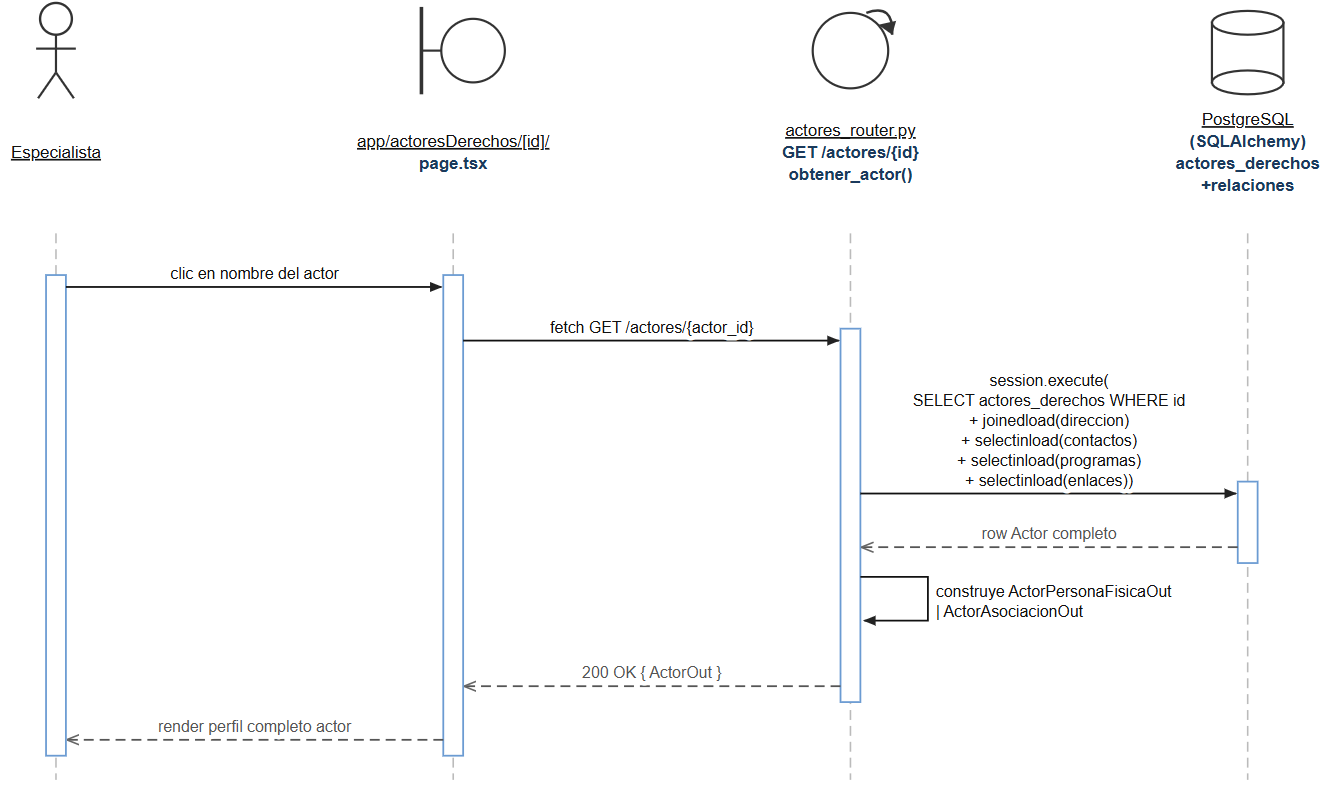
\includegraphics[width=0.8\textwidth]{img/CU48.png}
	\caption{Diagrama de secuencia --- CU-48 Consultar actor.}
	\label{fig:secuencia-cu48}
\end{figure}

\subsection*{Flujo Alternativo / Excepciones}
\begin{itemize}
	\item \textbf{E1: Actor inhabilitado o inexistente} - El identificador del actor consultado no corresponde a ningún registro activo. Se deniega la visualización y se redirige al listado con un mensaje de error.
\end{itemize}

\bigskip
\noindent\rule{\linewidth}{0.5pt}
\bigskip

% ============================================================
\section{Diseño Dinámico del CU: Editar actor (CU-49)}
% ============================================================

\subsection*{Descripción del Flujo}
El Especialista visualiza el perfil de un actor y presiona "Editar Identidad". Modifica los datos generales (nombre, tipo de organización, etc.) en el formulario de edición y pulsa "Guardar". La interfaz transmite los datos al Backend. El Backend valida que los datos no generen conflictos (comprobando que la CURP o RFC no colisionen con los de otro actor registrado en la base de datos) y actualiza la información del actor en la base de datos, retornando éxito. La interfaz actualiza el perfil del actor.

\begin{figure}[H]
	\centering
	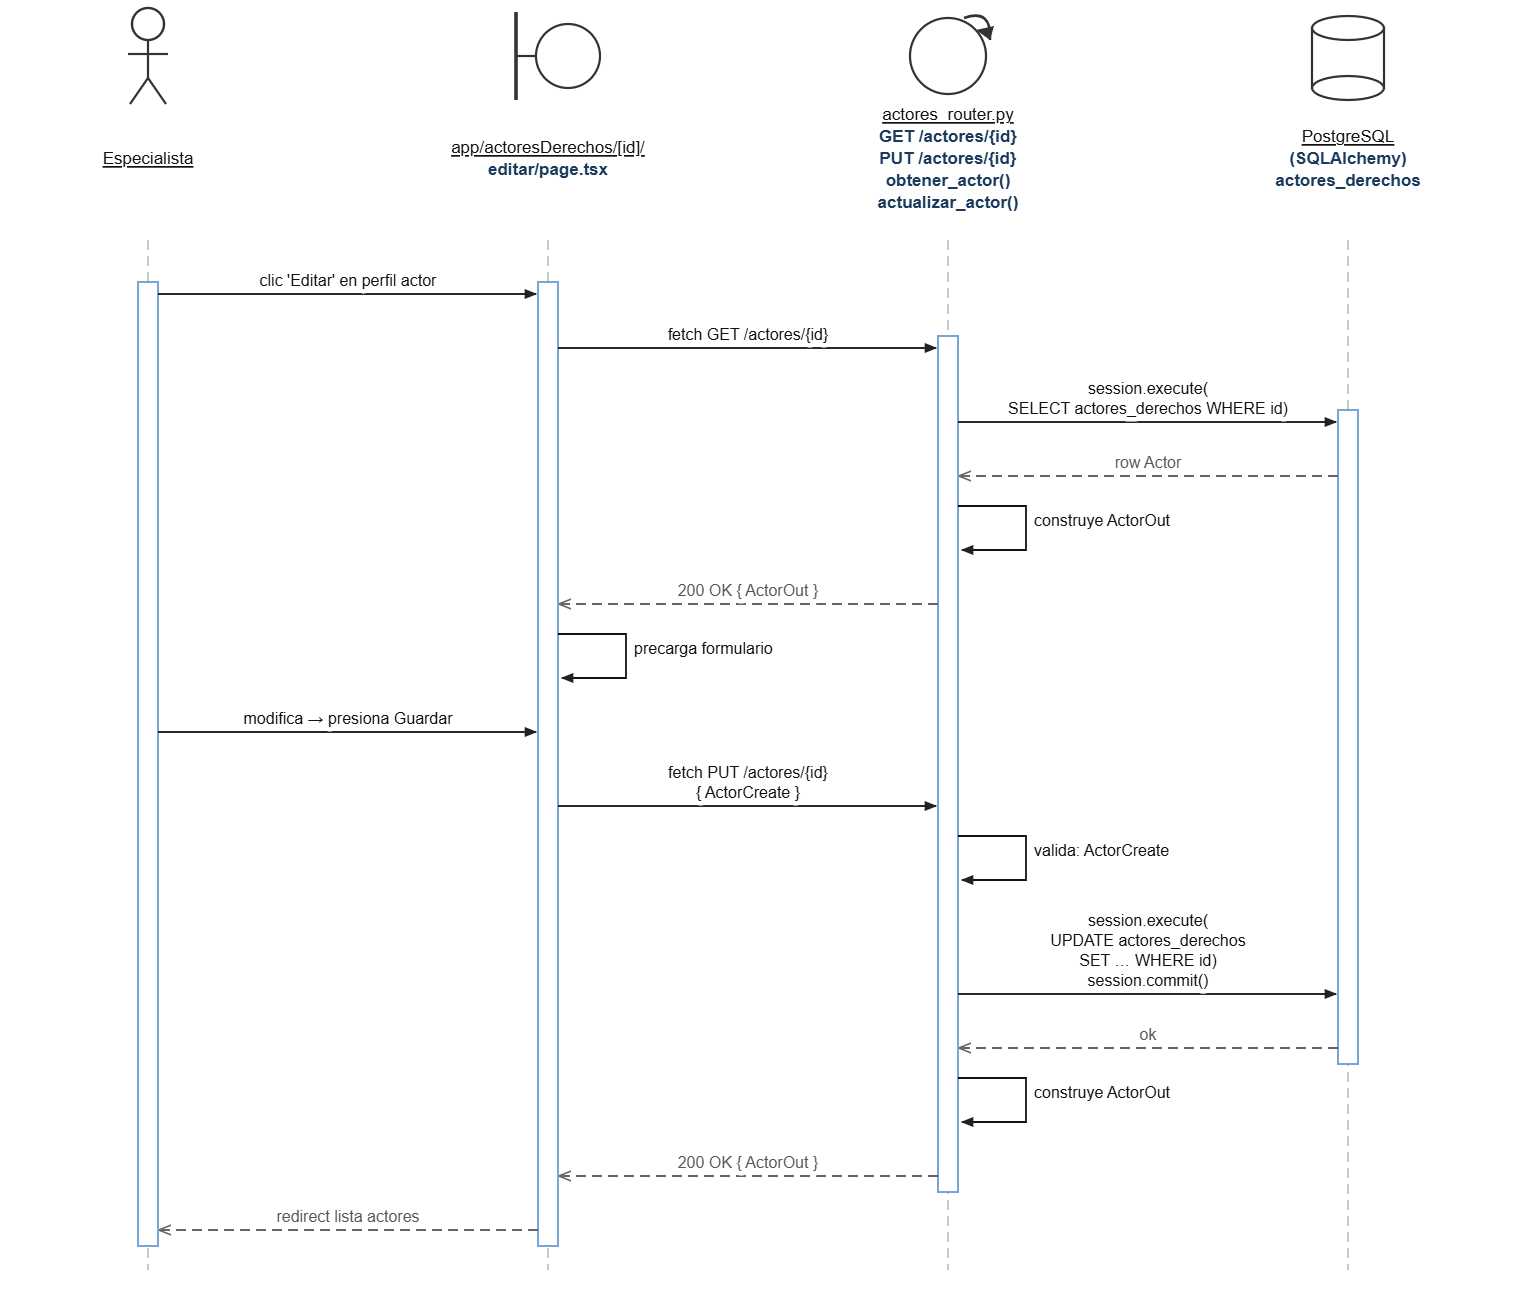
\includegraphics[width=0.8\textwidth]{img/CU-49.png}
	\caption{Diagrama de secuencia --- CU-49 Editar actor.}
	\label{fig:secuencia-cu49}
\end{figure}

\subsection*{Flujo Alternativo / Excepciones}
\begin{itemize}
	\item \textbf{E1: Identificador legal duplicado} - El RFC o la CURP modificada ya se encuentra registrada para otro actor en la base de datos. El sistema bloquea el guardado e informa del error.
	\item \textbf{E2: Campos obligatorios en blanco} - El usuario borra información esencial. La interfaz detiene el guardado y resalta las omisiones.
\end{itemize}

\bigskip
\noindent\rule{\linewidth}{0.5pt}
\bigskip

% ============================================================
\section{Diseño Dinámico del CU: Editar contactos del actor (CU-50)}
% ============================================================

\subsection*{Descripción del Flujo}
El Especialista accede a la sección de contactos en el perfil del actor y presiona "Editar Contactos". Actualiza los números telefónicos, correos electrónicos o redes sociales del actor y pulsa "Guardar". El Backend recibe la solicitud, valida los formatos y aplica los cambios en la tabla de contactos de la base de datos. Finalmente, responde con éxito y la interfaz actualiza los datos en pantalla.

\begin{figure}[H]
	\centering
	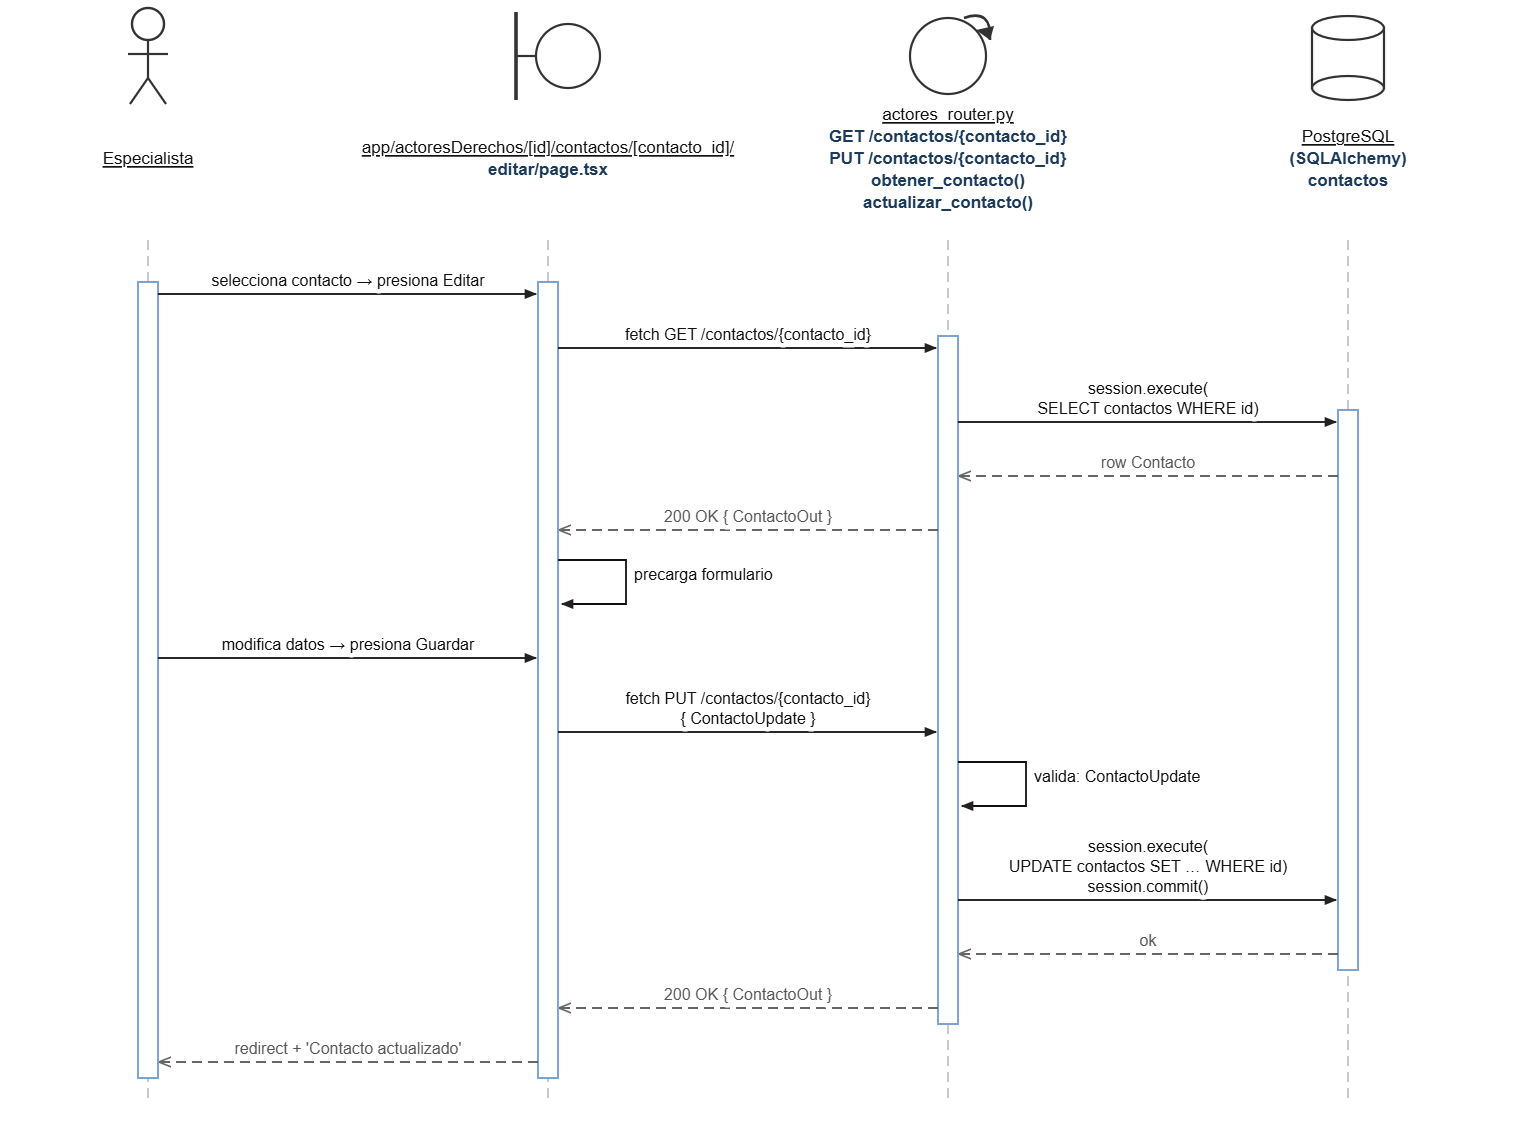
\includegraphics[width=0.8\textwidth]{img/CU-50.png}
	\caption{Diagrama de secuencia --- CU-50 Editar contactos del actor.}
	\label{fig:secuencia-cu50}
\end{figure}

\subsection*{Flujo Alternativo / Excepciones}
\begin{itemize}
	\item \textbf{E1: Formato de correo o teléfono incorrecto} - Los nuevos datos de contacto contienen errores estructurales. El sistema bloquea la actualización y solicita su corrección.
\end{itemize}

\bigskip
\noindent\rule{\linewidth}{0.5pt}
\bigskip

% ============================================================
\section{Diseño Dinámico del CU: Editar ubicación del actor (CU-51)}
% ============================================================

\subsection*{Descripción del Flujo}
El Especialista accede a la sección de ubicaciones del actor y selecciona "Editar Ubicación". Modifica los campos de dirección y el código postal, y el catálogo SEPOMEX actualiza dinámicamente las colonias en pantalla. Tras guardar los cambios, la interfaz envía los datos al Backend. El Backend actualiza el registro de dirección en la base de datos y responde confirmando éxito. La interfaz muestra un aviso de guardado exitoso.

\begin{figure}[H]
	\centering
	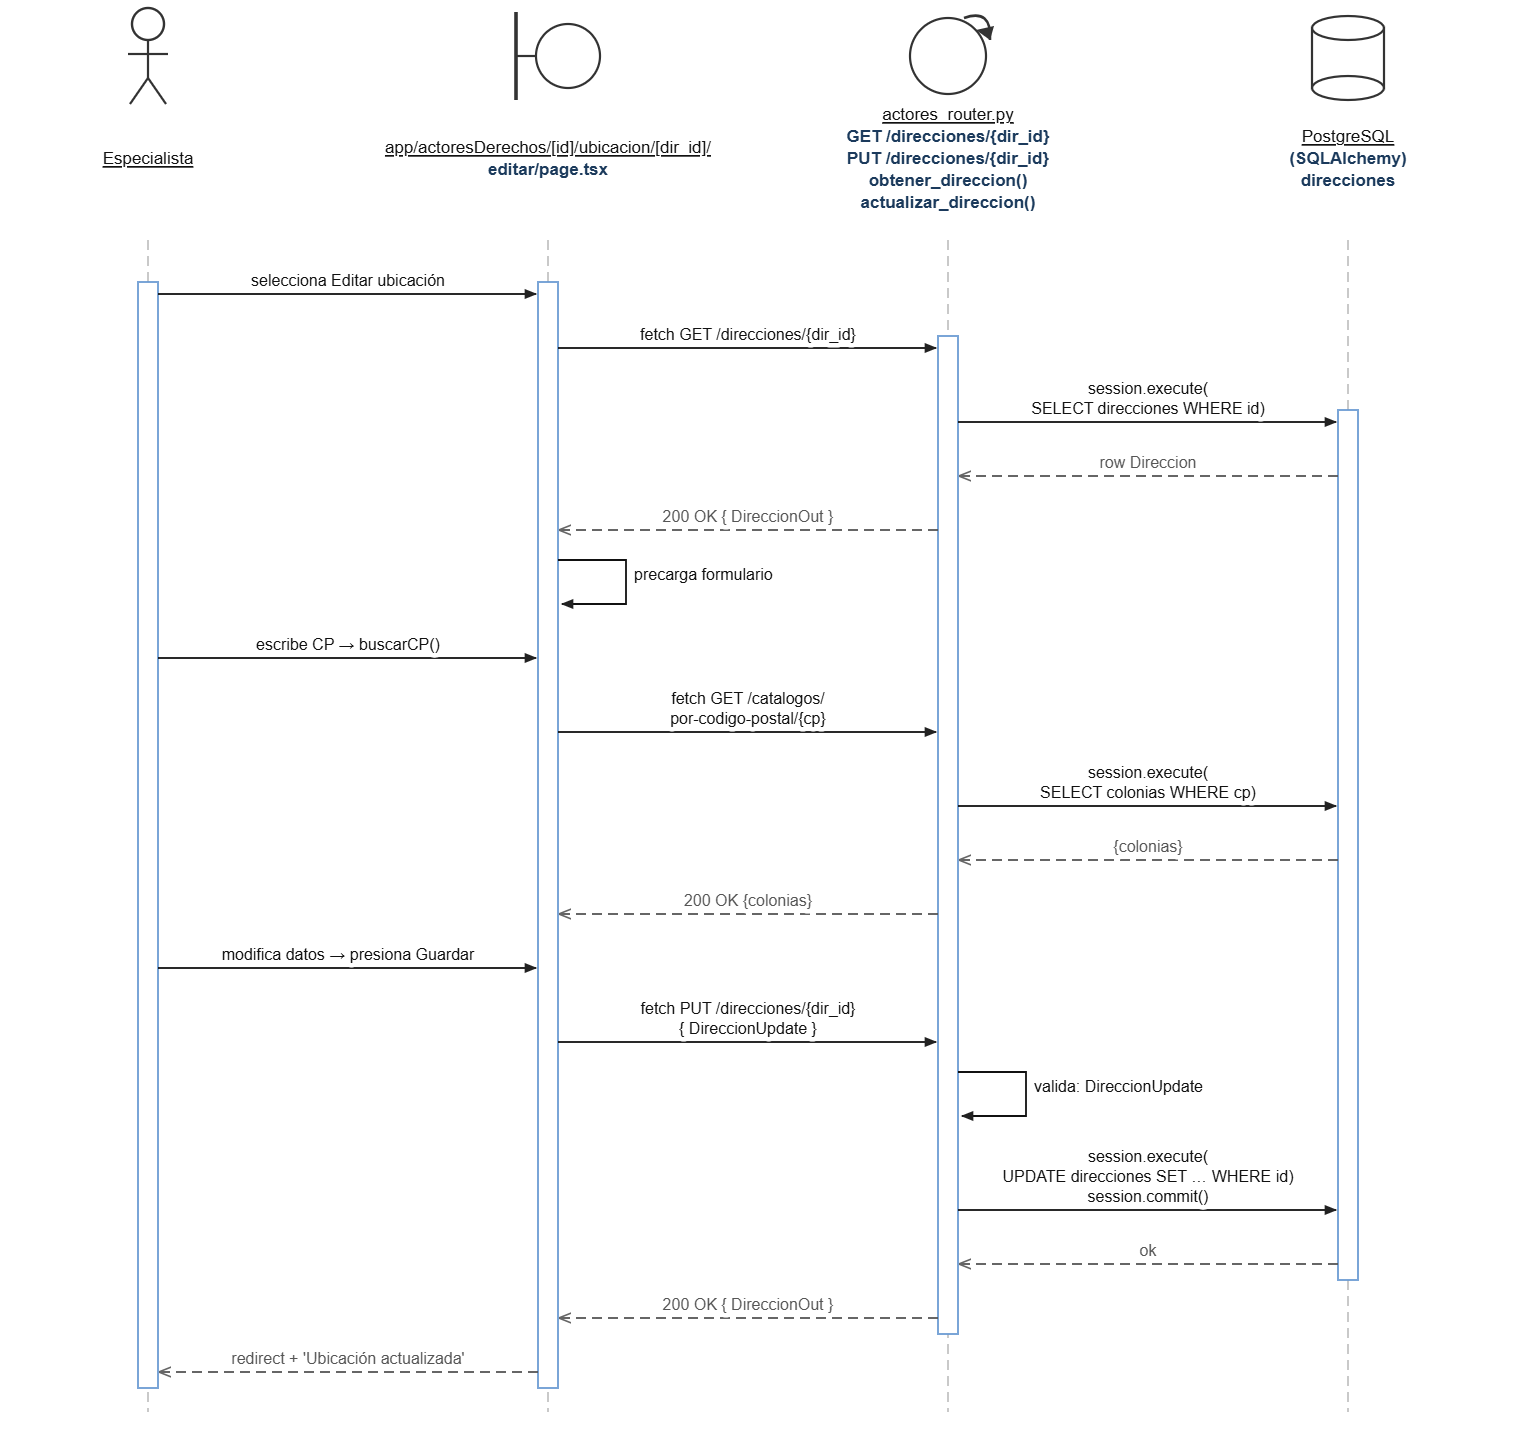
\includegraphics[width=0.8\textwidth]{img/CU-51.png}
	\caption{Diagrama de secuencia --- CU-51 Editar ubicación del actor.}
	\label{fig:secuencia-cu51}
\end{figure}

\subsection*{Flujo Alternativo / Excepciones}
\begin{itemize}
	\item \textbf{E1: Colonia o calle no especificada} - Se omiten datos obligatorios en el formulario de dirección. El sistema cancela el guardado.
\end{itemize}

\bigskip
\noindent\rule{\linewidth}{0.5pt}
\bigskip

% ============================================================
\section{Diseño Dinámico del CU: Editar programas del actor (CU-52)}
% ============================================================

\subsection*{Descripción del Flujo}
El Especialista accede a la sección de programas del actor y selecciona "Editar Programa". Modifica los datos del programa o sus servicios (requisitos, costo, etc.) y presiona "Guardar". El Backend valida la completitud de la información y actualiza los registros de programas y servicios asociados en la base de datos. El Backend responde éxito y la interfaz actualiza la lista de programas del actor.

\begin{figure}[H]
	\centering
	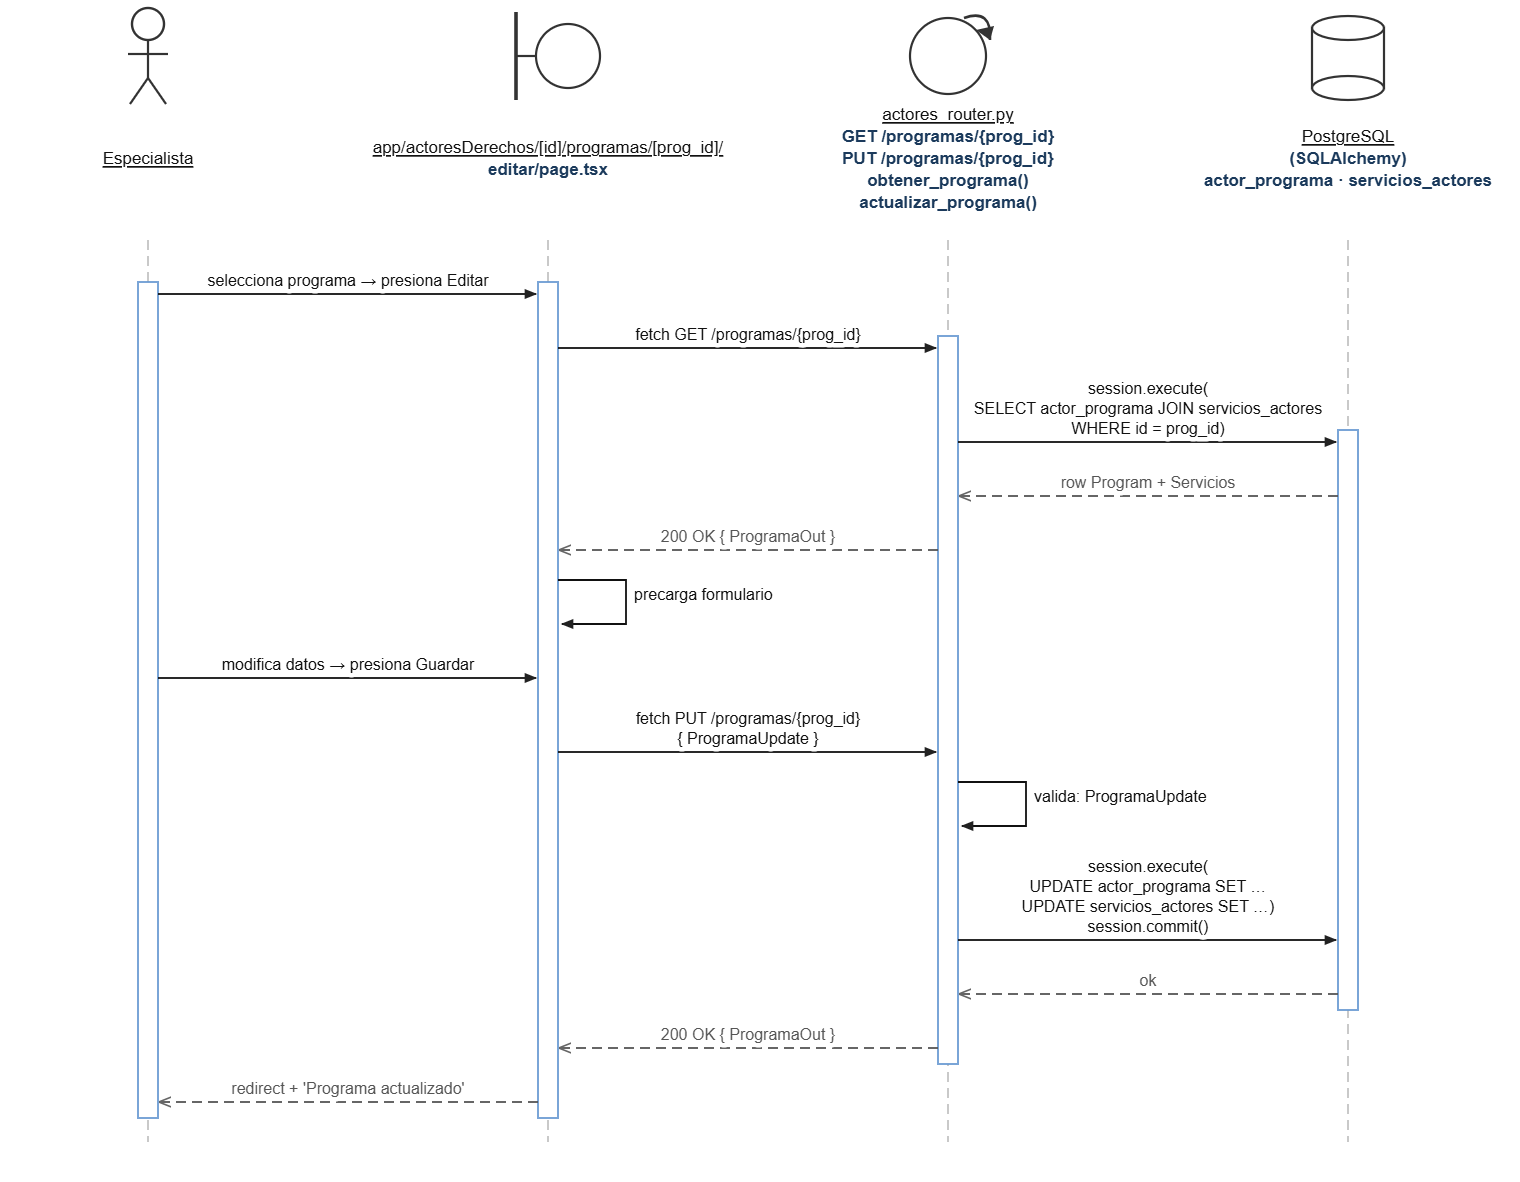
\includegraphics[width=0.8\textwidth]{img/CU-52.png}
	\caption{Diagrama de secuencia --- CU-52 Editar programas del actor.}
	\label{fig:secuencia-cu52}
\end{figure}

\subsection*{Flujo Alternativo / Excepciones}
\begin{itemize}
	\item \textbf{E1: Nombre del programa o servicio vacío} - Se borra el nombre del programa. El sistema bloquea el guardado.
	\item \textbf{E2: Formato de costo inválido} - Se ingresa un valor negativo o no numérico en el costo del servicio. El sistema cancela la edición.
\end{itemize}

\bigskip
\noindent\rule{\linewidth}{0.5pt}
\bigskip

% ============================================================
\section{Diseño Dinámico del CU: Editar enlaces representantes (CU-53)}
% ============================================================

\subsection*{Descripción del Flujo}
El Especialista edita la información de un representante de enlace de la institución aliada. Modifica su cargo, teléfono o correo y presiona "Guardar". El Backend valida que los formatos de contacto sean correctos y guarda los cambios en la tabla de representantes en la base de datos, devolviendo éxito.

\begin{figure}[H]
	\centering
	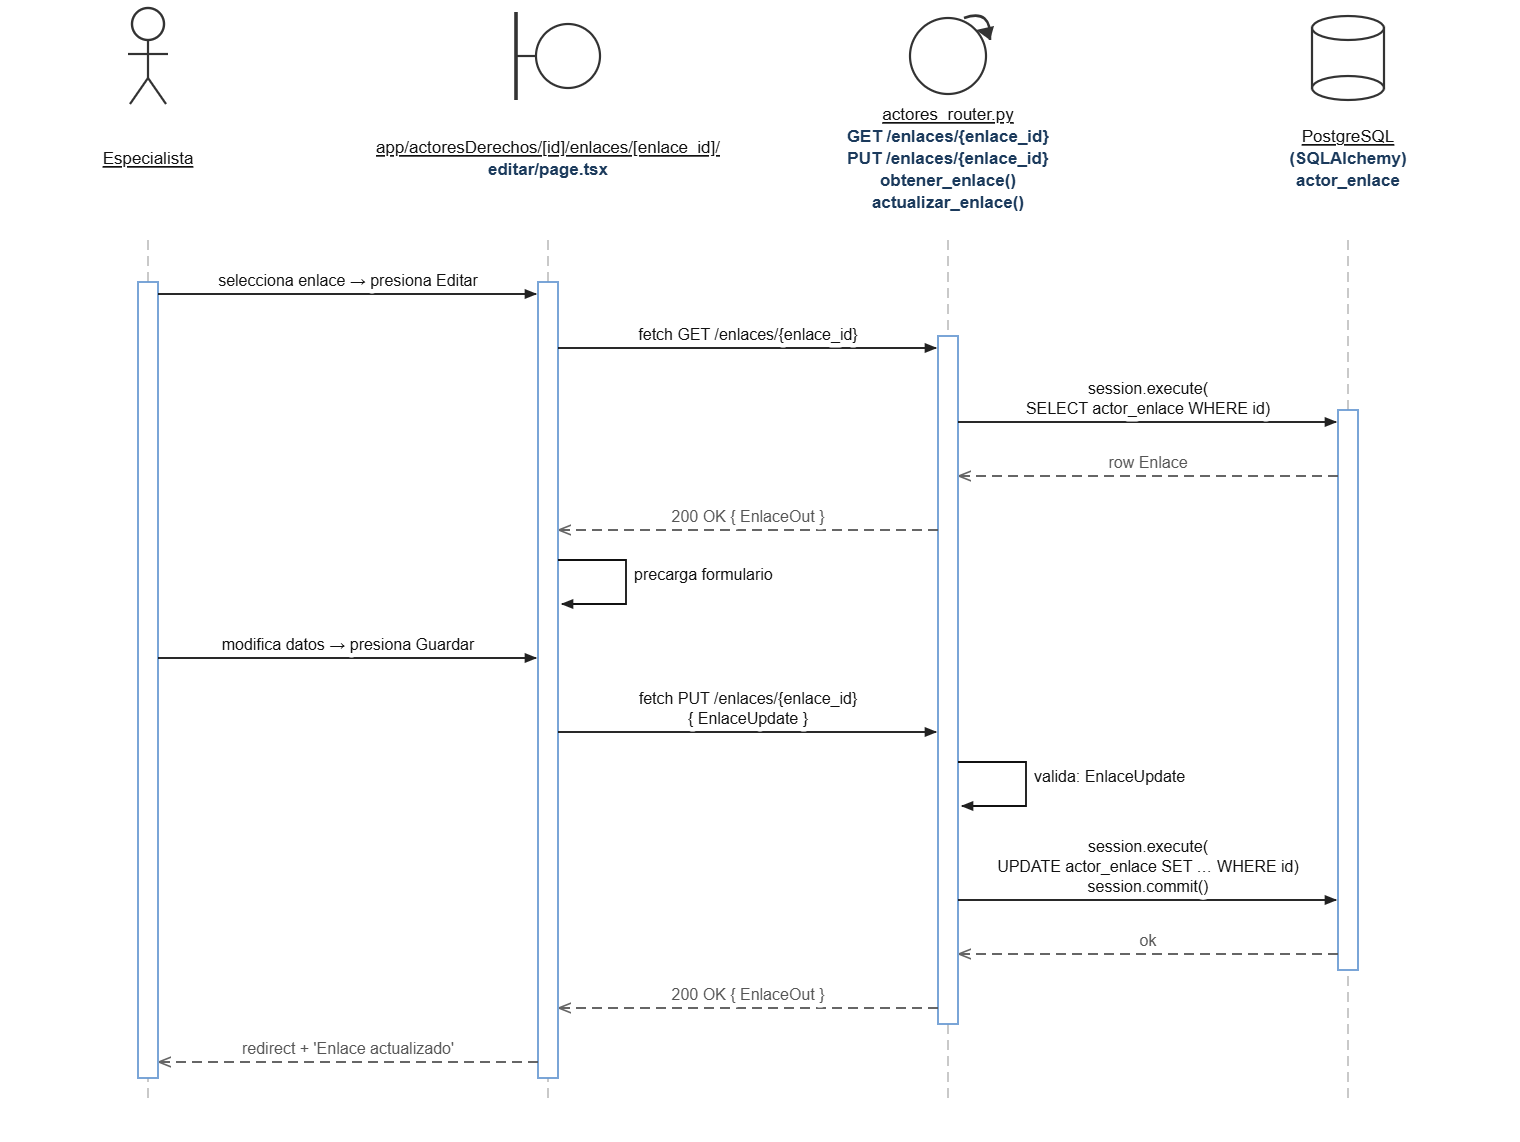
\includegraphics[width=0.8\textwidth]{img/CU-53.png}
	\caption{Diagrama de secuencia --- CU-53 Editar enlaces representantes.}
	\label{fig:secuencia-cu53}
\end{figure}

\subsection*{Flujo Alternativo / Excepciones}
\begin{itemize}
	\item \textbf{E1: Nombre del enlace en blanco} - Se intenta guardar la modificación vaciando el nombre de contacto. Se bloquea la acción.
	\item \textbf{E2: Datos de contacto con formato incorrecto} - Formatos de correo o teléfono inválidos para el representante.
\end{itemize}

\bigskip
\noindent\rule{\linewidth}{0.5pt}
\bigskip

% ============================================================
\section{Diseño Dinámico del CU: Deshabilitar actor (CU-54)}
% ============================================================

\subsection*{Descripción del Flujo}
El Especialista selecciona un actor activo del directorio y hace clic en la opción "Deshabilitar". La interfaz muestra un modal solicitando la confirmación de la inhabilitación del actor. Al confirmar, la interfaz envía la solicitud al Backend. El Backend actualiza el estado del actor a "Inactivo" en la base de datos, lo cual causa que el actor, sus programas y sus servicios dejen de figurar de forma automática en las búsquedas generales del catálogo. El Backend confirma el cambio y la interfaz actualiza el estado visual del actor en el directorio.

\begin{figure}[H]
	\centering
	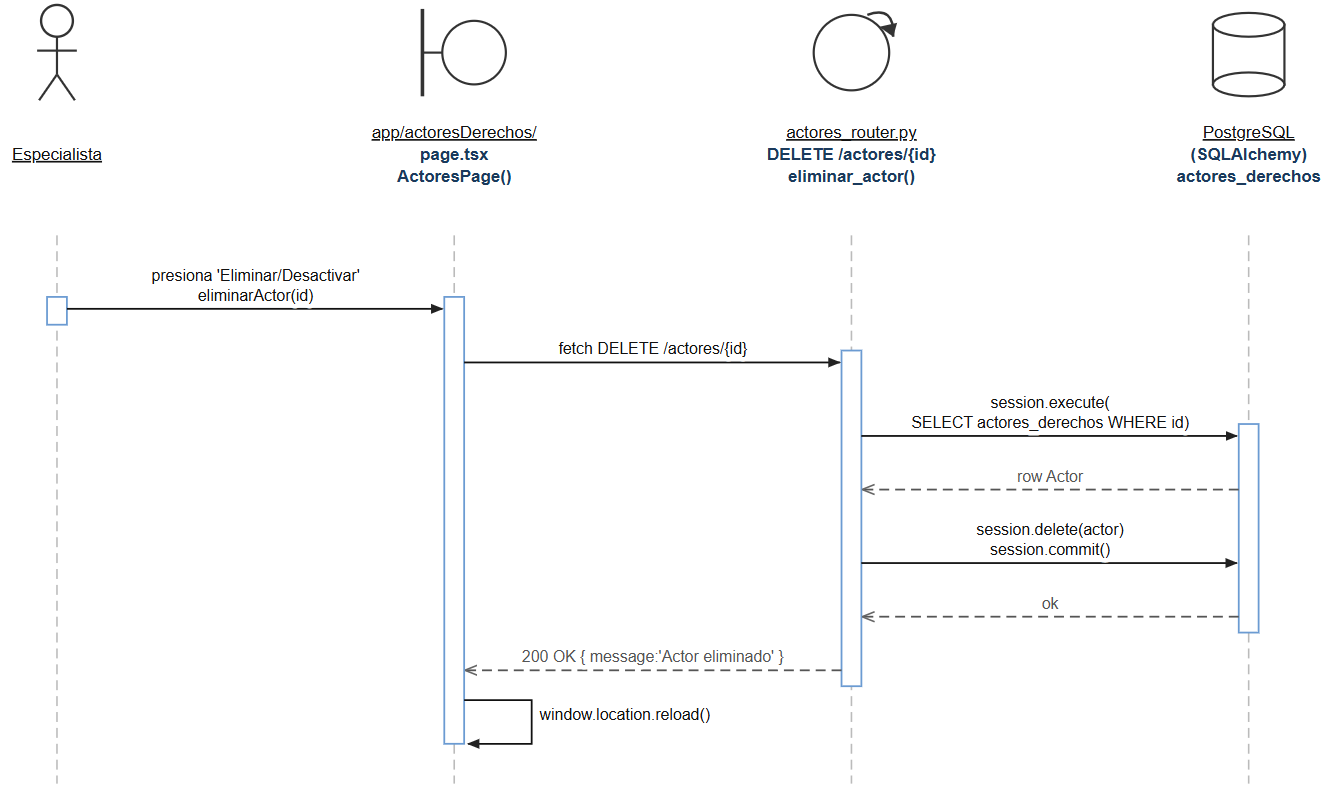
\includegraphics[width=0.8\textwidth]{img/CU54.png}
	\caption{Diagrama de secuencia --- CU-54 Deshabilitar actor.}
	\label{fig:secuencia-cu54}
\end{figure}

\subsection*{Flujo Alternativo / Excepciones}
\begin{itemize}
	\item \textbf{E1: Cancelación de la deshabilitación} - El Especialista cancela la confirmación en el modal. La interfaz cierra el modal y mantiene al actor en estado activo.
\end{itemize}

\bigskip
\noindent\rule{\linewidth}{0.5pt}
\bigskip

% ============================================================
\section{Diseño Dinámico del CU: Reactivar actor (CU-55)}
% ============================================================

\subsection*{Descripción del Flujo}
El Especialista localiza un actor con estado inactivo en el directorio y hace clic en "Reactivar". La interfaz muestra un modal solicitando la confirmación de la reactivación del actor. Al confirmar, la interfaz envía la solicitud al Backend. El Backend cambia el estado del actor a "Activo" en la base de datos, restableciendo de inmediato su visibilidad y la de sus programas asociados para nuevas búsquedas y vinculaciones. El Backend confirma la operación y la interfaz actualiza el estado visual del actor en pantalla.

\begin{figure}[H]
	\centering
	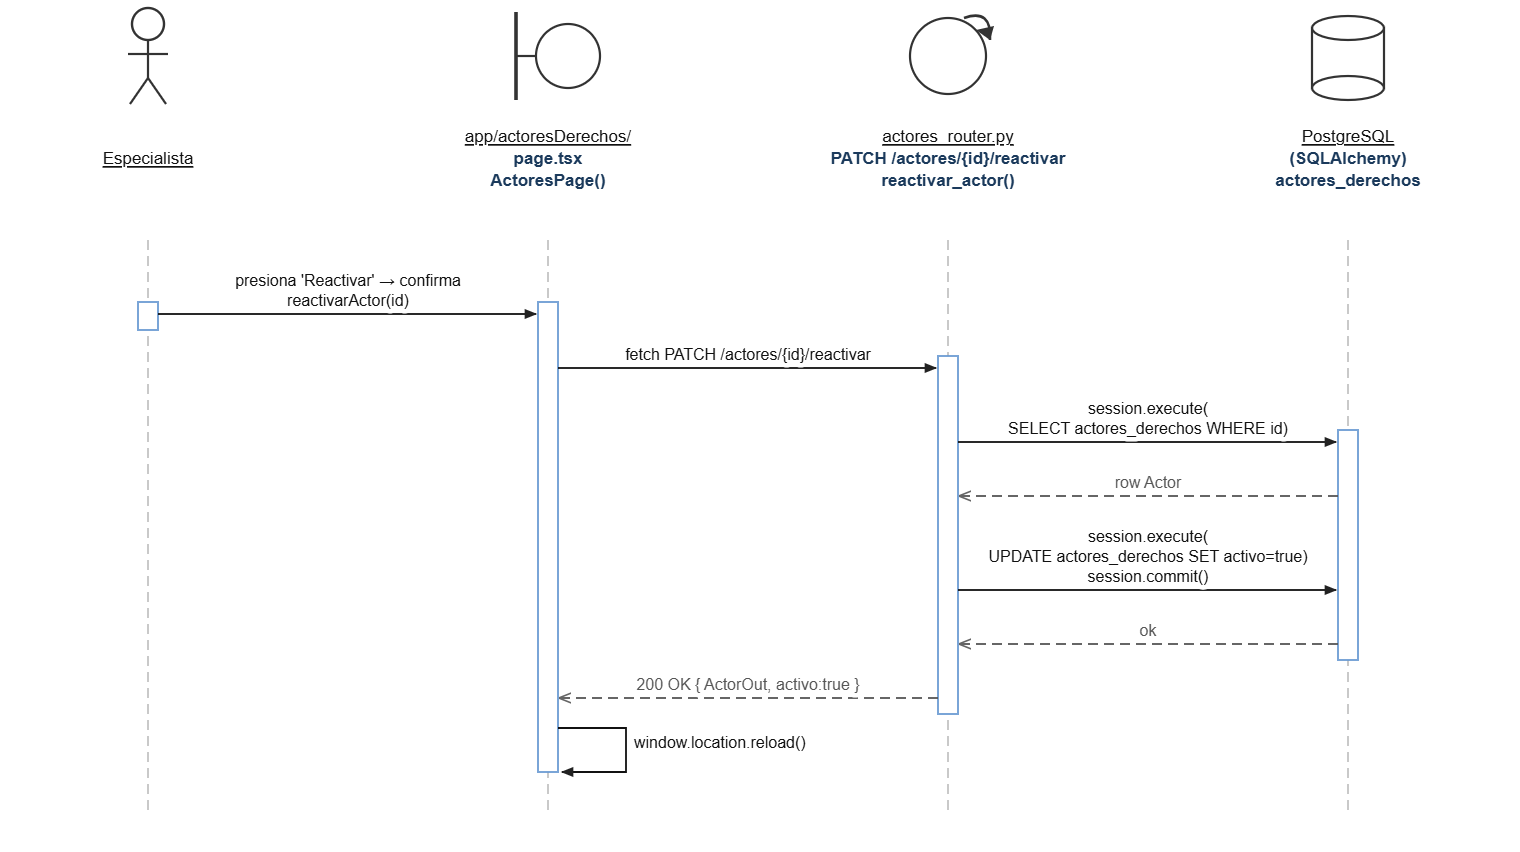
\includegraphics[width=0.8\textwidth]{img/CU-55.png}
	\caption{Diagrama de secuencia --- CU-55 Reactivar actor.}
	\label{fig:secuencia-cu55}
\end{figure}

\subsection*{Flujo Alternativo / Excepciones}
\begin{itemize}
	\item \textbf{E1: Cancelación de la reactivación} - El Especialista cancela la confirmación. La interfaz cierra el modal y mantiene al actor en estado inactivo.
\end{itemize}

\bigskip
\noindent\rule{\linewidth}{0.5pt}
\bigskip

% ============================================================
\section{Diseño Dinámico del CU: Consultar catálogo de programas (CU-56)}
% ============================================================

\subsection*{Descripción del Flujo}
El Especialista accede a la sección de consulta del catálogo de programas de apoyo. La interfaz solicita la información al Backend. El Backend ejecuta una consulta select en la base de datos sobre la tabla de programas y servicios activos, agrupándolos y vinculándolos con la información de sus respectivos actores. La base de datos devuelve los registros y el Backend los envía a la interfaz, que renderiza el catálogo en forma de una tabla o rejilla interactiva de programas.

\begin{figure}[H]
	\centering
	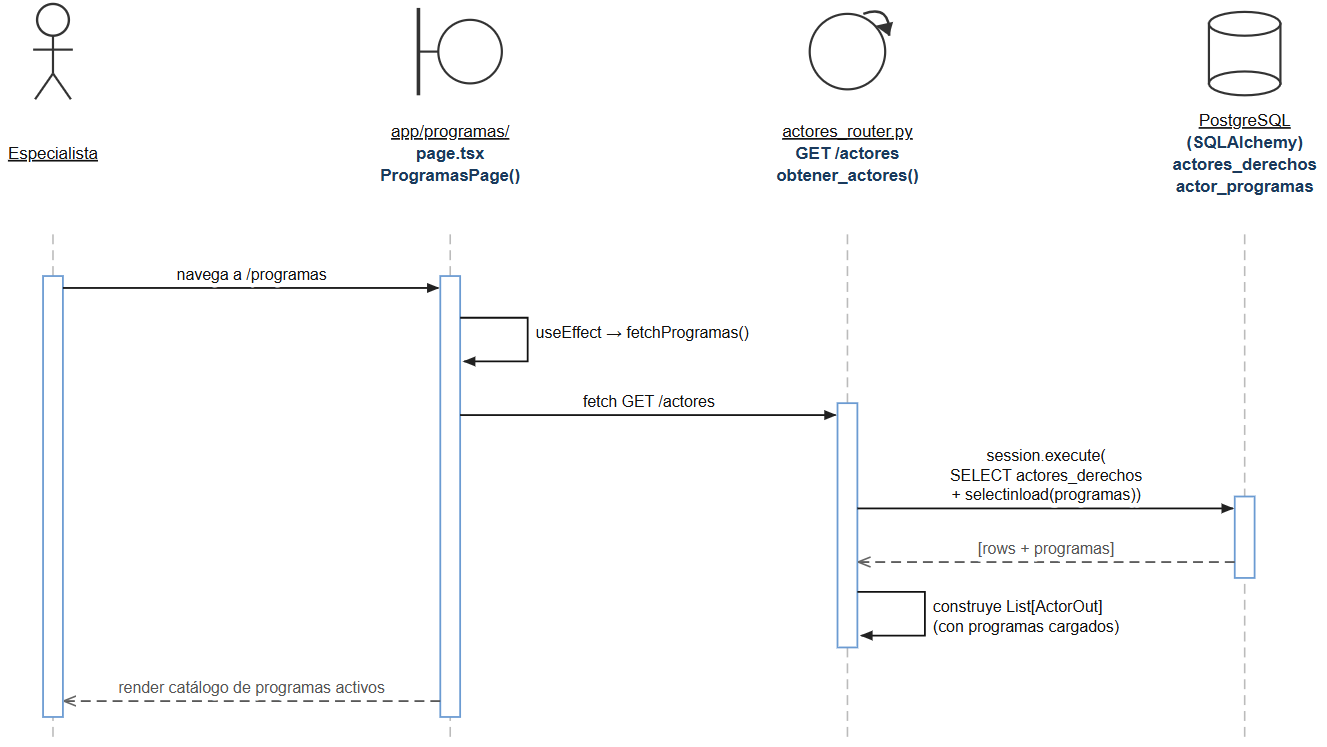
\includegraphics[width=0.8\textwidth]{img/CU56.png}
	\caption{Diagrama de secuencia --- CU-56 Consultar catálogo de programas.}
	\label{fig:secuencia-cu56}
\end{figure}

\subsection*{Flujo Alternativo / Excepciones}
\begin{itemize}
	\item \textbf{E1: No existen programas activos registrados} - Si la consulta a la base de datos está vacía, el sistema muestra una interfaz limpia junto con el mensaje "No hay programas registrados en el catálogo".
\end{itemize}

\bigskip
\noindent\rule{\linewidth}{0.5pt}
\bigskip

% ============================================================
\section{Diseño Dinámico del CU: Buscar programas (CU-57)}
% ============================================================

\subsection*{Descripción del Flujo}
El Especialista introduce un criterio de búsqueda (nombre del programa, nombre del servicio, requisitos o palabras clave) en la barra de búsqueda del catálogo de programas. La interfaz transmite el criterio al Backend. El Backend realiza una consulta select filtrada en la base de datos utilizando operadores de coincidencia de texto. La base de datos devuelve la lista de programas coincidentes y el Backend los envía a la interfaz para su despliegue en pantalla.

\begin{figure}[H]
	\centering
	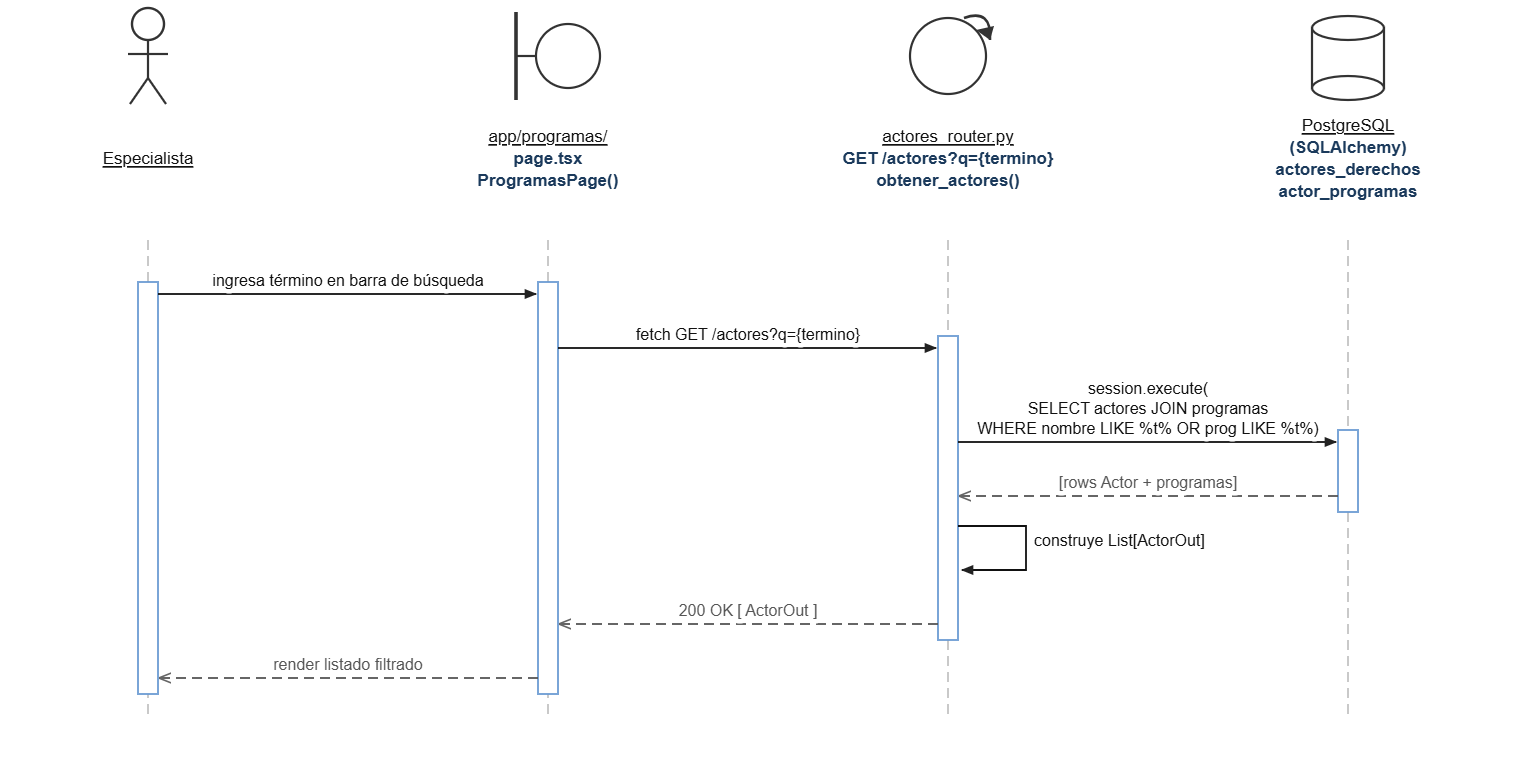
\includegraphics[width=0.8\textwidth]{img/CU-57.png}
	\caption{Diagrama de secuencia --- CU-57 Buscar programas.}
	\label{fig:secuencia-cu57}
\end{figure}

\subsection*{Flujo Alternativo / Excepciones}
\begin{itemize}
	\item \textbf{E1: Sin resultados coincidentes} - Ningún programa activo coincide con los criterios de búsqueda especificados. El sistema muestra el listado vacío con el mensaje "No se encontraron programas con el criterio ingresado".
\end{itemize}

\bigskip
\noindent\rule{\linewidth}{0.5pt}
\bigskip

% ============================================================
\section{Diseño Dinámico del CU: Deshabilitar programa (CU-58)}
% ============================================================

\subsection*{Descripción del Flujo}
El Especialista localiza un programa activo en el catálogo y hace clic en "Deshabilitar". La interfaz muestra un modal solicitando la confirmación de la inhabilitación temporal del programa. Al confirmar la acción, la interfaz envía la petición al Backend. El Backend actualiza el estado del programa a "Inactivo" en la base de datos. De este modo, sus servicios asociados dejan de estar elegibles en el catálogo general y no pueden ser vinculados a nuevos NNA. El Backend confirma el cambio y la interfaz actualiza el estado del programa en pantalla.

\begin{figure}[H]
	\centering
	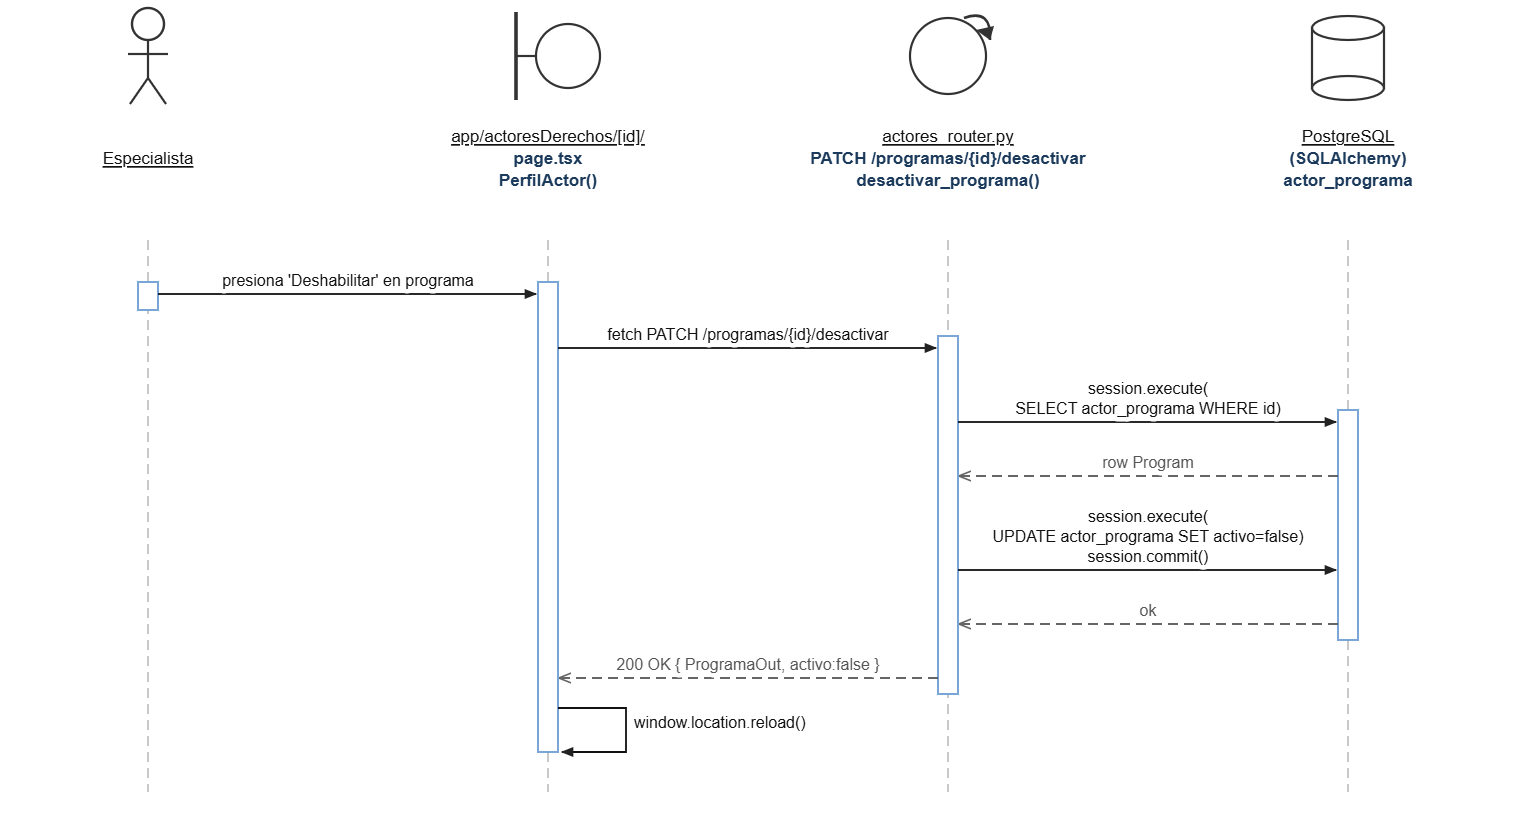
\includegraphics[width=0.8\textwidth]{img/CU-58.png}
	\caption{Diagrama de secuencia --- CU-58 Deshabilitar programa.}
	\label{fig:secuencia-cu58}
\end{figure}

\subsection*{Flujo Alternativo / Excepciones}
\begin{itemize}
	\item \textbf{E1: Cancelación de la deshabilitación} - El Especialista cancela la confirmación en el modal. La interfaz cierra el modal y mantiene el programa en estado activo.
\end{itemize}

\bigskip
\noindent\rule{\linewidth}{0.5pt}
\bigskip

% ============================================================
\section{Diseño Dinámico del CU: Reactivar programa (CU-59)}
% ============================================================

\subsection*{Descripción del Flujo}
El Especialista localiza un programa inactivo en el catálogo y hace clic en "Reactivar". La interfaz despliega un modal solicitando la confirmación. Al confirmar la reactivación, la interfaz envía la solicitud al Backend. El Backend cambia el estado del programa a "Activo" en la base de datos, de modo que sus servicios asociados vuelven a estar listados y listos para ser ofrecidos a nuevos NNA. El Backend confirma la operación y la interfaz actualiza el catálogo en pantalla.

\begin{figure}[H]
	\centering
	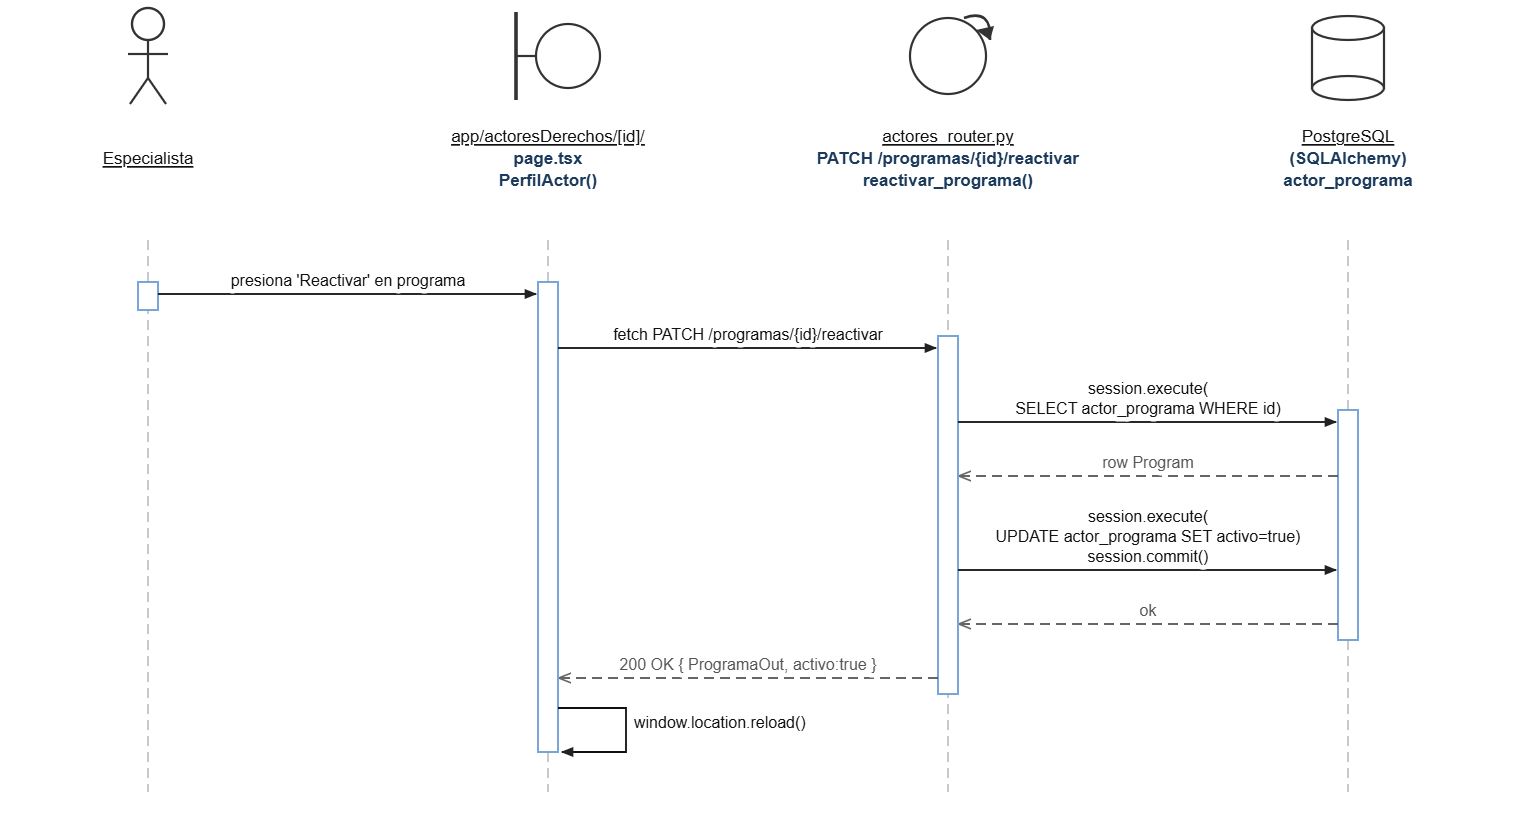
\includegraphics[width=0.8\textwidth]{img/CU-59.png}
	\caption{Diagrama de secuencia --- CU-59 Reactivar programa.}
	\label{fig:secuencia-cu59}
\end{figure}

\subsection*{Flujo Alternativo / Excepciones}
\begin{itemize}
	\item \textbf{E1: Cancelación de la reactivación} - El Especialista cancela la confirmación. El programa permanece inactivo sin cambios.
\end{itemize}
